%\documentclass[twocolumn,showpacs,nofootinbib,preprintnumbers,amsmath,amssymb]{revtex4}
\documentclass[prc,twocolumn,showpacs,preprintnumbers,amsmath,amssymb
,superscriptaddress,a4paper,nofootinbib
]{revtex4-1}

%
\usepackage{times}
\usepackage{natbib}
\usepackage{amssymb,amsbsy,amsmath,amsfonts}
\usepackage{graphicx}% Include figure files
\usepackage{epsf,epsfig,float,latexsym,amsthm,fancyhdr,rotating}
\usepackage{graphics,psfrag,longtable}
%\usepackage{srcltx}
\usepackage{slashed}
%\usepackage{footnote}
\usepackage[colorlinks,citecolor=blue,linktoc=all,linkcolor=cyan]{hyperref}

\textwidth18.5cm
\begin{document}
%\preprint{MITP/13-042}
\title {Moments of nucleon structure functions in baryon chiral perturbation theory}
\author{Jose Manuel Alarc\'on}
%\affiliation{
%Cluster of Excellence PRISMA Institut f\"ur Kernphysik, Johannes Gutenberg-Universit\"at, Mainz D-55099, Germany}
\affiliation{Helmholtz-Institut f\"ur Strahlen- und Kernphysik (Theorie) \& Bethe Center for Theoretical Physics, \\Universit\"at Bonn,
D-53115 Bonn, Germany}
\author{Franziska Hagelstein}
\affiliation{PRISMA Cluster of Excellence \& Institut f\"ur Kernphysik,
 Johannes Gutenberg-Universit\"at  Mainz,  D-55099 Mainz, Germany}
\author{Vadim Lensky}
\affiliation{PRISMA Cluster of Excellence \& Institut f\"ur Kernphysik,
 Johannes Gutenberg-Universit\"at  Mainz,  D-55099 Mainz, Germany}
\affiliation{Institute for Theoretical and Experimental Physics, Bol'shaya Cheremushkinskaya 25, 117218 Moscow, Russia}
\affiliation{National Research Nuclear University MEPhI (Moscow Engineering Physics Institute), 115409 Moscow, Russia}
\author{Vladimir Pascalutsa}
\affiliation{PRISMA Cluster of Excellence \& Institut f\"ur Kernphysik,
 Johannes Gutenberg-Universit\"at  Mainz,  D-55099 Mainz, Germany}
 \email{vladipas@kph.uni-mainz.de}

\begin{abstract}
We calculate the generalized polarizabilities and moments of the nucleon structure functions in the relativistic formulation of chiral perturbation theory with baryons. 
This calculation is a next-to-leading order prediction of the double virtual Compton scattering (VVCS) amplitude that includes the contribution of the $\Delta(1232)$ as intermediate state.
By expanding our results in powers of the inverse nucleon  mass
we reproduce the known `heavy-baryon' expressions. We
observe however that the heavy-baryon expansion of our results
converges only asymptotically. The results for the
forward spin polarizabilities $\gamma_0$ and $\delta_{LT}$
of the proton are compared with the existing expressions, while the results
for the scalar polarizabilities are new. The latter play an
important role in the calculation of nucleon structure 
effects in the muonic-hydrogen Lamb shift. 
The result for the neutron polarizability $\delta_{LT}$
is in a much better agreement with experiment than 
the corresponding heavy-baryon result, which means
the so-called ``$\delta_{LT}$ puzzle" could be explained
by relativistic effects.
\end{abstract}
%\pacs{}
\date{\today}
\maketitle

\tableofcontents

\section{Introduction}

The polarizabilities of the nucleon fully characterize its two-photon response
at low energy and hence are important for studies of nucleon structure,
most notably for the determination of the proton charge radius from
either atomic spectra or elastic electron scattering. As the ``proton
charge radius puzzle" \cite{Pohl:2010zza,Pohl:2013yb} is yet to 
see a fully satisfactory explanation, 
an accurate knowledge of nucleon polarizabilities and of the their role
in the two-photon exchange physics is ever more relevant. 

In this work we obtain the momentum-transfer ($Q^2$) behavior of
generalized nucleon polarizabilities of the doubly-virtual Compton scattering (VVCS)
process in the forward direction at next-to-leading-order (NLO) Baryon
Chiral Perturbation Theory (BChPT) including the $\Delta$ degrees of freedom.   Our results for the scalar
polarizabilities are new while the ones for the forward
spin polarizabilities $\gamma_0$ and $\delta_{LT}$ 
are compared with the recent results of
Bernard {\it et~al.}~\cite{Bernard:2012hb}. 
Upon expanding our results in powers of inverse nucleon mass, $M_N^{-1}$, we are able to reproduce the LO results
of Heavy-Baryon Chiral Perturbation Theory (HBChPT) 
which exist for the magnetic polarizability \cite{Birse:2012eb} 
and the forward spin polarizabilities~\cite{Kao:2002cp}.

In the manifestly-invariant formulation of BChPT one 

Our attitude is that the HB results can always be obtained by an expansion
of the BCHPT results in powers of inverse nucleon mass, $M_N^{-1}$, and
hence is easily available. We however do not see a rationale for
dropping the higher-order $M_N^{-1}$ terms when they are not 
negligible (i.e., when their actual size exceeds by far the natural estimate
for the size of higher-order terms).

IR, EOMS, in fact there is nothing to renormalize, let alone regularize
in the leading-order polarizability calculation as is especially evident from the validity of the sum rules.

Indeed we check that the tree-level cross sections of pion electro-production reproduce the result of the direct calculation via the VVCS amplitude.

Prediction!

The interest on the proton polarizabilities has increased since the experimental determination of the proton radius \cite{Pohl:2010zza} from muonic hydrogen has determined a value that is $7\sigma$ away from the value determined from normal hydrogen and $e\,p$ scattering \cite{Bernauer:2010wm} . This is because the $\sim 300$~$\mu$eV of disagreement in the Lamb shift measurement between muonic hydrogen ($\mu H$) and normal hydrogen ($eH$) atom could be due to the internal electromagnetic structure of the proton, since for $\mu H$ the muon is much closer to the proton and is much more influenced by its internal electromagnetic structure.

The information about the polarizabilities can be accessed through experimental information through different sum rules that involve the cross sections of the inclusive processes \cite{Drechsel:2002ar}. 
For example, for real forward Compton scattering one can connect the sum of the electric and magnetic polarizabilities of the nucleon to its total photoabsorption cross section through the Baldin sum rule \cite{BaldinSumRule}. Also, the GDH sum rule \cite{Gerasimov:1965et,Drell:1966jv} provides information about the nucleons anomalous magnetic moments in terms of the helicity difference photoabsorption cross section $\Delta\sigma=\sigma_{3/2}-\sigma_{1/2}$. This has been subject of several experiments some years ago \cite{Ahrens:2001qt, Helbing:2002eg}.
These sum rules can be generalized to the virtual photon case with virtuality $Q^2$ \cite{Drechsel:2002ar}, where the virtual photon produced in the electroproduction process acts as a probe whose resolution depends on $Q^2$, giving information about the density of polarization inside the nucleon.

In this paper, we compute the VVCS amplitude in chiral effective field theory to make parameter-free prediction of the polarizabilities of the proton and neutron at NLO. As we will show in Sec.~\ref{Sec:Scalar-Pol}, in this way we predict a high $Q^2$ behavior for the polarizabilities that makes them suitable to compute the corrections of the muonic hydrogen Lamb shift \cite{Alarcon:2013cba}. We also provide, for first time in the literature, a calculation of the longitudinal polarizability $\alpha_L(Q^2)$ from effective field theory and the $Q^2$ dependence predicted from covariant BChPT calculation for the scalar polarizabilities.

This paper is organized as follows: In Sec~\ref{Sec:Formalism} we develop the formalism we used to make our calculations, in Secs.~\ref{Sec:Scalar-Pol}-\ref{Sec:GeneralizedGDH} we show the results concerning the proton and neutron polarizabilities and some interesting moments of their structure functions. Finally,  Sec.~\ref{Sec:Summary} we summarize the results obtained here remarking the improvements done respect to previous calculations and future applications. We also include some appendices where we analyze some technical details involved in the calculation and show the analytical results of the $\pi N$ contribution to the polarizabilities and their slopes at the real photon point in a covariant form. 



\section{Formalism} 
\label{Sec:Formalism}

The forward VVCS amplitude can be parametrized by four 
scalar functions,
\begin{widetext}
\begin{align}\label{Eq:T-Compt-definition}
T(\nu,Q^2)=f_{L}(\nu,Q^2) +(\vec{\epsilon}^{\, \prime *} \cdot \vec{\epsilon}) f_{T}(\nu,Q^2)  +  i \vec{\sigma}\cdot (\vec{\epsilon}^{\, \prime *} \times \vec{\epsilon}) g_{TT}(\nu,Q^2) -  i \vec{\sigma}\cdot [(\vec{\epsilon}^{\, \prime *} - \vec{\epsilon})\times \hat{q}] g_{LT}(\nu,Q^2) 
\end{align}
\end{widetext}

where $Q^2=-q^2$ is the virtuality of the photon and $\nu=(s-M_N^2+Q^2)/2M_N$ is the energy of the photon in the lab system.
This energy variable $\nu$ is frequently used for application of dispersive methods because is odd under crossing, $\nu \to -\nu$.

Regarding the functions $f_i$ and $g_i$, two of them are independent of the spin ($f_T$ and $f_L$) while the other two ($g_{TT}$ and $g_{LT}$) are spin-dependent. 
In the real photon case, $Q^2=0$, the functions that involve longitudinal polarization ($f_L$ and $g_{LT}$) cancel, and only $f_T$ and $g_{TT}$ survive. 
Low, and Gell-Mann and Goldberger \cite{LET} proved in the 50's that the leading terms of the low energy expansions are determined uniquely by the global properties of the system, as the charge, mass and the anomalous magnetic moment. 
The polarizabilities enter as a higher order corrections and are related to the internal structure of the nucleon. 
This can be accessed through photoabsorption experiments (see Sec.~\ref{Sec:ConnectionWithElectroproduction}).

Constructed from Lorentz and gauge invariance, and crossing symmetry, one can deduce the general structures 

\begin{align}
 & f_T(\nu, Q^2)= f_T^{(B)}(\nu, Q^2) + 4 \pi Q^2 \beta_{M1} + 4 \pi(\alpha_{E1} + \beta_{M1}) \nu^2 + \dots \label{Eq:LEX-fT}\\
 & f_L(\nu, Q^2)= f_L^{(B)}(\nu, Q^2) + 4 \pi(\alpha_{E1}+\alpha_{L} \nu^2) Q^2 + \dots \label{Eq:LEX-fL}\\
 & g_{TT}(\nu, Q^2)=g^{(B)}_{TT}(\nu, Q^2) + 4 \pi\gamma_0  \nu^3 + \dots \label{Eq:LEX-gTT}\\
 & g_{LT}(\nu, Q^2)=g^{(B)}_{LT}(\nu, Q^2) +  4 \pi\delta_{LT} \nu^2 Q + \dots \label{Eq:LEX-gLT}
\end{align}

where the Born terms are \cite{Drechsel:2002ar}

\begin{align}
 & f_T^{(B)}(\nu, Q^2) =  - \frac{4\pi \alpha_{em}}{M_N} \Big( F_D^2 + \frac{\nu_B^2 G_M^2}{\nu^2-\nu_B^2} \Big) \label{Eq:BT-fT}\\
  &  f_L^{(B)}(\nu, Q^2) = - \frac{\pi \alpha_{em} Q^2}{ M_N^3} \Big( F_P^2 + \frac{4M_N^2 G_E^2}{\nu^2-\nu_B^2} \Big) \label{Eq:BT-fL}\\
 & g^{(B)}_{TT}(\nu, Q^2) = - \frac{2\pi \alpha_{em} \nu}{ M_N^2} \Big( F_P^2 + \frac{Q^2 G_M^2}{\nu^2-\nu_B^2} \Big) \label{Eq:BT-gTT}\\
 & g^{(B)}_{LT}(\nu, Q^2) =  \frac{2 \pi\alpha_{em} Q}{M_N^2} \Big( F_D F_P - \frac{Q^2 G_E G_M }{\nu^2-\nu_B^2} \Big) \label{Eq:BT-gTL}
\end{align}

with $\alpha_{em}$ the fine structure constant, $\nu_B=Q^2/2M_N$, $G_E(Q^2)$ and $G_M(Q^2)$ the electric and magnetic Sachs form factors, which are related to the Dirac ($F_D(Q^2)$) and Pauli ($F_P(Q^2)$) form factors in the following way

\begin{align}
& G_E(Q^2)=F_D(Q^2) - \frac{Q^2}{4M_N^2} F_P(Q^2)\\
& G_M(Q^2)=F_D(Q^2) + F_P(Q^2).
\end{align}



The $Q^2$ dependent functions $\alpha_{E1}$, $\beta_{M1}$, $\alpha_{L}$, $\gamma_{0}$ and $\delta_{LT}$ are the so-called generalized polarizabilities (GP), which generalize the response of the nucleon to the case of finite momentum transfer. Notice that $\alpha_L$ is usually defined including the $Q^2$ proportionality that stems from gauge invariance. 
In this case, we think it is more natural to take the $Q^2$ term out of the definition, as is usually done with $Q$ in $\delta_{LT}$.

In a covariant approach, as the one we follow in this work, the Compton tensor in the forward limit has the following tensor decomposition

\begin{widetext}
\begin{align}\label{Eq:T-Rel}
T(\nu,Q^2) = \epsilon_{\mu}^{\prime *} \epsilon_\nu \Big\{  \Big( -g^{\mu \nu} + \frac{q^\mu q^\nu}{q^2} \Big) T_1(\nu,Q^2) + \frac{1}{M_N^2} \Big(  p^\mu - \frac{p\cdot q}{q^2} q^\mu \Big) \Big(  p^\nu - \frac{p\cdot q}{q^2} q^\nu \Big) T_2(\nu,Q^2) \nonumber \\ 
                  +  \frac{i}{M_N} \epsilon^{\mu \nu \alpha \beta} q_\alpha s_\beta S_1(\nu,Q^2)   +\frac{i}{M_N^3} \epsilon^{\mu \nu \alpha \beta} q_\alpha (p\cdot q  s_\beta -s\cdot q  p_\beta ) S_2(\nu,Q^2)      \Big\} 
\end{align}
\end{widetext}
where $s^\mu$ is the covariant spin tensor which satisfy $s\cdot p=0$ and $s^2=-1$, and the normalization of the Levi-Civita tensor is $\epsilon_{0123}=+1$. 

In order to extract the GP it will be useful to keep in mind the relation between the relativistic \eqref{Eq:T-Rel} and non-relativistic forms \eqref{Eq:T-Compt-definition}
\begin{align}
 & f_T(\nu,Q^2) = T_1(\nu,Q^2) \label{Eq:fT-T1}\\
 & f_L(\nu,Q^2) = - T_1(\nu,Q^2) +  \frac{\nu^2 + Q^2}{Q^2} T_2(\nu,Q^2) \label{Eq:fL-T1T2}\\
 & g_{TT}(\nu, Q^2) = \frac{\nu}{M_N}\Big( S_1(\nu,Q^2) - \frac{Q^2}{M_N\,\nu} S_2(\nu,Q^2)\Big)\label{Eq:gTT-S1S2}\\
 & g_{LT}(\nu, Q^2) = \frac{Q}{M_N}\Big( S_1(\nu,Q^2) + \frac{\nu}{M_N} S_2(\nu,Q^2)\Big)\label{Eq:gLT-S1S2}
\end{align} 
therefore, the polarizabilities can be obtained from linear combinations of the Born-subtracted functions $T_1$, $T_2$, $S_1$, $S_2$. 

% {\bf (Vadim: Here we could write all the details of the VVCS calculation in ChPT)}

We calculate these amplitudes in the relativistic formulation of chiral effective field theory with baryons
including the $\Delta(1232)$-resonance as a dynamical degree of freedom.
This calculation generalizes the work of ref.~\cite{Lensky:2009uv} to the case of virtual photons in the forward kinematics.
The potential of the covariant formalism once the $\Delta(1232)$ is included as an explicit degree of freedom
has been also observed in other chiral analyses, e.g., of $\pi N$ scattering~\cite{Alarcon:2012kn,Chen:2012nx}
and $\pi N \to \pi \pi N$ \cite{Siemens:2014pma}. Note that the chiral approaches at NLO in the $\delta$-counting
provide predictions of the polarisabilities, since up to that order they are free of low-energy constants.

We employ the chiral Lagrangian for the pion and nucleon fields, see e.g.~\cite{GSS89}. Up to the second order in the pion field, it takes the form
\begin{widetext}
\begin{align}
\mathcal{L}^{(1)}_{N}  =  \overline{N}\left( i \slashed{\partial} -{M}_{N}
+ \frac{g_A}{2f_\pi} \tau^a \slashed{\partial}\,\pi^a\gamma_5 - \frac{1}{4f_\pi^2} \, \tau^a \epsilon^{abc}  \pi^b\,\slashed{\partial} \,\pi^c
\right) N  + \mathcal{O}(\pi^3) \,,
\label{expNlagran}
\end{align}
\end{widetext}
% As shown, Ref~\cite{Lensky:2009uv},  after a chiral rotation of the nucleon field the Lagrangian takes the form
% 
% \begin{align}
% {\mathcal{L}'}_{\pi N}^{(1)} =   \overline{N}\left( i \slashed{\partial} -{m}_{N}
% - 
% i\, \frac{ g_A}{f_\pi} M_N \tau^a\pi^a\gamma_5 +  \frac{g_A^2}{2f_\pi^2} M_N \pi^2
%  +\frac{(g_A^2-1)}{4f_\pi^2} \, \tau^a\epsilon^{abc}  \pi^b\,\slashed{\partial} \,\pi^c
% \right) N
%  + \mathcal{O}(\pi^3)\,,\nonumber\\
% \label{expNlagran2}
% \end{align}
% 
% where $N(x)$ and $M_N$ is the nucleon field and mass respectively, $\pi^a(x)$ is the pion field, the $\tau^a$ are the Pauli matrices and $\epsilon^{abc}$ is the Levi-Civita tensor; $g_A\simeq 1.27$, $f_\pi\simeq 92.4$~MeV. 
% Upon the minimal inclusion of the electromagnetic field, the two Lagrangians give identical results for the $O(p^3)$ Compton scattering amplitude and the isovector term proportional to $(g_A^2-1)$ does not contribute. 
% Working with the rotated Lagrangian, however, simplifies considerably the calculation. 
The Lagrangians of the $\Delta(1232)$ and its coupling to the nucleons and pions are~\cite{Pascalutsa:2002pi,Lensky:2009uv}:
\begin{eqnarray}
\mathcal{L}^{(1)}_{\Delta} &=& \overline\Delta_\mu \left(i\gamma^{\mu\nu\lambda}\,\partial_\lambda - 
M_\Delta\,\gamma^{\mu\nu}\right) \Delta_\nu \nonumber\\
&+&  \frac{i\,h_A}{2f_\pi M_\Delta}
\left[
i \overline N\, T_a%^\dagger
 \,\gamma^{\mu\nu\lambda}\, (\partial_\mu \Delta_\nu)\, \partial_\lambda\pi^a
+ \mbox{H.c.}\right],
\end{eqnarray}
The electromagnetic interaction is added via the minimal substitution:
\begin{subequations}
\begin{eqnarray}
\partial_\mu N &\to & \partial_\mu N -  i e A_\mu\frac{1}{2}(1+\tau_3) N ,\\
\partial_\mu \pi^a &\to & \partial_\mu \pi^a - eA_\mu\epsilon^{ab3}\pi^b\,,
\end{eqnarray}
\end{subequations}
where $A_\mu$ is the photon field. The minimal coupling of the photon to the Delta field gives contributions to Compton scattering which are of higher orders than the ones considered in this work.

% Apart from these Lagrangians, there are the following nonminimal terms:
% \begin{subequations}
% \begin{eqnarray}
% \mathcal{L}^{(2)}_N &=&  \frac{e\kappa_{p,n}}{4M_N} 
% \,\overline N\,\frac{1}{2} (1\pm \tau_3) \,\gamma^{\mu\nu}\, N \,F_{\mu\nu} , \\
% \mathcal{L}^{(2)}_\Delta &=&  \frac{3e}{2M_N(M_N+M_\Delta)}\,\overline N\, T_3
% \left(i g_M  \tilde F^{\mu\nu} - g_E \gamma_5 F^{\mu\nu}\right)\,\partial_{\mu}\Delta_\nu
% + \mbox{H.c.},
% \\
% \mathcal{L}^{(4)}_{\mathrm{WZW}}&=&  -\frac{e^2 }{32\pi^2 f} F_{\mu\nu} \tilde F^{\mu\nu}\pi_3 \, .\nonumber
% \end{eqnarray}
% \end{subequations}
% Here, $F^{\mu\nu}$ and $\tilde F^{\mu\nu}$ are the photon field strength tensor and its dual tensor defined
% as $F^{\mu\nu}=\partial^\mu A^\nu-\partial^\nu A^\mu$, $\tilde F^{\mu\nu}=\frac{1}{2}\epsilon^{\mu\nu\rho\lambda}F_{\rho\lambda}$;
% $\kappa_p$ ($\kappa_n$) stands for the proton's (neutron's) anomalous magnetic moment; 
% $g_E$ and $g_M$ are $\gamma N\Delta$ electric and magnetic couplings, respectively,
% which are known from the analysis of pion-photoproduction $P_{33}$ multipoles~\cite{Pascalutsa:2005ts}. Of these nonminimal Lagrangians,
% only $\mathcal{L}^{(2)}_\Delta$ contributes to the polarisabilities.

Apart from these Lagrangians, there is the following non-minimal $\gamma N\Delta$ coupling~\cite{Pascalutsa:2005ts} that contributes
to the polarizabilities: \footnote{Note that here we corrected a typo appearing in \cite{Pascalutsa:2005ts,Pascalutsa:2005vq,Pascalutsa:2006up}.}
\begin{eqnarray}
\mathcal{L}^{(2)}_\Delta &=&  \frac{3e}{2M_N(M_N+M_\Delta)}\,\overline N\, T_3\left\{
\left(i g_M  \tilde F^{\mu\nu} - g_E \gamma_5 F^{\mu\nu}\right)\,\partial_{\mu}\Delta_\nu\right. \nonumber\\
&+&\left.i \frac{g_C}{M_\Delta}\gamma_5 \gamma^\alpha (\partial_\alpha \Delta_\nu-\partial_\nu \Delta_\alpha)\partial_\mu F^{\mu \nu} \right\}+\mbox{H.c.}.
\end{eqnarray}
Here, $F^{\mu\nu}$ and $\tilde F^{\mu\nu}$ are the photon field strength tensor and its dual tensor defined
as $F^{\mu\nu}=\partial^\mu A^\nu-\partial^\nu A^\mu$, $\tilde F^{\mu\nu}=\frac{1}{2}\epsilon^{\mu\nu\rho\lambda}F_{\rho\lambda}$,
and  $g_E$ and $g_M$ are $\gamma N\Delta$ electric and magnetic couplings, respectively,
which are known from the analysis of pion-photoproduction $P_{33}$ multipoles~\cite{Pascalutsa:2005ts}.

The values of the above defined physical constants used in this work are given in Table~\ref{tab:constants}.

\begin{table}[hbt]
\begin{tabular}{|c|c||c|c|}
\hline
$\alpha_{\rm EM}$ & $1/(137.04)$&
$f_\pi$ & $92.21$ MeV \\
$m_\pi^{\pm}$ & $139.57$ MeV &
%$m_\pi^0$ & 134.98 MeV\\
$M_N=M_p$ & $938.27$ MeV\\
$g_A$ & 1.270 &
%$\kappa^{\rm (s)}$ & $-0.120$\\ 
%$\kappa^{\rm (v)}$ & $3.706$ \\
%$\kappa^{\rm (p)}$ & $1.793$ \\
&  \\
$M_\Delta$ & $1232$ MeV&
$h_A\equiv 2g_{\pi N \Delta}$& $2.85$\\
$g_M$ & $2.97$ & $g_E$ & $-1.0$\\
\hline
\end{tabular}
\caption{Common parameters used in our calculation, see ref.~\cite{Agashe:2014kda}.
The $\pi$N$\Delta$ coupling constant $h_A$ is fit to the the experimental Delta width and the magnetic and electric $\gamma$N$\Delta$ coupling constants $g_M$ and $g_E$
are taken from the pion photoproduction study of Ref.~\cite{Pascalutsa:2005vq}}
\label{tab:constants}
\end{table}
The Feynman diagrams that one has to evaluate are shown in Figs.~\ref{Fig:loops_pv} and \ref{Fig:loopsD}
\footnote{Note that a chiral rotation of the nucleon field can considerably simplify the calculation of the $\pi N$ one-loop diagrams~\cite{Lensky:2009uv}.}.
 In analogy with Ref.~\cite{Pascalutsa:2005vq} we take into account the effect of the $\gamma^* N \Delta$ transition form factor
(entering the corresponding vertex in the Delta pole graph in Fig.~\ref{Fig:loopsD}) by introducing the following running
of the magnetic $\gamma N\Delta$ coupling:
\begin{align}
g_M \to \frac{g_M}{(1+ Q^2/\Lambda^2 )^2 }
\end{align} 
where $\Lambda=\sqrt{0.71~\text{GeV}^2}\approx 0.84$~GeV. 
The inclusion of this $Q^2$ dependence is motivated by previous works that point out the important of this form factor in the correct reproduction of the electroproduction data \cite{Pascalutsa:2005vq}. 
As we mention in Sec.~\ref{Sec:ConnectionWithElectroproduction}, electroproduction is directly connected with the polarizabilities and moments of the structure functions via sum rules. 
 So it is understandable that a better description of the electroproduction data will lead to a better description of the $Q^2$ behaviour of the polarizabilities and moments.
  For every quantity in which this coupling appears, we will study the effect of the dipole form introduced. 
 
 


Our approach to evaluation of the loop diagrams in Figs.~\ref{Fig:loops_pv} and \ref{Fig:loopsD} closely follows that of ref.~\cite{Lensky:2009uv},
with the necessary modifications due to the different kinematical regime. In particular, the gauge condition used in refs.~\cite{Pascalutsa:2002pi,Lensky:2009uv}
is dropped, and the terms relevant for the virtual photon case are restored everywhere in the loop integrals.
The latter are first written in the Feynman parameterisation, and the covariant amplitudes $T_{1,2}(\nu,Q^2)$, $S_{1,2}(\nu,Q^2)$
are obtained by matching the corresponding tensor structures, see Eq.(\ref{Eq:T-Rel}).
It is interesting to note that the tensor decomposition provides a non-trivial test of the calculation: we encountered additional tensor structures
that violated the gauge invariance; however, the scalar integrals over the Feynman parameters that multiplied these non-gauge-invariant structures
vanished after evaluation.

As said above, $\pi \Delta$ loop graphs where photons couple minimally to Delta contain more 
than one Delta propagator and therefore should be suppressed by extra powers of $p/\varDelta$.
However, their lower-order contributions are important for electromagnetic gauge-invariance and therefore for the 
renormalization program. In particular, the lower-order contributions of chiral loops should not affect the result of the low-energy
theorem (LET)~\cite{Low:1954kd}, and this condition is automatically satisfied for a subclass of graphs which obeys gauge invariance. The loop graphs in 
Fig.~\ref{Fig:loopsD} form such a subclass for the case of neutral Delta. In reality the Delta comes in four charge states (isospin $3/2$), and hence a 
gauge-invariant set will in addition have the higher-order graphs where photon couples minimally to the $\Delta$. To make the subclass of loop graphs 
in Fig.~\ref{Fig:loopsD} gauge invariant without the higher-order graphs, we used the same procedure as in ref.~\cite{Lensky:2009uv},
whereby the one-particle-irreducible (1PI) graphs in~\ref{Fig:loopsD} are computed with the correct isospin factors, i.e., summing over all charge 
states of the $\Delta$, whereas the isospin factors for the one-particle reducible (1PR) graphs are chosen such that their ratio to the isospin factors
of 1PI graphs is the same as in the neutral Delta case. This procedure automatically ensures exact gauge invariance and thus 
effectively includes the lower-order contributions of the one-loop graphs with minimal coupling of photons to the Delta. In case when the latter graphs 
are included explicitly, the isospin factors of 1PR graphs can be restored to actual values.
The corresponding change in the values of the polarizabilities, however, is of higher order than we consider in this work.

The renormalization proceeds in the same way as described in ref.~\cite{Lensky:2009uv}, with an important modification: as argued in
ref.~\cite{Birse:2012eb} (see also~\cite{Alarcon:2013cba}), we subtract from the $\gamma NN$ loop graphs that enter the 1PR graphs
the structures that correspond to the on-shell elastic nucleon vertex rather than just renormalize the nucleon charge and anomalous magnetic moment.
That means that in the loop $\gamma NN$ vertex function,
\begin{widetext}
\begin{equation}
\Gamma^\mu(\nu,Q^2)=F_1(\nu,Q^2)\gamma^\mu+F_2(\nu,Q^2)\gamma^{\mu\rho}q_\rho+F_3(\nu,Q^2)p^\mu\slashed{q}+F_4(\nu,Q^2)(\slashed{p}+\slashed{q}-M_N)\gamma^\mu\,,
\end{equation}
\end{widetext}
where the functions $F_1(\nu,Q^2)$ and $F_2(\nu,Q^2)$ are subtracted on-shell, i.e., at $\nu=Q^2/2M_N$. This prescription corresponds, for instance,
to completely subtracting the elastic contributions from the Lamb shift~\cite{Alarcon:2013cba}. Note that the subtracted $\gamma NN$ $\pi \Delta$ loop graphs
still contain divergences after this subtraction. These divergences are of higher orders $\mathcal{O}(p^5/\varDelta^2),\ \mathcal{O}(p^4)$
and will be cancelled by the corresponding higher-order
contact terms; practically, they are removed by taking the $\overline{MS}$ values of the divergent quantities.

The error estimate shown by us is obtained following~\cite{Pascalutsa:2005vq}, taking

\begin{align}
  \tilde{\delta}(Q^2) = \frac{1}{3} \Big(\delta +\sqrt{\mu} + \sqrt{\frac{Q^2}{M_N^2}}\Big)
\end{align}

for $Q< \delta$, and

\begin{align}
  \tilde{\delta}(Q^2) = \sqrt{\frac{Q^2}{\delta^2}}.
\end{align}

for $Q>\delta$ (when the transfer energies are larger than the nucleon-delta mass splitting).
Where, in $\delta = m_\Delta - M_N$ and $\mu = \frac{M_\pi}{M_N}$.
The N$^2$LO is expected to have a contribution of relative size $\tilde{\delta}^2$ \cite{Pascalutsa:2005vq}.

% Note that the procedure, described above, to make the $\pi \Delta$ loop graphs subset gauge invariant,
% also makes them give the same contributions for the neutron and for the proton. On the other hand, the $\pi N$ loop contribution
% to the neutron polarizabilties can be calculated from tree level pion electroproduction graphs as described below,


\subsection{Connection with electroproduction}
\label{Sec:ConnectionWithElectroproduction}

In the forward kinematics, the optical theorem allows us to reconstruct the non-Born part of the Compton tensor from the inclusive photoabsorption cross sections. 
For the real photon case, where only $f_T$ and $g_{TT}$ survive, the imaginary parts of these are related to the photoabsorption cross sections $\sigma_T$ and $\sigma_{TT}$ in the following way

\begin{align}
&\text{Im}\, f_T(\nu, Q^2=0)= K(\nu) \sigma_T(\nu) \label{Eq:ImfTRealPhoton}\\
&\text{Im}\,  g_{TT}(\nu, Q^2=0)=K(\nu) \sigma_{TT}(\nu)\label{Eq:ImgTTRealPhoton}
\end{align}
  
 where $K(\nu)$ is the flux factor of incoming photons\footnote{At this point we want to stress that the flux factor is {\itshape not} arbitrary in the sense that, given a cross section, the flux factor is fixed. See Appendix \ref{App:FluxFactor} for a discussion.} which, in the real photon case ($Q^2=0$), is just the lab energy of the incoming photons, $\nu$. 
 
In fact, Eqs~\eqref{Eq:ImfTRealPhoton} and \eqref{Eq:ImgTTRealPhoton} imply that the coefficients in the expansions \eqref{Eq:LEX-fT} and \eqref{Eq:LEX-gTT}, the polarizabilities, can be determined from the experimental photoabsorption cross sections through a dispersive representation.
In the real photon case one just recover the well-known Baldin sum rule and the sum rule for the forward spin polarizabilities:
 
\begin{align}
&\alpha_{E1}+\beta_{M1}= \frac{1}{2 \pi^2} \int_{\nu_0}^\infty\!\!\!\! d\nu'\, \frac{\sigma_T (\nu')}{\nu'^2}\\
&\gamma_0= \frac{1}{2 \pi^2} \int_{\nu_0}^\infty\!\!\!\! d\nu'\, \frac{\sigma_{TT} (\nu')}{\nu'^3}.
\end{align}


In the generalization to arbitrary virtuallities, one finds two new polarizabilities at order $\nu^2$ that vanish that were absent at $Q^2=0$.
These are the longitudinal polarizability $\alpha_L$ and the longitudinal-transverse polarizability $\delta_{LT}$. 
Therefore, the generalization to finite $Q^2$ for the lowest order polarizabilities is

\begin{align}
&\alpha_{E1}(Q^2)+\beta_{M1} (Q^2)= \frac{1}{2 \pi^2} \int_{\nu_0}^\infty \!\!\!\! d\nu'\,\frac{K(\nu',Q^2)}{\nu'} \frac{\sigma_T (\nu',Q^2)}{\nu'^2} \label{Eq:alpha+betaQ2}\\
&\alpha_L (Q^2)= \frac{1}{2 \pi^2} \int_{\nu_0}^\infty\!\!\!\! d\nu'\, \frac{K(\nu',Q^2)}{\nu'}                                                                                                                                                                                                                                                                                                                                                                                                 \frac{\sigma_L (\nu',Q^2)}{Q^2\, \nu'^2} \label{Eq:alphaLQ2}\\
&\gamma_0 (Q^2)= \frac{1}{2 \pi^2} \int_{\nu_0}^\infty \!\!\!\! d\nu'\,\frac{K(\nu',Q^2)}{\nu'} \frac{\sigma_{TT} (\nu',Q^2)}{\nu'^3} \label{Eq:gamma0Q2}\\
&\delta_{LT} (Q^2)= \frac{1}{2 \pi^2} \int_{\nu_0}^\infty \!\!\!\! d\nu'\,\frac{K(\nu',Q^2)}{\nu'} \frac{\sigma_{LT} (\nu',Q^2)}{Q\,\nu'^2}. \label{Eq:deltaLTQ2} 
\end{align}

where $\nu_0$ is the value of $\nu$ at the inelastic threshold, $\nu_0=M_\pi + (M_\pi^2+Q^2)/2M_N$, and the definitions for the partial cross sections $\sigma_T$, $\sigma_L$, $\sigma_{TT}$ and $\sigma_{LT}$, can be found in \cite{Drechsel:2002ar,Drechsel:1992pn}. 

We checked that these sum rules are satisfied at least at leading order in relativistic chiral EFT by calculating the left-hand side from the VVCS amplitude and the right-hand side with the electroproduction cross sections. 
The later are shown in Appendix~\ref{App:CrossSections}. 
These are obtained from a leading oder calculation whose results were partially published in \cite{Alarcon:2013cba}.

Namely, at LO we verified:
\begin{widetext}
\begin{align}
&T^{(\mathrm{NB})}_1(\nu,Q^2)= T^{(\mathrm{NB})}_1(0,Q^2) + \frac{2 \nu^2}{ \pi}\int_{\nu_0}^{\infty}\!\! d\nu' \frac{K(\nu',Q^2)}{\nu'}\frac{\sigma_T(\nu',Q^2)}{\nu'^2-\nu^2} \label{Eq:T1disp}, \\
&T^{(\mathrm{NB})}_2(\nu,Q^2)= \frac{2}{\pi}\int_{\nu_0}^{\infty}\!\! d\nu'  \frac{ Q^2}{\nu'^2+Q^2} \frac{\nu' K(\nu',Q^2)[\sigma_T(\nu',Q^2)+\sigma_L(\nu',Q^2)]}{\nu'^2-\nu^2}\label{Eq:T2disp}, \\
&T^{(\mathrm{NB})}_L(\nu,Q^2)= T^{(\mathrm{NB})}_L(0,Q^2) + \frac{2 \nu^2}{ \pi}\int_{\nu_0}^{\infty}\!\! d\nu' \frac{K(\nu',Q^2)}{\nu'}\frac{\sigma_L(\nu',Q^2)}{\nu'^2-\nu^2} 
\label{Eq:TLdisp}, \\
&S^{(\mathrm{NB})}_1(\nu,Q^2)= \frac{2M_N}{\pi}\int_{\nu_0}^{\infty}\!\! d\nu'  \frac{ K(\nu',Q^2)}{\nu'^2+Q^2} \frac{ \nu^{\prime\, 2}}{\nu'^2-\nu^2} [\sigma_{TT}(\nu',Q^2)+\frac{Q}{\nu'}\sigma_{LT}(\nu',Q^2)]\label{Eq:S1disp},\\
&\nu S^{(\mathrm{NB})}_2(\nu,Q^2)= \frac{2 M_N^2}{\pi}\int_{\nu_0}^{\infty}\!\! d\nu'  \frac{ K(\nu',Q^2)}{\nu'^2+Q^2} \frac{ \nu^{\prime\, 2}}{\nu'^2-\nu^2} [-\sigma_{TT}(\nu',Q^2)+\frac{\nu'}{Q}\sigma_{LT}(\nu',Q^2)]\label{Eq:T2disp},
\end{align}

where, using the dispersive representations of $T_1$ and $T_2$, one can write the subtraction term for $T_L$ as:

\begin{align}
& T^{(\mathrm{NB})}_L(0,Q^2) = \frac{2}{\pi}\int_{\nu_0}^{\infty}\!\! d\nu' \frac{K(\nu',Q^2)}{\nu'} \frac{1}{\nu'^2+Q^2} [Q^2 \sigma_L(\nu',Q^2) - \nu'^2 \sigma_T(\nu',Q^2)] \label{Eq:TLdispSubt}.
\end{align}

\end{widetext}
\subsection{Convention for the flux factor $K$} \label{App:FluxFactor}

The flux factor $K$ introduced in Sec. \ref{Sec:ConnectionWithElectroproduction}, computes the flux of incoming particles in the initial state of the photoabsorption process. 
It has been argued in different works that it is arbitrary since, in the electroproduction process, the measured cross section is proportional to $K\cdot \sigma_i$, where $\sigma_i$ are the partial cross sections defined in Refs.~\cite{Drechsel:2000ct, Drechsel:2002ar} ($\sigma_i=\sigma_T,\sigma_{TT},\sigma_L,\sigma_{LT}$ in our case). 
Although this is correct, it is important to stress that this does not mean that one can use the Hand's \cite{Hand:1963bb}  or Gilman's \cite{Gilman:1967sn}  flux factors arbitrarily for a given cross section. On the contrary, one {\itshape must}  use the same flux factor as the one used to calculate the cross sections.   
 This can be seen in a very transparent way through to the optical theorem, that applied to our particular case, states that

\begin{widetext}
\begin{align}\label{Eq:AppA-1}
&- i T_{i\to i } + i T_{i\to i }^*= \int\!\!\!\! \frac{d^3 k_1 }{(2\pi)^3 2E_1} \frac{d^3 k_{2} }{(2\pi)^3 2E_{2}} (2\pi)^4 \delta^4 (\mathcal{P}_{incl} - \mathcal{P}_i) T_{\alpha \to i}  T_{\alpha \to i}^* 
\end{align}
\end{widetext}

where $\mathcal{P}_{i}$ and $\mathcal{P}_{incl}$ refer to the sum of the four-momenta in the initial state of the (forward) Compton scattering and inclusive (photoabsorption) processes, respectively.
The standard form of the optical theorem is recovered once one relates the right hand side of \eqref{Eq:AppA-1}, which is the sum over the phase space, to the cross section, which is the sum over the phase space divided by the flux of the incoming particles in the initial state

\begin{align}\label{Eq:AppA-2}
 \int\!\!\!\! \frac{d^3 k_1 }{(2\pi)^3 2E_1} \frac{d^3 k_{2} }{(2\pi)^3 2E_{2}} (2\pi)^4 \delta^4 (\mathcal{P}_{incl} - \mathcal{P}_i) |T|^2 = K\cdot \sigma .
\end{align}

Then, what is relevant in the electroproduction processes is the sum over the phase space of the inclusive process.
But to recover this sum over the phase space, it is mandatory that one uses the same flux factor used to calculate the cross section. 
Therefore, in the application of the sum rules, the flux factor $K$ {\itshape must} be the same as the one used in the calculation of $\sigma$.
In this way, one obtains the sum over the phase space of the inclusive process, which is what is related to the imaginary part of the forward process.

In our case, since we consider the incident flux of virtual photons in the calculation of the cross sections, we had to use the Gilman's flux factor $K_G(\nu,Q^2)=|\vec{q}_i|_{lab}$, where  $|\vec{q}_i|_{lab}$ is the modulus of the three-momentum of the photon in the laboratory frame.

%If the flux factor used to calculate the cross section is the one corresponding to real photons (Hand's) $K_H$, is this the flux factor that must be used. But if it was the one corresponding to virtual photons (Gilman's) $K_G$ is then this flux factor the one that must enter in the dispersive calculation.



\subsection{Extracting $\sigma_{LT}$}
\label{App:Extracting-SigmaLT}

In order to extract the photoabsorption cross section $\sigma_{LT}(\nu,Q^2)$ we have developed a method similar the one used to calculate $\sigma_T(\nu,Q^2)=(\sigma_{1/2}+\sigma_{3/2})/2$ and $\sigma_{TT}(\nu,Q^2)=(\sigma_{1/2}-\sigma_{3/2})/2$ (see, for example, Ref.~\cite{Holstein:2005db}). 
For $\sigma_{LT}(\nu,Q^2)$, however, the calculation is more complicated because now we have to take into account that the Compton process associated to the cross section $\sigma_{LT}$ involves the spin flip of the nucleon (see Fig.~\ref{Fig:sigmaLT}). This means that, when calculating the cross sections of the photoabsorption process, the product of the incoming nucleons' spinors in $T T^\dagger$ shall reflect this flip. 
The starting point is that the amplitude related to $\delta_{LT}$ is $g_{LT}$, which can be extracted from Eq.~\eqref{Eq:T-Compt-definition} if one takes as polarization vectors $\epsilon=\epsilon_0$ and $\epsilon^{'*}=\epsilon^*_\pm$, where $\epsilon_0=\frac{1}{Q}(|\vec{q}|,0,0,q^0)$ and $\epsilon_{\pm}=\mp\frac{1}{\sqrt{2}}(0,1,\pm i , 0)$ are longitudinal and transverse polarization vectors, respectively. 
By doing so, the part of $T$ in Eq.~\eqref{Eq:T-Compt-definition} that survives is 

\begin{eqnarray}\label{Eq:Derivation-LT1}
T(\nu,Q^2)&=& \chi^\dagger_{h'} \{- i \vec{\sigma}\cdot [(\vec{\epsilon}^{\, \prime *} - \vec{\epsilon}\,)\times \hat{q}] \, g_{LT}(\nu,Q^2)\} \chi_h \nonumber\\
&=& \sqrt{2}\, g_{LT}(\nu,Q^2)
\end{eqnarray}
where only the choice of $h'=-1/2$ and $h=+1/2$  gives a non-zero contribution. 



Now, to translate this to the associated Compton process, one has to choose the incoming nucleon spinors in the calculation of the photoproduction cross section as $\bar{u}_{h'=-1/2}$ and $u_{h=1/2}$. 
These spinors appear though $T$ and $T^\dagger$, respectively, when calculating the photoproduction cross section. However, if one wants to use the properties of the Dirac matrices it is more useful to construct an operator to produce this spin flip in the external nucleons of Fig.~\ref{Fig:sigmaLT}. 
This is accomplished by introducing the projector $\Gamma_{LT}\equiv \frac{1}{2\sqrt{2}}(\gamma^1+ i \gamma^2)\gamma_5$, which also takes into account the extra factor $\sqrt{2}$ in \eqref{Eq:Derivation-LT1}. 
We checked that with this projector one can obtain correctly $\delta_{LT}$ by comparing the HB limit of our results with the HB result of Ref.~\cite{Kao:2002cp}, where the authors calculate this polarizability from the Compton amplitude.
With all those ingredients, the longitudinal-transverse cross section $\sigma_{LT}(\nu,Q^2)$ is calculated in the following way

\begin{align}\label{Eq:Derivation-LT2}
&\sigma_{LT}(\nu,Q^2)=\frac{1}{64\pi^2\,s}\frac{|\vec{p}_f|_{cm}}{|\vec{p}_i|_{cm}} \int_{-1}^{1}\!\!\!\! d\!\cos\!\theta \sum_{i,j} \mathcal{A}_i  \mathcal{A}^\dagger_j \mathcal{X}_{ij} 
\end{align}

where 

\begin{align}
\mathcal{X}_{ij}=\text{Tr}[(\slashed{P}_B+M_N)\Gamma_i(\slashed{P}_A+M_N)\Gamma_{LT}\gamma^0\Gamma_j^\dagger\gamma^0 ],
\end{align}

and the $\mathcal{A}_i$ and $\Gamma_i$ are defined in Appendix~\ref{App:CrossSections}.

An explicit calculation of the matrix $\mathcal{X}_{ij}$, leads to

\begin{align}
 \mathcal{X}_{ij}=\left(\begin{array}{cc}
  0   & \frac{Q (P_B-P_A)\cdot \epsilon_0}{\sqrt{2} M_N} \\
 -\frac{Q |\vec{q}_f|_{cm} \sin\theta}{ 2 M_N} &  \frac{Q(s-u)}{2\sqrt{2}M_N} \\
 \end{array}
 \right)
 \end{align}


where $\theta$ is the scattering angle in the center-of-mass frame and the rest of the quantities is also defined in Appendix~\ref{App:CrossSections}.





In the following sections we present the results we obtained for the different polarizabilities for both, the proton and the neutron, as well as for some interesting moments of their structure functions.
They are obtained from the LEX for $f_T$, $f_L$, $g_{TT}$, $g_{LT}$ shown in Eq.~\eqref{Eq:LEX-fT}-\eqref{Eq:LEX-gLT}.
An important part of our work is dedicated to analyze the different contributions to the polarizabilities from the $\pi N$ loops, the $\Delta$ pole and the $\pi\Delta$ loops.
We show that the latter gives a very small contribution except for the case of the electric and magnetic polarizability and the integrals $I_A$ and $I_1$.
Also, we show how the $\Delta$-pole plays a fundamental role in the description of the electric and magnetic polarizability as well as the forward spin polarizability. 
Its inclusion in the effective field theory is crucial in these cases to describe the experimental information. 
However, in the case of the longitudinal polarizability $\alpha_L$ and the longitudinal-transverse polarizability $\delta_{LT}$ we found that the $\Delta(1232)$ plays practically no role in the chiral predictions, which turned out to be in good agreement with experimental data and MAID predictions.
Also, as we show in the following, the dipole form factor introduced in the magnetic coupling, $g_M$, turns out to be very important for a good description of the data of $\alpha_{E1}+\beta_{M1}$ and $\gamma_0$, polarizabilities where the $\Delta$ plays an fundamental role. 
According to Ref.~\cite{Pascalutsa:2005vq}, this points to the necessity of including also vector mesons in the EFT formulation for an appropriate description of the above mentioned polarizabilities.
 

\section{Scalar Polarizabilities}
\label{Sec:Scalar-Pol}

\subsection{Electric and Magnetic Polarizabilities}

The electric and magnetic polarizabilities encode the information regarding the response of the system (in this case, the nucleon) under an electric and magnetic field, respectively.
As defined in \eqref{Eq:LEX-fT} they represent the first correction to the celebrated low-energy theorems of Low, Gell-Mann and Goldberger \cite{LET} and they come from the internal electromagnetic structure of the nucleon.
In fact, the information encoded in these polarizabilites is of major interest to extract the proton radius from the measurements of the muonic hydrogen Lamb shift \cite{Birse:2012eb,Alarcon:2013cba,Carlson:2011zd,Nevado:2007dd,Peset:2014yha}, since they provide the structure corrections to its theoretical expected value as a function of the radius.

These electric and magnetic polarizabilities have been investigated within the chiral EFT formalism in the case of Real Compton Scattering (RCS) in both, the heavy baryon and relativistic formulations. 
The former gave predictions remarkably close to the experimental determinations \cite{Bernard:1991rq,Bernard:1991ru}.
However, it was latter demonstrated that the contribution of the $\Delta(1232)$ in the HB calculations, needed to agree with the cross sections data, are sizeable and led to a final result far away from the experimental value \cite{Hemmert:1996rw}.
In the case of the relativistic formulation the situation is different. 
The leading-order contribution from the pion cloud for the proton and neutron are about 1/3 and 1/2, respectively, of the experimental extractions based on the Baldin sum rule\cite{Babusci:1997ij}.
It is the higher order corrections by the $\Delta$ pole and $\pi\Delta$ loops what improves the overall situation. 
In the case of the proton, this inclusion brings the relativistic calculations to agree with the experimental extraction, while for the neutron the total result is a bit overestimated \cite{Babusci:1997ij}.
From the theory side it is interesting to notice that the relativistic calculation showed a natural contribution of the pion cloud to the magnetic polarizability: while the heavy baryon formulation gave a positive value of $\beta_{M1}$, the relativistic one is negative, which is what one expects from a classical approach to the nucleon as a core surrounded by a charged pion cloud.
The results that we present here extend the calculation of \cite{Lensky:2009uv} for these polarizabilities to a finite $Q^2$. 
Such calculation for $\alpha_{E1}$ and $\beta_{M1}$ has not been reported before in chiral EFT and has an special interest nowadays for its connection to the proton structure contributions to the muonic hydrogen Lamb shift \cite{Alarcon:2013cba}, as commented previously. 

Outside chiral EFT one finds the MAID prediction for the $Q^2$ evolution of $\alpha_{E1}+\beta_{M1}$ obtained from the sum rule \eqref{Eq:alpha+betaQ2}. 
The one that we show in Fig.~\ref{Fig:alpha+betaplot} is obtained from the photoproduction cross sections of $\pi$, $\eta$ and $\pi \pi$, as Ref.~\cite{Drechsel:2002ar} shows. 
On the other hand, the points at $Q^2=0$ for the proton and neutron in the same figure, are obtained form the evaluation of the Baldin with modern photoabsorption data \cite{Babusci:1997ij}, while the point at finite $Q^2$ for the proton was obtained in \cite{Liang:2004tk} using the generalized version of the same sum rule.



In Fig.~\ref{Fig:alpha+betaplot} we show our chiral EFT prediction for the sum of the electric ($\alpha_{E1}$) and magnetic ($\beta_{M1}$) polarizability for both, the proton and neutron, up to virtualities of $0.3$~GeV$^2$.
Our complete result at NLO, which include the pion cloud, the $\Delta$ pole and the $\pi \Delta$ loops contributions, is depicted by the blue solid line, where the systematic error of the calculation is the blue band.
Also, in order to compare the effect of the $\Delta(1232)$ in this prediction, we plotted the contribution given by the pion cloud only, which is the red dashed line. 
We see that, at the real photon point ($Q^2=0$) the inclusion of this resonance is crucial in order to obtain a result compatible with the determination of \cite{Babusci:1997ij} and the MAID model prediction.
In fact, comparing with the heavy baryon result for the pion cloud contribution only (the blue dotted line), the relativistic formalism with the $\Delta(1232)$ gives a $Q^2$ evolution in much better agreement with the MAID determination for the proton.
For the neutron, on the other hand, our prediction is no so close to the MAID model result or the extraction of \cite{Babusci:1997ij}, and seems to have overestimate systematically the MAID curve in the ranges of $Q^2$ shown.
At the real photon point, on the other hand, the LO heavy baryon result seems to agree better with \cite{Babusci:1997ij}, although at finite $Q^2$ tends to a constant value.
As pointed out in \cite{Alarcon:2013cba}, the behaviour at large $Q^2$ of these polarizabilities has a big impact on the final result of the proton structure corrections to the muonic hydrogen Lamb shift, where relativistic formulation seems to give a result closer to calculations based on dispersive approaches.
 
Focusing now into the real photon point, we decomposed the chiral EFT prediction into three contributions:  the pion cloud, the $\Delta$ pole and the $\pi \Delta$ loops which are presented separately, in that order, in Eqs.~\eqref{Eq:alpha+betaProtonRealPoint} and \eqref{Eq:alpha+betaNeutronRealPoint} in units of $10^{-4}$~fm$^3$, 

\begin{align}
\alpha_{E1}^p+\beta_{M1}^p = 5.10+7.04+2.98=15.12, \label{Eq:alpha+betaProtonRealPoint}\\
\alpha_{E1}^n+\beta_{M1}^n = 8.28+7.04+2.98=18.30. \label{Eq:alpha+betaNeutronRealPoint}
\end{align}

We checked that they reproduce the results of \cite{Lensky:2009uv} obtained in an equivalent calculation for RCS\footnote{The slightly numerical differences in the different contributions come from the slightly different values used for the couplings.}. 
Here we see that the $\Delta$ pole gives the more relevant contribution at this point, while the pion loops with nucleons and $\Delta$s as intermediate states give a sizeable but not so large contribution. 
It is also interesting to investigate the slope of these polarizabilities at the real photon point, which is possible from our VVCS calculation. 
Decomposing the result as before we observe that, in the case of the derivative at $Q^2=0$, chiral EFT predicts a larger contribution from the pion cloud than for the $\Delta$ pole, in contrast to the previous case. 
On the other hand, in this case the the $Q^2$ dependence given by the $\pi \Delta$ loops is negligible around $Q^2=0$. 
This is clearly shown in Fig.~\ref{Fig:alpha+beta-orders}.

The numerical values for each contribution to the slopes are, in units of   $10^{-4}$~fm$^5$,


\begin{align}
\left.\frac{d(\alpha_{E1}^p + \beta_{M1}^p) (Q^2)}{dQ^2}\right|_{Q^2=0}= -0.74  + 0.66+ 0 = -0.050,\\
\left.\frac{d(\alpha_{E1}^n + \beta_{M1}^n) (Q^2)}{dQ^2}\right|_{Q^2=0}= -1.23  +0.66+ 0 =-0.57
\end{align}


These predictions can be compared to the recent extraction of the radius 

\begin{align}\label{Eq:r2alphabetaDef}
r_{\alpha+\beta}^2\equiv \frac{-6}{(\alpha_{E1}+\beta_{M1})}\left.\frac{d}{dQ^2}[\alpha_{E1}+\beta_{M1}](Q^2)\right|_{Q^2=0}
\end{align}

in Ref.~\cite{Hall:2014lea}, where the authors obtain $r_{\alpha+\beta}=0.98(5)$~fm for the proton. 
Our predictions, for the proton and neutron are $r^p_{\alpha+\beta}= 0.020(8)$~fm and $r^n_{\alpha+\beta}=0.19(2)$~fm, respectively, where the errors are obtained by multiplying the extracted radius squared times the small parameter $\tilde{\delta}$. 
They are very different from those in \cite{Hall:2014lea} due to the big impact of the $Q^2$ dependence in $g_M$.
Fortunately, these impact is not so large in the calculation of the polarizabilities, since a sensible variation of $\Lambda$ translates into changes in curves within the error bands given.

From the point of view of the theory, it is very interesting to study the contribution of the pion cloud, $\Delta$ pole and $\pi \Delta$ loops to the final result. 
They are shown in Figs.~\ref{Fig:alpha+beta-orders}, where the blue solid line is the total contribution and the red dotted, green dot-dashed and orange dotted lines are the pion cloud, $\Delta$ pole and $\pi \Delta$ loops contributions to the total result, respectively.
There one sees a bigger contribution of the pion cloud in the case of the neutron than for the proton, in which the dominant contribution in the range of $Q^2$ studied is given by the $\Delta$ pole. 
For the neutron, however, the pion could contribution is roughly of the same size as the one coming from the $\Delta$ pole.
The importance of the $\Delta(1232)$ in the theoretical prediction for of $\alpha_{E1}+\beta_{M1}$ comes from the large contribution of this resonance to the magnetic polarizability $\beta_{M1}$ due to the dominant magnetic coupling in the $\gamma^* N \Delta$ transition form factor. 
Therefore from the theory side the inclusion of this resonance as a dynamical degree of freedom is very important to achieve agreement with experimental-based extractions.




  Notice that, since the longitudinal polarizability is independent of the magnetic coupling at this order, $\alpha_L$ is not considered in this study.

Finally, we want to study the impact of the dipole form factor in $g_M$. 
In the following, we will show the results obtained in this work (including the dipole form factor) in blue solid line with its error band together with the same result without the dipole form factor in $g_M$ in red solid line. 
The labelling will be the same for the rest of the polarizabilities and moments.
  Also, when available, the other ChPT results are shown with the same labeling as in the previous figures, as well as with the experimental results.
In Fig.~\ref{Fig:alpha+beta-NoDip} we show the results of the comparison for the combination $\alpha_{E1}+\beta_{M1}$. 
 The first thing to notice is that thanks to the dipole form factor, we blue band has a negative derivative at the real photon point, while the result without it, shows a positive one. 
 This difference is important to extract a positive result for $r_{\alpha+\beta}^2$ (see Eq.~\ref{Eq:r2alphabetaDef}).
 Secondly, the dipole is also important to obtain a fall off in the range of $Q^2$ studied. 
 This fall off is also observed when employing parametrizations of experimental cross sections in the generalized Baldin sum rule \cite{Hall:2014lea}.
 



\subsection{Longitudinal Polarizability}

The longitudinal polarizability provides information about the internal structure of a system responding to longitudinal polarized photons.
From the relation of $f_L$ with $T_2$, Eq.~\eqref{Eq:fL-T1T2}, one sees that it contributes to $T_2(\nu,Q^2)$ as an order $Q^4$ polarizability and constitutes, therefore, a subleading contribution to the Lamb shift due to structure corrections.




There are no much theoretical predictions for the longitudinal polarizability. 
Fortunately, we could compare with the results from the MAID model \cite{Drechsel:2000ct,Drechsel:1998hk} provided by \cite{private-Lothar}, which is the black dotted line that we show in Fig.~\ref{Fig:alphaLplot}, and the HB limit of the pion cloud contribution (blue dotted line). 
We see that the relativistic prediction with the $\Delta$ (blue solid line) runs very close to MAID in the range of $Q^2$ shown, while in the intermediate $Q^2$ region there is a small discrepancy.
At higher virtuallities we see that the chiral prediction runs again very close to MAID, but with a bigger systematic error.
In the same figure we also include the results obtained from the single contribution of the pion cloud (red dashed line) and the heavy baryon limit of the pion cloud contribution (blue dotted line). 
In both cases, proton and neutron, we see that the $\Delta(1232)$ plays a negligible role in the low $Q^2$ evolution of $\alpha_L$, which is almost completely described by the pion cloud in the relativistic formulation.
These contributions are, however, very different in the relativistic and heavy baryon approaches in both cases, the proton and the neutron.
The heavy baryon approach seems to overestimate the $Q^2$ evolution systematically in the range of $Q^2$ considered. 
This big difference can be traced back to the slow convergence of the $1/M_N$ expansion, as one sees when analyzing the convergence of the heavy baryon expansion of $\alpha_L$ at $Q^2=0$ shown in appendix~\ref{App:Polarizabilities}.
These results remind us the calculation of Ref.~\cite{Kao:2002cp} there the authors show a systematic deviation of the HB estimation of $\delta_{LT}^{n}$ which together with the disagreement with the data found in the IR calculation of Ref.~\cite{Bernard:2002pw} as well, led them to claim for a "$\delta_{LT}$ puzzle". 
As in the case of $\delta_{LT}^n$, this systematic deviation is cured by the relativistic formulation.
Quantitatively, the contributions of the pion cloud, the $\Delta$ pole and the $\pi\Delta$ loops at $Q^2=0$ for the proton and neutron are, in units of $10^{-4}$~fm$^5$,


\begin{align}
\alpha^p_L= 2.24+ 0.01+  0.06=2.31, \\
\alpha^n_L= 3.14 + 0.01+ 0.06 = 3.21.
\end{align}


Numerical results for these slopes at the real photon point are, in units of $10^{-4}$~fm$^7$,


\begin{align}
\left.\frac{d\alpha^p_L (Q^2)}{dQ^2}\right|_{Q^2=0}=  -1.62 + 0.00 - 0.01 = -1.63  \\
\left.\frac{d\alpha^n_L (Q^2)}{dQ^2}\right|_{Q^2=0}= -2.28 + 0.00 - 0.01 = -2.29.
\end{align}

In Fig.~\ref{Fig:alphaL-orders} we show the contribution of the different orders to the total result in the range of $Q^2$ considered. 
The legend is the same as in Fig.~\ref{Fig:alpha+beta-orders}. 
Here one sees that the $\Delta$ pole and $\pi \Delta$ loops give practically no contribution in this range of virtuallities.
Even the $\Delta$ pole contribution is smaller than the one of the $\pi \Delta$ loops, as happens at $Q^2=0$. 
This difference with respect to the combination $\alpha_{E1}+\beta_{M1}$ comes from the fact that the magnetic coupling of the $\gamma^* N \Delta$ form factor does not contributes to this polarizability at the order of the calculation.







\section{Spin Polarizabilities}
\label{Sec:Spin-Pol}

\subsection{Forward Spin Polarizability}
\label{Sec:ForwardSpinPolarizability}

The forward spin polarizability, $\gamma_0$, encodes the information of the spin dependent response of the system under transversal photon probes. 
It is related to the spin polarizabilities $\gamma_{E1E1}$, $\gamma_{M1M1}$,$\gamma_{E1M2}$, $\gamma_{M1E2}$ of virtual Compton scattering, which in the forward kinematics appear in the combination $\gamma_0=-(\gamma_{E1E1} + \gamma_{M1M1} + \gamma_{E1M2}+\gamma_{M1E2})$. 
This polarizability is relevant for an accurate knowledge of the hyperfine splitting, since controls the leading polarizability correction \cite{Carlson:2008ke}. 
And an accurate calculation of the hyperfine splitting is important to extract the Rydberg constant with high accuracy, which is used to determine $\alpha_{em}$ and is very important for the Lamb shift extraction of the proton radius.


Regarding the experimental extractions we have, for the proton, the determination by the GDH collaboration \cite{Dutz:2003mm}  at the real photon point, which obtained $\gamma_0^p=-1.00(8)(12)  \times 10^{-4}$~fm$^4$.
For finite momentum transfer, one can compare with the CLAS data \cite{Prok:2008ev} which provides information at very low $Q^2$.
For the neutron, we have only available data at finite $Q^2$, which is taken from \cite{Amarian:2004yf}.
In both cases we shown in Fig.~\ref{Fig:gamma0plot} our full calculation (blue solid line) together with the contribution of the pion cloud in the relativistic approach (red dashed line).
There one sees the big impact that the $\Delta(1232)$ in the description of this polarizability.
This is, on the other hand, not surprising since the sum rule \eqref{Eq:gamma0Q2} relates this polarizability to the helicity difference cross section, in which $\sigma_{3/2}$ is governed by the $\Delta(1232)$ at low energies (the relevant region of energies for the sum rule).
Figure~\ref{Fig:gamma0-orders} is also very helpful to see the importance of this resonance.
There is shown that the $\Delta$ pole gives the larger contribution (in modulus) to the final result, while the $\pi \Delta$ loops seem to have a negligible contribution in this range of $Q^2$.
This was already shown in Ref.~\cite{Bernard:2002pw}, where the authors also found a very small contribution of theses loops. 
Our prediction (blue line) is compared to the MAID model result (black dashed line), the IR+$\Delta$ calculation of Ref.~\cite{Bernard:2002pw} (red band) and the relativistic calculation with the $\Delta$ of Ref.~\cite{Bernard:2012hb} (grey band).
Regarding the latter, we checked that we reproduce the pion cloud contribution from \cite{Bernard:2012hb}, as it should, since both are done in the same formalism\footnote{The slightly numerical difference stems from the different values of the masses an couplings that we used.}.
On the other hand, we checked that the HB limit of our pion cloud contribution reproduces the results published in Refs.~\cite{Kao:2002cp,Bernard:1995dp} for arbitrary $Q^2$. 
At the real photon point, the values of the polarizabilities that we predict are, in units of $10^{-4}$~fm$^4$, 



\begin{align}
&\gamma^p_0 = 2.01 - 2.84 -0.10=-0.93, \label{Eq:gamma0ProtonRealPoint}\\
&\gamma^n_0 = 2.99 - 2.84-0.10  = 0.05,
\end{align}

%(notice that the small numerical differences stem from the slightly different values used for the masses and couplings) 

with slopes, in units of $10^{-4}$~fm$^6$, of 

\begin{align}
&\left.\frac{d\gamma_0^p (Q^2)}{dQ^2}\right|_{Q^2=0}=  -0.34  -0.60 +0.01 = -0.93,  \\
&\left.\frac{d\gamma_0^n (Q^2)}{dQ^2}\right|_{Q^2=0}=  -0.73 -0.60 +0.01 =-1.32.
\end{align}






The role of the $\Delta(1232)$ in the forward spin polarizability is clear from the point of view of the sum rule of Eq.~\eqref{Eq:gamma0Q2}. 
For a given $Q^2$, $\gamma_0$ becomes negative when the contribution of the helicity cross section $\sigma_{3/2}$ is bigger than the $\sigma_{1/2}$ one. 
Therefore, the inclusion of the dipole form factor in $g_{M}$ is expected to be important in the correct reproduction of the $Q^2$ dependence.
This is confirmed when comparing the result with (blue solid curve) and without (red solid line) the dipole, Fig.~\ref{Fig:gamma0-NoDip}. 
With the dipole, as we show in Sec.~\ref{Sec:ForwardSpinPolarizability}, the experimental data for the proton is fairly well reproduced while, for the neutron, this is the case only for the point at higher $Q^2$.
However, without the dipole, our results for the proton and neutron are very close to the ones of Ref.~\cite{Bernard:2012hb}, being able to reproduce the experimental point for the neutron at low $Q^2$.
It seems that our different treatment of the $\pi \Delta$ loops implies, in the practice, a small global shift in the range of $Q^2$ considered here.




\subsection{Longitudinal-Transverse Polarizability}
\label{Sec:LongitudinalTransversePolarizability}

The longitudinal-transverse polarizability, $\delta_{LT}$, gives information about the spin response of the system.
The peculiarity of the response encoded in this polarizability is that it involves a spin flip in the nucleon, as is pictured in Fig.~\ref{Fig:sigmaLT}.
This can be seen from Eq.~\eqref{Eq:T-Compt-definition} by noticing that the only non-vanishing matrix element obtained form the Pauli structure proportional to $g_{LT}$ involves nucleon spinors with opposite helicity, as it is explained in detail in appendix~\ref{App:Extracting-SigmaLT}.
This polarizability is relevant in the studies of higher twist corrections of the nucleon structure function $g_2$ given by the Cornwall-Norton moment $d_2$ \cite{Kao:2003jd} and, as $\gamma_0$, enters into the polarizability correction to the hyperfine splitting \cite{Carlson:2008ke}.

As for the forward spin polarizability, there are many theoretical estimations of the $Q^2$ evolution of this polarizability.
They come mainly from the different versions of chiral EFT with baryons (HB, IR and covariant) and the MAID model prediction.
All of them are shown in Fig.~\ref{Fig:deltaLTplot}.
The blue curve with the blue band is the final result (with its error) obtained in this work.
One sees that this contribution is mostly given by the pion cloud, whose contribution is depicted by the red dashed line.
The orange dot-dashed line, which is overlapping the red dashed line in the case of the proton, is the HB calculation up to $\mathcal{O}(p^4)$ of Ref.~\cite{Kao:2002cp}. 
The red band, on the other hand, is the IR calculation including the $\Delta$ of Ref.~\cite{Bernard:2002pw}, that predicts a rapid rising of the polarizabilities in this range of low $Q^2$. 
This rising together with the large values of $\delta_{LT}^n$ obtained in the HB calculation of \cite{Kao:2002cp}, which are far from the experimental extractions, led the authors of Ref.~\cite{Kochelev:2011bh} claim for a puzzle in the $\delta_{LT}$ polarizability of the neutron, since the chiral predictions were in clear disagreement with the data.
However, as was already shown in Ref.~\cite{Bernard:2012hb}, these problems are solved keeping the relativistic structure of the theory.
As we show in Fig.~\ref{Fig:deltaLTplot}, even the pion-cloud contribution is enough to have a reasonable agreement with the experimental data since, according to our calculation, the $\Delta(1232)$ contribution to this polarizability is small and negative for both, proton and neutron. 
This is also in agreement with the MAID model, which predicts also a small and negative contribution of the $P_{33}$ wave to these polarizabilities.
However, in the calculation of Ref.~\cite{Bernard:2012hb}, which differentiates from ours only in the way that they include the $\Delta(1232)$, the contribution of this resonance there is large and positive.
The authors of that work investigated the origin of this large contribution and found that was due to diagrams where the photons couple directly to the $\Delta$ inside the loops. 
Therefore, we agree with them that a higher order calculation is important to clarify this issue.
It is worth noticing that the predictions given here are in good agreement with the MAID model predictions (black solid line), which normally are in good agreement with the experimental measurements, as one sees for $\delta_{LT}^n$.

At the real photon point, the different contributions to the final result are, in units of $10^{-4}$~fm$^4$, 

\begin{align}\label{Eq:deltaLTRealPoint}
&\delta^p_{LT} = 1.51 -0.14 -0.02 = 1.35, \\
&\delta^n_{LT} = 2.36 -0.14 -0.02 =2.20, 
\end{align}

with a slope of (in units of $10^{-4}$~fm$^6$)

\begin{align}
&\left.\frac{d\delta_{LT}^p (Q^2)}{dQ^2}\right|_{Q^2=0}=  -0.81 - 0.02 + 0 = -0.83,\\
&\left.\frac{d\delta_{LT}^n (Q^2)}{dQ^2}\right|_{Q^2=0}=  -1.20 - 0.02 + 0 = -1.22.
\end{align}

In Fig.~\ref{Fig:deltaLT-orders} one can see in more detail the different contributions in the range of low $Q^2$.
One sees clearly how the main contribution to these polarizabilities is given by the pion cloud, whereas the $\Delta$ pole gives only a small and negative contribution and the $\pi \Delta$ loops are negligible. 
As commented before, this picture matches the MAID model prediction for the contribution of the $\Delta$ to these polarizabilities.



For the longitudinal-transverse polarizability, since the $\Delta(1232)$ is not so relevant (as pointed out in Sec.~\ref{Sec:LongitudinalTransversePolarizability}), the impact the dipole in $g_M$ is negligible and even the curve without the dipole (red solid line) lies inside the error band of the curve with the dipole (blue solid line).





\section{Generalized GDH integrals}
\label{Sec:GeneralizedGDH}

The spin dependent part of the Compton tensor \eqref{Eq:T-Compt-definition} has an interesting difference compared to the spin averaged part: the helicity difference cross sections $\sigma_{TT}$ exhibits a faster fall off in $\nu$ than its spin-averaged counterpart $\sigma_{T}$. 
This is due to the cancellation of the leading (constant) behaviour at large $\nu$ in both $\sigma_{1/2}$ and $\sigma_{3/2}$, that gives rise to a $1/\nu$ term.
Notice that a constant value in $\sigma_{TT}$ at $\nu\to \infty$ is forbidden by crossing symmetry.
This falloff of the helicity difference cross section allows to write an unsubracted dispersion relation of the non-pole part of $g_{TT}(\nu,Q^2)$, whose $\nu$ term is proportional to the Pauli form factor.
This is the origin of the GDH sum rule

\begin{align}
-\frac{\alpha_{em}}{2 M_N^2}\kappa^2 = \frac{1}{2 \pi^2} \int_{\nu_0}^\infty \!\!\!\! d\nu'\,\frac{\sigma_{TT} (\nu')}{\nu'} \label{Eq:GDH-SumRule}
\end{align}


which is often generalized for arbitrary $Q^2$ in the following way

\begin{align}
-\frac{\alpha_{em}}{2 M_N^2}I_A(Q^2) = \frac{1}{2 \pi^2} \int_{\nu_0}^\infty \!\!\!\! d\nu'\, \frac{K(\nu',Q^2)}{\nu'} \frac{\sigma_{TT} (\nu',Q^2)}{\nu'}, \label{Eq:IA-SumRule}
\end{align}

because of the LEX of the non-pole part of $g_{TT}$

\begin{align}
g_{TT}^{\text{(non-pole)}}(\nu,Q^2) =  \Big( \frac{8 \pi\alpha_{em}}{M_N^2} \Big)  I_A(Q^2) \nu + 4\pi \gamma_0\, \nu^3 + \dots\label{Eq:LEX-gTTnp}
\end{align}




One can also apply the same procedure to $S_1(\nu,Q^2)$ to obtain the GDH sum rule at $Q^2=0$, since at this point the non-pole part of the Born term coincides with the one of $g_{TT}$ up to the $\nu$ factor. 
However, since  $S_1(\nu,Q^2)$ is different from $g_{TT}$ the LEX is 

\begin{widetext}
\begin{align}
S_1^{\text{(non-pole)}}(\nu,Q^2) =  \Big( \frac{8\pi\alpha_{em}}{M_N} \Big)  I_1(Q^2) + \Big[ \Big(\frac{8\pi \alpha_{em}}{M_N} \Big) \frac{1}{Q^2} (I_A(Q^2) - I_1(Q^2)) + 4\pi M_N \delta_{LT}(Q^2) \Big]\nu^2 + \dots\label{Eq:LEX-S1np}
\end{align}

and the sum rule for $I_1(Q^2)$ comes out very differently to the one for $I_A(Q^2)$,


\begin{align}
-\frac{\alpha_{em}}{2 M_N^2}I_1(Q^2) = \frac{1}{2 \pi^2} \int_{\nu_0}^\infty \!\!\!\! d\nu'\, \frac{K(\nu',Q^2)}{\nu'^2+Q^2} \Big[ \sigma_{TT} (\nu',Q^2) + \frac{Q}{\nu'} \sigma_{LT} (\nu',Q^2)\Big]. \label{Eq:I1-SumRule}
\end{align}


Both, $I_A(Q^2)$ and $I_1(Q^2)$, together with $\delta_{LT}(Q^2)$ give information about the inelastic part of the higher twist corrections to the spin structure function $g_2$.
This is defined as 

\begin{align}\label{Eq:d2inelDef}
 \bar{d}_2(Q^2) & \equiv \int_0^{x_0}\! dx \, x^2\Big[ g_2(x,Q^2) - g_2^{WW}(x,Q^2) \Big] = \int_0^{x_0}\! dx \, x^2\Big[ 3 g_2(x,Q^2) + 2 g_1(x,Q^2) \Big] \nonumber\\
 &= \frac{Q^4}{8 M_N^4}\Big\{ \frac{M_N^2 Q^2}{\alpha_{em}}\delta_{LT}(Q^2) +[I_1(Q^2) - I_A(Q^2)] \Big\}.
\end{align}

\end{widetext}
where $x=Q^2/2M_N \nu$, $x_0=Q^2/2M_N \nu_0$, $g_1$ and $g_2$ are the spin structure functions and $g_2^{WW}$ is the twist-2 part of $g_2$.
Notice that the Wandzura-Wilczek relation \cite{Wandzura:1977qf} was used to obtain the second equality.
This quantity, as commented before, is relevant for the estimations of the proton structure corrections to the hyperfine splitting and is being analyzed experimentally at the Jefferson laboratory at very low $Q^2$ \cite{Exp-new-E08-027,Exp-new-E97-110}.
It is in fact at these low virtuallities where chiral effective field theory is expected to provide a reliable result.
Here we will show our results from chiral EFT, that will be contrasted with the experimental determinations at low $Q^2$ in the case of the neutron, and provide a prediction for the case of the proton.



\subsection{$I_A(Q^2)$}

The generalized GDH integral, $I_A(Q^2)$, is a quantity that can be inferred for electroproduction data, as shown in \eqref{Eq:IA-SumRule}. 
However, its evaluation through this sum rule is not so simple since its slow convergence makes necessary the knowledge of the cross sections at higher energies than in the evaluation of $\gamma_0$.
There is no much experimental determinations of $I_A$ at finite $Q^2$.
To our knowledge, there is only the experimental analysis of Ref.~\cite{Amarian:2002ar}, providing two points for the case of the neutron in the region of $Q^2$ considered here.
Further analyses are currently going on at the Jefferson Laboratory in the region of $(0.02~\text{GeV}^2<Q^2<0.2~\text{GeV}^2)$ \cite{Exp-new-E08-027,Exp-new-E97-110}.
The experimental data is compared to our full result (blue solid line), the $\pi N$ loops contribution in the relativistic approach (red dashed line), the $\mathcal{O}(p^4)$ heavy baryon calculation of Ref.~\cite{Kao:2003jd} (blue dashed linee, respectively) and the MAID estimation (black dashed line).
From Fig.~\ref{Fig:IAplot} we observe that the two experimental points at $Q^2=0.1$~GeV$^2$ are well described by the leading order contribution in its relativistic form. 
However, this is not the case if we take its HB limit which generates a negative and large contribution compared to the relativistic one.
When the $\Delta$ is added, it introduces a sizeable and negative correction to the LO result.
Within errors, the full result given here agrees with the experimental determination of $I_A$ at $Q^2=0.1$~GeV$^2$, as well as the MAID model. 
This agreement, however, is not found by the $\mathcal{O}(p^4)$ HB calculation of Ref.~\cite{Kao:2002cp} or the relativistic calculation with the $\Delta$ of Ref.~\cite{Bernard:2012hb}.
Regarding the latter, it is important to stress that the main different in the $Q^2$ behaviour is due to the inclusion of the dipole form factor in the magnetic coupling of the $\Delta$.
Without the dipole, both results would be very similar for the neutron case.

When studying the contribution of the different inelastic intermediate states to the $Q^2$ evolution of $I_A$, what we call $\Delta I_A$, one observes a similar behaviour as in $\gamma_0(Q^2)$. 
The $\pi N$ loops give a positive contribution that is compensated by a larger and negative contribution of the $\Delta$-pole.
On the other hand, the contribution of the $\pi \Delta$ loops is of the same size as the $\pi N$ loops for the proton, and even largen in the case of the neutron. 
Therefore, the full result is dominated by the contribution of the $\Delta(1232)$ as intermediate state.
In this regard, the inclusion of the dipole in $g_M$ becomes very important in order to have the necessary curvature to agree with the data, as we show in Fig.~\ref{Fig:IA-NoDip}.


Since $\Delta I_A^p$ and $\Delta I_A^n$ are zero at $Q^2=0$, because $I_A (0) = - \frac{\kappa^2}{4}$ and the definition of $\Delta I_A$, we give only the slopes (in units of GeV$^{-2}$)

\begin{align}
&\left.\frac{dI_A^p (Q^2)}{dQ^2}\right|_{Q^2=0}= 2.4 -11.5 + 0.2  = -8.9(5),\\
&\left.\frac{dI_A^n (Q^2)}{dQ^2}\right|_{Q^2=0}=  1.4 -11.5 + 0.2  =  - 9.9(5).
\end{align}

Regarding the generalized GDH integral, one sees in Fig.~\ref{Fig:IA-NoDip} that the dipole in $g_M$ plays here a relevant role. 
This is not surprising if one considers that this integral contains the same combination of the helicity cross sections than $\gamma_0$. 
There one sees that, without the dipole, the prediction for the proton and the neutron becomes more sensitive to the momentum transfer.
Moreover, in the case of the neutron, our result without de form factor agrees with the one of Ref.~\cite{Bernard:2012hb} within errors.



\subsection{ $\Gamma_1(Q^2)$ and $I_1(Q^2)$} 

The first moment of $g_1$, $\Gamma_1 (Q^2)$, defined as

\begin{align}
 \Gamma_1(Q^2) = \int^{x_0}_0\!\! dx\, g_1(x,Q^2) 
\end{align}


 is related to the fraction of the nucleon spin carried by the spin of the quarks. 
 The isovector combination,
 
\begin{align}
 \Gamma^{\text{(p-n)}}_1(Q^2) = \int^{x_0}_0\!\! dx\, [g^p_1(x,Q^2) - g^n_1(x,Q^2) ] 
\end{align}
 
 is related to the axial coupling of the nucleon through the Bjorken sum rule \cite{Bjorken:1966jh,Bjorken:1969mm}
 
\begin{align}
\lim_{Q^2 \to \infty} \Gamma^{\text{(p-n)}}_1(Q^2) = \frac{g_A}{6}
\end{align}

while at low $Q^2$, it is constrained by the GDH sum rule

\begin{align}
 \Gamma_1(Q^2) \to - \frac{\kappa^2}{8 M_N^2} Q^2, \text{\hspace{0.5cm}as\hspace{0.5cm}} Q^2 \to 0
\end{align}


At low $Q^2$, it is more convenient to use $I_1(Q^2) = (2M_N^2/Q^2)\Gamma_1(Q^2)$, since this is the combination that appears in the low-energy expansion of the non-pole part of the spin-dependent amplitude $S_1(\nu, Q^2)$.

In Fig.~\ref{Fig:I1plot} we show our results for the integral $I_1$ as a function of $Q^2$ for the proton and neutron.
In both cases we see that the contribution of the $\pi N$ and $\pi \Delta$ loops and the $\Delta$ pole is not very significant in modulus and provide, altogether, a small correction to the GDH result: $I_1(Q^2=0)=-\kappa^2/4$.
The corrections to the GDH integral at finite $Q^2$, wich are labeled as $\Delta I_1$ are independently shown in Fig.~\ref{Fig:I1-orders-plot}\footnote{$I_1(Q^2)= -\frac{\kappa^2}{4} + \Delta I_1(Q^2)$}.
There one sees that the size of the $\Delta$ pole and the $\pi N$ loops are comparable and with opposite sign. 
The sum translates into a positive result that sums up to the $\pi N$ loops contribution that, for the proton is positive and for the neutron is negative. 
These contributions can be visualized in Fig.~\ref{Fig:I1-orders-plot}.

Comparing to the HB result and the MAID model, one sees there a much stronger dependence in $Q^2$ than in our results.
More noticeable in the HB case than in the MAID result. 
The latter always stays below zero in the range of energies shown, while the HB result becomes positive at intermediate momentum transfer.




Coming back to the first moment of $g_1$, $\Gamma_1$, we show in Fig.~\ref{Fig:Gamma1plot} the results for the proton and neutron and the isovector combination in Fig.~\ref{Fig:Gamma1-isovector-plot}. 

In Fig.~\ref{Fig:Gamma1plot} one finds that the relativistic approaches are not able to reproduce the curvature necessary to agree with the data.
Even the suppression of the magnetic coupling due to the dipole form factor in $g_M$ is not enough.
It will be very interesting to see if a higher order calculation can help in this regard \cite{Bernard:2012hb}.
On the other hand, the HB formalism gives too much curvature and is only able to reproduce the data at very low $Q^2$, while the MAID model gives an excellent description of the data for the proton.
In the case of the neutron, unfortunately there is no data to compare with. 
However, we see that the behaviour of the different theoretical predictions (relativistic, IR and HB) is very similar to the one that they have for proton case.







Regarding the isovector combination, we can also compare with the IR results of Ref.~\cite{Bernard:2002pw}. 
For this combination it seems that the situation is reverted: now the chiral results, except IR, describe quite well the data in the hole range, while the MAID model fails except for one of the points.


As for $\Delta I_A^p$ and $\Delta I_A^n$, $\Delta I_1^p$ and $\Delta I_1^n$ are zero at $Q^2=0$ because $I_1 (0) = - \frac{\kappa^2}{4}$, as before, we give only the slope (in units of GeV$^{-2}$)

\begin{align}
&\left.\frac{dI_1^p (Q^2)}{dQ^2}\right|_{Q^2=0}= 0.34 - 0.62 + 0.58  = 0.30(2),\\
&\left.\frac{dI_1^n (Q^2)}{dQ^2}\right|_{Q^2=0}= -1.07 - 0.62 + 0.58 = -1.11(6).
\end{align}



The integral $I_1$, does not exhibit so much dependence with the dipole as the generalized GDH integral (Fig.~\ref{Fig:Gamma1-NoDip}). 
The main reason is that the final result is governed by the value at $Q^2=0$, $I_1(0)=-\kappa^2/4$. 
Therefore, without the dipole, the prediction still disagrees with the data.
Similar conclusions can be extracted for first moment of $g_1$, $\Gamma_1$, since it is related to $I_1$ by a $Q^2$ factor.


\subsection{$\bar{d}_2(Q^2)$}

The Cornwall-Norton moment $d_2$ corresponds to the matrix element of a twist-3 quark-gluon operator. 
As shown before, it can be written in terms of $g_1$ and $g_2$.
%It can be written in terms of the twist-3 part of the spin structure function $g_2$ in the following way:
%
%\begin{align}\label{Eq:d2Def}
% d_2(Q^2) \equiv 3 \int^1_0 \!\! dx\ x^2 [g_2(x,Q^2) - g_2^{WW}(x,Q^2)]
%\end{align}

%where $g_2^{WW}$ is the twist-2 part of $g_2$.
%Using the Wandzura-Wilczek relation \cite{Wandzura:1977qf} one can write $d_2$ as the following combination of $g_1$ and $g_2$

%\begin{align}\label{Eq:d2WW}
% d_2(Q^2) =  \int^1_0 \!\! dx\ x^2 [3 g_2(x,Q^2) + 2 g_1(x,Q^2)].
%\end{align}
There are many experimental efforts to determine the value of this moment for the proton and neutron.
In these determinations, the elastic part is usually removed so, to compare with them one needs to consider the integration in only up to the lowest inelastic threshold $x_0$ \eqref{Eq:d2inelDef}, in this case, the one-pion production threshold.
Therefore, what we compare with is the inelastic part of $d_2$, [Eq.~\eqref{Eq:d2inelDef}].

%\begin{align}\label{Eq:d2WW}
% \bar{d}_2(Q^2) =  \int^{x_0}_0 \!\! dx\ x^2 [3 g_2(x,Q^2) + 2 g_1(x,Q^2)] 
%\end{align}

In Fig.~\ref{Fig:d2plot} we show our predictions for the proton and neutron. 
For the latter, we have available the experimental results of \cite{Amarian:2003jy}.
We see that our final result is, within errors, compatible with this data.
Also, from the same figure, we see that the $\Delta(1232)$ does not play a fundamental role in the range of energies considered, and that the $\pi N$ loops give the dominant contribution.
Comparing with the HB limit, blue dashed line, one sees the importance of keeping the relativistic result in order to have agreement with the data.
The MAID model, on the other hand, reproduces very well the experimental results.
For the proton case there is, to our knowledge, no experimental results to compare with.
If we use the MAID model as reference, we see a similar situation as in the neutron case: the $\pi N$ loops give the main contribution, and the $\Delta$ contribution gives a small positive correction, while the HB result exhibits a fast rising of this moment.



In Fig.~\ref{Fig:d2-orders-plot} one can see in more detail the contribution of the different orders to the final result. 
As pointed out before, one sees the dominant contribution of the $\pi N$ loops. 
In both cases one also observes a partial cancellation between the $\Delta$ pole and the $\pi \Delta$ loops in the region $Q^2 \sim 0.3$~GeV$^2$, while in the intermediate region the $\Delta$ pole contribution is clearly bigger than the $\pi \Delta$ one.
At the real photon point, one sees in \eqref{Eq:d2inelDef}, that $\bar{d}_2$ goes to zero as $Q^6$ and, therefore, its derivative is zero at $Q^2=0$.



\begin{table}[tb]
\begin{tabular}{c|c|c||c|c|}
\cline{2-5} 
&  \multicolumn{2}{|c||}{ Proton} & 
\multicolumn{2}{|c|}{Neutron} \\
\cline{2-5} 
  & \, This work \, & Empirical   & \, This work\, & \,\,Empirical\,\, \\
\hline
\multicolumn{1}{|c|}{$\alpha_{E1}+\beta_{M1}$} &$15.12(82)$ & 13.8(4) &$18.30(99)$  &14.40(66)\\
\multicolumn{1}{|c|}{$(10^{-4}$~fm$^3)$} & & Ref.~\cite{OlmosdeLeon:2001zn}& &Ref.~\cite{Babusci:1997ij}\\
\hline
\multicolumn{1}{|c|}{$\alpha_L$} &$2.31(12)$ & 2.32 & $3.21(17)$  & 3.32\\
\multicolumn{1}{|c|}{$(10^{-4}$~fm$^5)$} &&[MAID]&&[MAID]\\
\hline
\multicolumn{1}{|c|}{$\,\gamma_0 \,$} & $-0.93(5)$ &$-1.00(8)(12) $ &$0.05(1)$ & $-0.005$ \\
\multicolumn{1}{|c|}{$(10^{-4}$~fm$^4)$} &   &Ref.~\cite{Dutz:2003mm}&& [MAID]\\
\hline
\multicolumn{1}{|c|}{$\delta_{LT}$} & $1.35(7)$  & 1.34& $2.20(12)$ & 2.03\\
\multicolumn{1}{|c|}{$(10^{-4}$~fm$^4)$} &&[MAID]&&[MAID]\\
\hline
\end{tabular}
\caption{The NLO B$\chi$PT predictions for the forward VVCS polarizabilities (at $Q^2=0$)
compared with the available empirical information. Where the reference is
not given, the empirical number is provided by the MAID analysis \cite{Drechsel:2000ct,Drechsel:2007if}, with unspecified uncertainty.
\label{Table:Results-Pol}}
\end{table}



\begin{table}[tb]
\begin{tabular}{c|c||c|}
\cline{2-3} 
&  \multicolumn{1}{|c||}{ Proton} & 
\multicolumn{1}{|c|}{Neutron} \\
\hline
\multicolumn{1}{|c|}{$(\alpha_{E1}+\beta_{M1})'$~$(10^{-4}$~fm$^5)$} & -0.050(3)   & -0.57(3) \\
\hline
\multicolumn{1}{|c|}{$(\alpha_L)'$~$(10^{-4}$~fm$^7)$} &-1.63(9)  & -2.29(12)   \\
\hline
\multicolumn{1}{|c|}{$(\gamma_0)'$~$(10^{-4}$~fm$^6)$} & -0.93(5)& -1.32(7)   \\
\hline
\multicolumn{1}{|c|}{$(\delta_{LT})'$~$(10^{-4}$~fm$^6)$} &  -0.83(5) &  -1.22(7)  \\
\hline
\multicolumn{1}{|c|}{$(I_{A})'$~(GeV$^{-2}$)} & -8.9(5) &  - 9.9(5)  \\
\hline
\multicolumn{1}{|c|}{$(I_{1})'$~(GeV$^{-2}$)} &  0.30(2) &-1.11(6)  \\
\hline
\end{tabular}
\caption{The NLO B$\chi$PT predictions for the derivatives of the polarizabilities at $Q^2=0$.
\label{Table:Results-DerPol}}
\end{table}


Finally, the moment $\bar{d}_2$ has a more strong dependence on magnetic form factor, as one sees in Fig.~\ref{Fig:d2-NoDip}. 
The reason is clear from Fig.~\ref{Fig:d2-orders-plot}, that shows that the $\Delta$-pole contribution plays an important role in the final result. 
In the mentioned figure, the raise of the $\Delta$-pole curve is suppressed by the dipole and, without it, its contribution is sizeable.
This is the origin of the faster rise with $Q^2$ of the result without dipole (red solid curve) compared to the original one (blue solid line).







\section{Relativity and high $Q^2$ behaviour}
\label{Sec:Relativity-and-Q2behaviour}


The results in Appendix~\ref{App:CrossSections} show that the relativistic structure is important to obtain a reliable prediction of the polarizabilities. 
This is because these quantities can be affected by large $M_\pi/M_N$ corrections.
This was already noticed before in Refs.~\cite{Bernard:1991rq,Kao:2002cp}, where the authors obtain expressions for the polarizabilities $\alpha_{E1}$ and $\beta_{M1}$ \cite{Bernard:1991rq}, and $\gamma_0$  and $\delta_{LT}$ \cite{Kao:2002cp} in the HB approach. 
In Ref.~\cite{Bernard:1991rq} one sees that the HB expansions of the polarizabilities converge slowly and, that even for some of them, the higher order corrections are larger than the leading order. 
This situation is also observed in the HB expansion of $\gamma_0^p$ obtained in Ref.~\cite{Kao:2002cp}.

 

\section{Summary and Conclusions}\label{Sec:Summary}

In this article we have computed a leading-order parameter-free prediction of the scalar and spin polarizabilities, as well as some other moments of the proton and neutron structure functions for arbitrary $Q^2$ in covariant BChPT. 
In order to do so, we calculated the VVCS amplitude at NLO including explicitly the contribution of the $\Delta(1232)$ as intermediate state with a dipole form factor for its magnetic coupling. 
The dipole turns out to be very important in the description of the combination $\alpha_{E1}+\beta_{M1}$ and $\gamma_0$ for finite $Q^2$.
This indicates the importance of including the vector mesons exchange in the EFT to account properly for the $Q^2$ behaviour of the polarizabilities.
We obtain a good description of the $Q^2$ evolution of the polarizabilities and moments of the structure functions improving, in general, the previous chiral EFT predictions.
In this regard, we compared our calculations with the HB approach \cite{Kao:2002cp}, IR results of \cite{Bernard:2002pw} and the previous relativistic calculation of Ref.~\cite{Bernard:2012hb} as well as with the MAID model estimate. 
It is shown that in our approach we obtain results that run closer to the MAID ones than the HB and IR calculations and, in the case of $\delta^p_{LT}$ at low $Q^2$, even than the previous covariant calculation including the $\Delta(1232)$. 
At the real photon point, we give analytic expressions for the relativistic predictions for the $\pi N$ contribution to the polarizabilities and the moments, as well as their slopes.
For some polarizabilities, such expansions are given for first time in the literature in this work. 
The contribution of the $\Delta$ is not shown due the the length of the $\pi \Delta$ loops expressions.
 
We also proved the validity of the sum rules for $\alpha_{E1}+\beta_{M1}$, $\alpha_L$, $\gamma_0$ and $\delta_{LT}$, and for the moments $I_1$ and $I_A$ at LO in chiral effective field theory for arbitrary $Q^2$:
Combining the $\mathcal{O}(p)$ calculation of the pion electroproduction cross sections with sum rules, we were able to reproduce the $\mathcal{O}(p^3)$ results of the polarizabilities and moments that one obtains directly from forward Compton scattering in covariant BChPT.

%Also, performing the HB expansion, we recover the results of Refs.~\cite{Bernard:1991rq, Kao:2002cp}.

We study the so-called "$\delta_{LT}$ puzzle" with our calculation and show that the covariant approaches actually achieve a much closer result to the experimental data for $\delta^n_{LT}$ than the HB calculations.

We conclude then that, in order to predict correctly the $Q^2$ evolution of the polarizabilities and moments studied here it is important to combine three ingredients: the relativistic structure, the inclusion of the $\Delta(1232)$ excitation, and the effect of the vector meson exchange.

%We also dedicated a section to study the analytical behaviour of the chiral expansions of the polarizabilities, comparing the HB approach to the covariant one. 
%We showed the importance of keeping the relativistic structure in order to achieve a reliable chiral representation of the polarizabilities. 
%In this way, one preserves for the falling behaviour in $Q^2$ needed in the inelastic part of $T_1(0,Q^2)/Q^2$ and $T_2(0,Q^2)/Q^2$ to compute the sum rules derived in \cite{Alarcon:2013cba}.

\appendix


\section{Pion electroproduction cross sections}\label{App:CrossSections}

For the calculation of the cross sections we compute the pion electroproduction amplitude in baryon chiral perturbation theory at leading order.
We follow \cite{Holstein:2005db,Lensky:2009uv} and perform a chiral rotation to cancel exactly the Kroll-Ruderman term at this order.
This means that we have to consider only the diagrams shown in Fig.~\ref{Fig:DiagsOp}, which are gauge invariant by themselves.

Decomposing the amplitude in the following way,

\begin{align}\label{Eq:T-decomposition}
\mathcal{T}= \bar{u}'_{h'} \sum_{i}  \mathcal{A}_i (s,t) \Gamma_i u_h,
\end{align}

where the Dirac structures are defined as

\begin{align}\label{Eq:DefGammas}
  \Gamma_1&= \gamma_5 \\
  \Gamma_2&= \frac{1}{2}\left[\slashed{q_A},\slashed{\epsilon}\right]\gamma_5,  
\end{align}


we obtain the following results for the the different channels:


\begin{itemize}
 \item $\gamma^* p \to \pi^0 p$
\end{itemize}
\begin{align}
  &\mathcal{A}_1= \frac{e\, g_A M_N}{f_\pi}\left[\frac{2 P_A\cdot \epsilon + q_A\cdot \epsilon}{s-M_N^2} + \frac{2 P_B\cdot \epsilon - q_A\cdot \epsilon}{u-M_N^2}\right] \\
   &\mathcal{A}_2=\frac{e\, g_A M_N}{f_\pi}\left[\frac{1}{s-M_N^2} + \frac{1}{u-M_N^2}\right]
\end{align}


\begin{itemize}
 \item $\gamma^* p \to \pi^+ n$
\end{itemize}
\begin{align}
  &\mathcal{A}_1= \frac{\sqrt{2}\, e\, g_A M_N}{f_\pi}\left[\frac{2 P_A\cdot \epsilon + q_A\cdot \epsilon}{s-M_N^2} + \frac{2 (P_A - P_B)\cdot \epsilon + q_A\cdot \epsilon}{t-M_\pi^2}\right]\\
   &\mathcal{A}_2=\frac{\sqrt{2}\, e\, g_A M_N}{f_\pi(s-M_N^2)}
\end{align}


\begin{itemize}
 \item $\gamma^* n \to \pi^0 n$
\end{itemize}
\begin{align}
  &\mathcal{A}_1= 0\hspace{5.5cm}\\
   &\mathcal{A}_2=0
\end{align}


\begin{itemize}
 \item $\gamma^* n \to \pi^- p$
\end{itemize}
\begin{align}
  &\mathcal{A}_1= \frac{\sqrt{2}\, e\, g_A M_N}{f_\pi}\left[\frac{2 P_B\cdot \epsilon - q_A\cdot \epsilon}{u-M_N^2}  - \frac{2 (P_A - P_B)\cdot \epsilon + q_A\cdot \epsilon}{t-M_\pi^2}\right]\\
   &\mathcal{A}_2=\frac{\sqrt{2}\, e\, g_A M_N}{f_\pi(u-M_N^2)}
\end{align}







They are written in terms of the four-momenta of the incoming (outgoing) nucleon $P_A$ ($P_B$), the incoming photon $q_A$, the outgoing pion $q_B$, the polarization vector of the photon $\epsilon$, the Mandelstam variables $s$, $t$ and $u$, the nucleon mass $M_N$, the pion mass $M_\pi$, the electron's charge $e$, the nucleon axial coupling $g_A$, the pion weak decay constant $f_\pi$ and $\mu=M_\pi/M_N$ . We use the following numbers for the values of the masses and couplings: $M_N=939$~MeV, $M_\pi=139$~MeV, $e=\sqrt{4\pi \alpha_{em}}$ with $\alpha_{em}=1/137$, $g_A=1.27$, $f_\pi=92.4$~MeV.

On the other hand, the analytical expressions shown above were checked with the amplitudes given in Ref.~\cite{Pasquini:2007fw}.



To shorten the final expressions, which are considerably longer for finite $Q^2$ than in the real photon case, we define the following dimensionless kinematical variables:

\begin{align}
&\alpha_\gamma= (E_i^{N})_{cm}/\sqrt{s}=\frac{s+M_N^2+Q^2}{2 s}   \\
&\alpha_\pi= (E_f^{N})_{cm}/\sqrt{s} = \frac{s+M_N^2-M_\pi^2}{2 s}  \\              
 & \beta_\gamma = E^{\gamma}_{cm}/\sqrt{s} = \frac{s-M_N^2-Q^2}{2 s}   \\
 & \beta_\pi= E^{\pi}_{cm}/\sqrt{s} = \frac{s-M_N^2+M_\pi^2}{2 s}  \\
 &\lambda_\gamma  = |\vec{q}_i|_{cm}/\sqrt{s}= \frac{\sqrt{(s-M_N^2 - Q^2)^2+4 s Q^2}}{2 s}  \\
&\lambda_\pi =  |\vec{q}_f|_{cm}/\sqrt{s}  = \frac{\sqrt{(s-M_N^2 + M_\pi^2)^2-4 s M_\pi^2}}{2 s}  
\end{align} 

Where $(E_i^{N})_{cm}$  and $(E_f^{N})_{cm}$ are the energies of the incoming and outgoing nucleons, $E^{\gamma}_{cm}$ the energy of the incoming photon, $E^{\pi}_{cm}$ the energy of the outgoing pion, and $|\vec{q}_i|_{cm}$ ($|\vec{q}_f|_{cm}$) the relative three-momentum of the incoming (outgoing) particles, all in the centre-of-mass frame (CM).

We show below the cross sections obtained for the pion electroproduction cross sections for the different channels. 
We have checked that they reproduce the result at the real photon point shown in Refs.~\cite{Lensky:2009uv,Holstein:2005db}.



\begin{widetext}



\subsection{Proton}

\begin{align}
&\sigma_T^{(\pi^+ n)}=\frac{e^2 g_A^2  M_N^2 \lambda_\pi}{32\pi f^2_\pi s^3 \lambda_\gamma^4} \left\{ \frac{2 s \lambda_\gamma}{(s-M_N^2)^2}\left[ 2 M^2_\pi((s-m^2_N)^2-Q^2 s \lambda_\gamma^2) + (M_N^2-s)(Q^4+2Q^2 s \beta_\gamma \beta_\pi + 2 s (M_N^2 -s+2 s \beta_\gamma \beta_\pi) \lambda_\gamma^2)\right]  \nonumber \right.\\
&\left.+\frac{1}{(s-M_N^2)\lambda_\pi} \left[  2 M_\pi^2 (M_N^2-s) (Q^2+2 s \beta_\gamma \beta_\pi)+Q^2((Q^2+2 s\beta_\gamma \beta_\pi)^2-4 s^2 \lambda_\pi^2 \lambda_\gamma^2) \right] \arctan\left[ \frac{2 s \lambda_\pi \lambda_\gamma}{Q^2 + 2 s \beta_\gamma \beta_\pi} \right]\right\}  
\end{align}


\begin{align}
&\sigma_T^{(\pi^0 p)}=\frac{e^2 g_A^2 M_N^2 \lambda_\pi}{16 \pi f_\pi^2 s (s-M_N^2)^2 \lambda_\gamma} \left\{ \frac{1}{-2 s(M_N^2 + s (-1 + 2 \beta_\gamma \beta_\pi))^2 \lambda_\gamma^2 + 8 s^3 \lambda_\pi^2 \lambda_\gamma^4}\left[ (M_N^2 - s)(Q^2 (s-M_N^2 -2 s \beta_\gamma \beta_\pi ) \right.\right. \nonumber\\
&- 2 s (s-M_N^2 + 2 s \beta_\gamma \beta_\pi) \lambda_\gamma^2) ((M_N^2+s (-1 + 2 \beta_\gamma \beta_\pi))^2 - 4 s^2 \lambda_\pi^2 \lambda_\gamma^2) + 2 M_\pi^2 (-(s-M_N^2)^2 (M_N^2 + s(-1 + 2 \beta_\gamma \beta_\pi))^2 \nonumber\\
&\left.+ 2 s (Q^2 (M_N^4 + 2 M_N^2 s(-1 + \beta_\gamma \beta_\pi) + s^2 (1 + 2 \beta_\gamma \beta_\pi (-1 + \beta_\gamma \beta_\pi))) + 2 (s-M_N^2)^2 s \lambda_\pi^2 )\lambda_\gamma^2 -4 Q^2 s^3 \lambda_\pi^2 \lambda_\pi^4 ) \right]  \nonumber \\
&+ \frac{1}{4 s^2 \lambda_\pi \lambda_\gamma^3}(M_N^2-s) \left[-((2 M_\pi^2 +Q^2)(M_N^2 - s) + 2 Q^2 s \beta_\gamma \beta_\pi)(M_N^2+s(-1+2 \beta_\gamma \beta_\pi))\right.\nonumber \\
&\left.\left.+2s (M_N^4 - 2 M_N^2 s +s^2 + 2 Q^2 (M_\pi^2 + s \lambda_\pi^2))\lambda_\gamma^2\right]\arctan\left[ \frac{2 s \lambda_\pi \lambda_\gamma}{M_N^2 + s (-1 + 2 \beta_\gamma \beta_\pi)}\right]\right\}
\end{align}

\begin{align}
&\sigma_{L}^{(\pi^+ n)}=\frac{e^2 g_A^2 M_N^2 \lambda_\pi}{16 \pi f_\pi^2 Q^2 \, s (s-M_N^2)^2 \lambda_\gamma^4}\left\{   \frac{1}{(Q^2 + 2 s \beta_\gamma \beta_\pi )^2 - 4 s^2 \lambda_\pi^2 \lambda_\gamma^2}    \left[ 2 \lambda_\gamma (-Q^2(M_N^2-s)(\beta_\gamma^2 (Q^2+2 s \beta_\gamma \beta_\pi)  \right.\right.\nonumber\\
& + (M_N^2 + s (-1 +  \beta_\gamma(-1 + 2 \alpha_\pi+ \beta_\pi)))   \lambda_\gamma^2)   ((Q^2+2 s \beta_\gamma \beta_\pi)^2 - 4 s^2 \lambda_\pi^2 \lambda_\gamma^2) + M_\pi^2 (-2 (s-M_N^2)^2 \beta_\gamma^2 (Q^2+2s \beta_\gamma \beta_\pi)^2 \nonumber\\
&+ (Q^8 + 4 Q^6 s \beta_\gamma \beta_\pi - 4 Q^2 (M_N^2 - s) s \beta_\gamma ((M_N^2-s)(-1+\alpha_\pi)+4 s \beta_\gamma \beta_\pi) + 4 Q^4 s \beta_\gamma (s-M_N^2 + s \beta_\gamma \beta_\pi^2) \nonumber \\
&+4 s^2 (s-M_N^2) \beta_\gamma^2  (2 \beta_\pi ((M_N^2 - s) (-1+\alpha_\pi) + 2 s \beta_\gamma \beta_\pi) + (s-M_N^2) \lambda_\pi^2) )\lambda_\gamma^2 - 4 s^2 ((M_N^4 +s^2 )(\alpha_\pi^2-1)^2 + (Q^2 + 2 s \beta_\gamma \beta_\pi)^2 \nonumber \\
&\left.+ (Q^4 + 4 s^2 \beta_\gamma) \lambda_\pi^2 - 2 M_N^2 s ((\alpha_\pi^2-1)^2 + 2 \beta_\gamma \lambda_\pi^2) )\lambda_\gamma^4 + 16 s^4 \lambda_\pi^2 \lambda_\gamma^6   )   ) \right]   + \frac{M_N^2 - s}{s\lambda_\pi}  \left[   \beta_\gamma (Q^2 + 2 s \beta_\gamma \beta_\pi) + 2 s (\alpha_\pi-1) \lambda_\pi^2    \right] \nonumber \\
&\left.\times \left[  \beta_\gamma (Q^4 + 2 M_\pi^2 (M_N^2 - s) + 2 Q^2 s \beta_\gamma \beta_\pi  ) + 2 s (2 M_\pi^2 + Q^2 \alpha_\pi) \lambda_\gamma^2     \right]      \arctan\left[ \frac{2 s \lambda_\pi \lambda_\gamma }{Q^2+ 2 s \beta_\gamma \beta_\pi}\right]  \right\} 
\end{align}

\begin{align}
&\sigma_{L}^{(\pi^0 p)}=\frac{e^2 g_A^2 M_N^2 \lambda_\pi}{32 \pi f_\pi^2 Q^2\, s(s-M_N^2)^2 \lambda_\gamma^4}\left\{  \frac{1}{(M_N^2+s(-1+2 \beta_\gamma \beta_\pi))^2 -4 s^2 \lambda_\pi^2 \lambda_\gamma^2}\left[  4M_\pi^2 \lambda_\gamma (-(M_N^2 -s )^2 \beta_\gamma^2 (M_N^2 + s (-1+2\beta_\gamma \beta_\pi))^2 \right.\right.\nonumber \\
&+ (-2 M_N^6 s (1+\alpha_\pi) \beta_\gamma + M_N^4 (Q^4 + 2 s^2 \beta_\gamma (3+3\alpha_\pi - 4 \beta_\gamma \beta_\pi - 2 \alpha_\pi \beta_\gamma \beta_\pi + \beta_\gamma \lambda_\pi^2)) + s^2 (Q^4 (1+2 \beta_\gamma \beta_\pi (-1 + \beta_\gamma \beta_\pi)) \nonumber \\
&+ 2 s^2 \beta_\gamma (\alpha_\pi - 2\alpha_\pi \beta_\gamma \beta_\pi + (1-2 \beta_\gamma \beta_\pi)^2 + \beta_\gamma \lambda_\pi^2) ) - 2 M_N s (Q^4 (1-\beta_\gamma \beta_\pi) +s^2 \beta_\gamma (3+\alpha_\pi (3-4\beta_\gamma \beta_\pi) \nonumber \\
&+2 \beta_\gamma (2 \beta_\pi (\beta_\gamma \beta_\pi -2) + \lambda_\pi^2)))) \lambda_\gamma^2 - 2 s^2 (M_N^4(1+\alpha_\pi^2) + Q^4 \lambda_\pi^2 - 2 M_N^2 s (1+\alpha_\pi^2 - 2 \beta_\gamma \beta_\pi + 2 \beta_\gamma \lambda_\pi^2) \nonumber\\
&+ s^2 (\alpha_\pi^2+(1-2 \beta_\gamma \beta_\pi)^2 + 4 \beta_\gamma \lambda_\pi^2)) \lambda_\gamma^4 + 8 s^4 \lambda_\pi^2 \lambda_\gamma^6)  - 2 Q^2 (M_N^2 - s) \lambda_\gamma (s \beta_\gamma^2 (-1+2 \beta_\gamma \beta_\pi) + s (1+2 (-2 + 2 \alpha_\pi +\beta_\pi)) \lambda_\gamma^2  \nonumber \\
&\left.- (Q^2 M_N^2/s)) (M_N^2 +s (-1+ 2 \beta_\gamma \beta_\pi - 2 \lambda_\pi \lambda_\gamma )) (M_N^2 + s(-1 +2 \beta_\gamma \beta_\pi+2 \alpha_\pi \alpha_\gamma))\right] +\frac{M_N^2-s}{s \lambda_\pi} \left[   2M_\pi^2 (-Q^4 \lambda_\gamma^2 \nonumber \right.\\
&+((M_N^2-s) \beta_\gamma + 2 s \lambda_\gamma^2)(M_N^2 \beta_\gamma+ s \beta_\gamma(-1+2 \beta_\gamma \beta_\pi) +2 s \alpha_\pi \lambda_\gamma^2)) + Q^2 (M_N^2 (\beta_\gamma-\lambda_\gamma) + s (\beta_\gamma (-1+2 \beta_\gamma \beta_\pi) + \lambda_\gamma \nonumber \\
&\left.\left.+2(\alpha_\pi -1)\lambda_\gamma^2  )) (M_N^2 (\beta_\gamma+\lambda_\gamma) + s (\beta_\gamma (-1+2 \beta_\gamma \beta_\pi) + \lambda_\gamma(-1+2 (\alpha_\pi-1)\lambda_\gamma) )  ) \right] \arctan\left[  \frac{2 s \lambda_\pi \lambda_\gamma}{M_N^2+ s (-1+2 \beta_\gamma \beta_\pi)} \right]\right\}
\end{align}



\begin{align}
&\sigma_{TT}^{(\pi^+ n)}= -\frac{e^2 g_A^2 M_N^2}{64 \pi f_\pi^2 s^3 (s-M_N^2)^2 \lambda_\gamma^4}\left\{ 4 s \lambda_\pi \lambda_\gamma \left[ (M_N^2-s)(M_N^2 - Q^2 - s)(Q^2+ 2 s \beta_\gamma \beta_\pi) + 2 s (M_\pi^2 Q^2 \right.\right.\nonumber \\
&\left.- (M_N^2 -s) (M_N^2 +s(-1+2 \beta_\gamma \beta_\pi))) \lambda_\gamma^2\right]+ (M_N^2 - s) (M_N^2 - Q^2 - s)(Q^2 + 2 s \beta_\gamma \beta_\pi - 2 s \lambda_\pi \lambda_\gamma)(Q^2 + 2 s (\beta_\gamma \beta_\pi + \lambda_\pi \lambda_\gamma))  \nonumber \\
&\left. \times \left[ \log\left(  Q^2 + 2 s \beta_\gamma \beta_\pi - 2 s \lambda_\gamma \lambda_\pi \right) - \log\left(  Q^2 + 2 s \beta_\gamma \beta_\pi + 2 s \lambda_\gamma \lambda_\pi \right) \right]\right\} 
\end{align}

\begin{align}
&\sigma_{TT}^{(\pi^0 p)}=\frac{e^2 g_A^2 M_N^2 \lambda_\pi}{64 \pi f_\pi^2 s(s-M_N^2)^2 \lambda_\gamma}\left\{ \frac{1}{s^2 \lambda_\pi \lambda_\gamma^3} \left[ (M_N^2-s) (M_N^2 - Q^2 -s) (3M_N^2+s(2 \beta_\gamma \beta_\pi -3))(M_N^2+s(2 \beta_\gamma \beta_\pi -1)) \right.\right .\nonumber\\
&\left.+2 s ((2 M_\pi^2 Q^2 +(M_N^2-s)^2)(M_N^2-s)-2(-M_\pi^2 Q^2+(s-M_N^2)^2)s \beta_\gamma \beta_\pi +4 s^2 (s-M_N^2)\beta_\gamma^2 \beta_\pi^2)\lambda_\gamma^2 \right] \nonumber \\
& \times \arctan\left[\frac{2 s \lambda_\pi \lambda_\gamma}{M_N^2 + s (2 \beta_\gamma \beta_\pi -1)} \right] +2 \left[ -2 M_\pi^2 Q^2 + (M_N^2 - s)(2(s-M_N^2) + 4 s \beta_\gamma \beta_\pi + \frac{(s-M_N^2 + Q^2)(3M_N^2 - 3 s +2 s \beta_\gamma \beta_\pi )}{s \lambda_\gamma^2}  \right.  \nonumber \\
&+ \frac{M_\pi^2 Q^2 (s-M_N^2)}{(M_N^2-s+2 s \beta_\gamma \beta_\pi)(M_N^2+s (-1 + 2 \beta_\gamma \beta_\pi - 2 \lambda_\pi \lambda_\gamma))}+ \frac{M_\pi^2 Q^2 (s-M_N^2)}{(M_N^2-s+2 s \beta_\gamma \beta_\pi)(M_N^2+s (-1 + 2 \beta_\gamma \beta_\pi + 2 \lambda_\pi \lambda_\gamma))}) \nonumber \\
&\left.\left.+ \frac{1}{\lambda_\pi \lambda_\gamma}(\beta_\gamma \beta_\pi (-M_\pi^2 Q^2 + (M_N^2 -s)(M_N^2 - s + 2 s \beta_\gamma \beta_\pi))-(M_N^2-s)(M_N^2 - Q^2 -s) \lambda_\pi^2  ) \log\left[ \frac{M_N^2 +s (-1 + 2 \beta_\gamma \beta_\pi + 2 \lambda_\pi \lambda_\gamma)}{M_N^2 +s (-1 + 2 \beta_\gamma \beta_\pi - 2 \lambda_\pi \lambda_\gamma)} \right] \right]\right\}
\end{align}


\begin{align}
&\sigma_{LT}^{(\pi^+ n)}=\frac{e^2 g_A^2 M_N^3 \lambda_\pi}{32 \pi f_\pi^2 Q\, s^3 (s-M_N^2)^2 \lambda_\gamma^4} \left\{  2 s \lambda_\gamma \left[    (M_N^2 - s) (Q^2 + 2 s \beta_\gamma^2) (Q^2 + 2 s \beta_\gamma \beta_\pi) - 4 s ((M_N^2 - s)(Q^2 - 2 s ( \alpha_\pi-1) \beta_\gamma) \right.\right. \nonumber \\
&\left.+Q^2 s \beta_\gamma \beta_\pi) \lambda_\gamma^2 + 8 s^3 (-1 + \alpha_\pi) \lambda_\gamma^4    \right]  - \frac{M_N^2 - s}{\lambda_\pi} \left[ (Q^2+2 s \beta_\gamma^2)(Q^2 + 2 s \beta_\gamma \beta_\pi)^2 + 4 s^2 (2 (\alpha_\pi-1) \beta_\gamma (Q^2 + 2s \beta_\gamma \beta_\pi)-Q^2 \lambda_\pi^2 )\lambda_\gamma^2 \right.\nonumber \\
&\left.\left.+ 8 s^3 (\alpha_\pi -1 )^2\lambda_\gamma^4  \right] \arctan\left[ \frac{2 s \lambda_\pi \lambda_\gamma}{Q^2 + 2 s \beta_\gamma \beta_\pi}\right]\right\}
\end{align}

\begin{align}
&\sigma_{LT}^{(\pi^0 p)}=\frac{e^2 g_A^2 M_N^3 \lambda_\pi}{16 \pi f_\pi^2 Q\, s (s-M_N^2)^2 \lambda_\gamma} \left\{ \frac{1}{-2 s(M_N^2+s(-1+2 \beta_\gamma \beta_\pi ))^2 \lambda_\gamma^2 + 8 s^3 \lambda_\pi^2 \lambda_\gamma^4}\left[  -3M_N^8 (Q^2+2 s \beta_\gamma^2) \right. \right. \nonumber\\
&+ 2 M_N^4 s^2 (-(Q^2+2 s \beta_\gamma^2)(-3+2 \beta_\gamma \beta_\pi)+(Q^2 (-3 + 2 \beta_\gamma \beta_\pi +6 \lambda_\pi^2 ) + 2 s \beta_\gamma (-3+12 \alpha_\pi + 2 \beta_\gamma \beta_\pi -12 \alpha_\pi \beta_\gamma \beta_\pi + 4 \beta_\gamma \lambda_\pi^2))\lambda_\gamma^2  \nonumber \\
&- 4 s (\alpha_\pi^2-1) \lambda_\pi^4)+ 2 M_N^2 s^3 (-(Q^2+ 2 s \beta_\gamma^2)(-1+2 \beta_\gamma \beta_\pi ) (6 + \beta_\gamma \beta_\pi (-9 + 2 \beta_\gamma \beta_\pi) ) + (Q^2(3 -12 \lambda_\pi^2 +4 \beta_\gamma \beta_\pi( -1 + 2 \beta_\gamma \beta_\pi + \lambda_\pi^2)) \nonumber \\
&- 2 s \beta_\gamma (-3 +4 \alpha_\pi (3+2 \alpha_\pi (3 + 2 \beta_\gamma \beta_\pi(-3 + \beta_\gamma \beta_\pi)) + 4 \beta_\gamma (\beta_\pi + (2 - \beta_\gamma \beta_\pi) \lambda_\pi^2 ))) \lambda_\gamma^2 + 8 s ((\alpha_\pi-1)(1+\alpha_\pi-2 \beta_\gamma \beta_\pi) \nonumber \\
&+ 2 \alpha_\pi \beta_\gamma \lambda_\pi^2) \lambda_\gamma^4 ) + s^4 ((Q^2 + 2 s \beta_\gamma^2) (1-2 \beta_\gamma \beta_\pi)^2 (2 \beta_\gamma \beta_\pi -3) + 2 (Q^2 (-1 + 6 \lambda_\pi^2 + 2 \beta_\gamma \beta_\pi ((1-2 \beta_\gamma \beta_\pi)^2 -2 \lambda_\pi^2  ))  \nonumber \\
&+ 2 s \beta_\gamma (-1 + 2 \beta_\gamma \beta_\pi + 4 (-1 + \beta_\gamma \beta_\pi) (-\alpha_\pi + 2 \alpha_\pi \beta_\gamma \beta_\pi - \beta_\gamma \lambda_\pi^2)  ))  \lambda_\gamma^2 - 8 (s (\alpha_\pi-1) (\alpha_\pi + (1-2 \beta_\gamma \beta_\pi)^2) \nonumber \\
& \left.+ 2 \beta_\gamma (2 s \alpha_\pi + Q^2 \beta_\gamma ) \lambda_\pi^2 )\lambda_\gamma^4 +32 s (\alpha_\pi-1) \lambda_\pi^2 \lambda_\gamma^6 ) + 2 M_N^6 s (Q^2 (6-7 \beta_\gamma \beta_\pi + \lambda_\gamma^2) + 2 s \beta_\gamma (\beta_\gamma(6-7 \beta_\gamma \beta_\pi) +(1-4 \alpha_\pi) \lambda_\gamma^2) )    \right]   \nonumber \\
&+ \frac{s-M_N^2}{4 s^2 \lambda_\pi \lambda_\gamma^3} \left[  (Q^2 + 2 s \beta_\gamma^2) (3 M_N^2 + s (2 \beta_\gamma \beta_\pi -3)) (M_N^2 + s (2 \beta_\gamma \beta_\pi -1) ) +2 s (-M_N^2 (Q^2 + 2 s \beta_\gamma - 8 s \alpha_\pi \beta_\gamma ) \nonumber \right. \\
&\left.\left.+ s (2 s \beta_\gamma (1-4 \alpha_\pi +4 \alpha_\pi \beta_\gamma \beta_\pi)  +Q^2 (1-2\lambda_\pi^2) ) )\lambda_\gamma^2 + 8 s^3 (\alpha_\pi-1) \lambda_\gamma^4    \right] \arctan\left[   \frac{2 s \lambda_\pi \lambda_\gamma }{M_N^2 + s (2 \beta_\gamma \beta_\pi -1)}     \right]     \right\}
\end{align}


\subsection{Neutron}

\begin{align}
\sigma_T^{(\pi^0 n)}=0 \hspace{15cm}
\end{align}

\begin{align}
\sigma_T^{(\pi^- p)}=&\frac{e^2 g_A^2 M_N^2}{64 \pi  f_\pi^2 \lambda _\pi^4 s^3} \left\{\frac{4 \left(Q^2+2 \beta_\gamma  \beta_\pi 
   s\right) \left(M_\pi^2 \left(M_N^2+s (2 \beta_\gamma  \beta_\pi -1)\right)-2
   \lambda_\pi^2 \lambda_\gamma^2 s^2\right) \tanh ^{-1}\left(\frac{2
   \lambda_\pi \lambda_\gamma s}{Q^2+2 \beta_\gamma  \beta_\pi 
   s}\right)}{s-M_N^2+Q^2} \nonumber \right.\\ 
                                    &+\frac{1}{\left(M_N^2-Q^2-s\right) \left(\left(M_N^2+s (2
   \beta_\gamma  \beta_\pi -1)\right)^2-4 \lambda_\pi^2 \lambda_\gamma^2
   s^2\right)}\left(8 \lambda_\pi \lambda_\gamma M_\pi^2 s
   \left(M_N^2-Q^2-s\right) \left(\left(M_N^2+s (2 \beta_\gamma  \beta_\pi
   -1)\right)^2 \right. \right.\nonumber \\   
                                    &- \left.\lambda_\gamma^2 s \left(Q^2+4 \lambda_\pi^2
   s\right)\right)-\left(M_N^2+s (2 \beta_\gamma  \beta_\pi -2 \lambda_\pi
   \lambda_\gamma-1)\right) \left(M_N^2+s (2 \beta_\gamma  \beta_\pi +2
   \lambda_\pi \lambda_\gamma-1)\right) \nonumber \\
                                     &\times\left(-4 \lambda_\pi^2
   \lambda_\gamma^2 s^2 \left(-2 M_\pi^2+Q^2+2 \beta_\gamma  \beta_\pi  s\right) \log
   \left(\frac{\left(M_N^2+s (2 \beta_\gamma  \beta_\pi +2 \lambda_\pi
   \lambda_\gamma-1)\right) \left(Q^2+2 \beta_\gamma  \beta_\pi  s-2 \lambda_\pi \lambda_\gamma s\right)}{\left(M_N^2+s (2 \beta_\gamma  \beta_\pi -2
   \lambda_\pi \lambda_\gamma-1)\right) \left(Q^2+2 s (\beta_\gamma  \beta_\pi +\lambda_\pi \lambda_\gamma)\right)}\right) \right.\nonumber \\
                                     &+2 \tanh^{-1}\left(\frac{2 \lambda_\pi \lambda_\gamma s}{M_N^2+s (2 \beta
   \gamma  \beta_\pi -1)}\right) \left(\left(M_N^2-Q^2-s\right)
   \left(M_N^2+s (2 \beta_\gamma  \beta_\pi -1)\right) \left(2 M_\pi^2+M_N^2+s
   (2 \beta_\gamma  \beta_\pi -1)\right) \right.\nonumber \\
                                     &\left.+2 \lambda_\gamma^2 s
   \left(\left(s-M_N^2\right) \left(M_N^2-Q^2-s\right)+2 \lambda_\pi^2 s \left(Q^2+2 \beta_\gamma  \beta_\pi  s\right)\right)\right)-\left(2
   M_\pi^2+M_N^2-Q^2-s\right) \left(M_N^2+s (2 \beta_\gamma  \beta_\pi
   -1)\right)^2   \nonumber \\               
                                     &\times \left.\left.\log \left(\frac{M_N^2+s (2 \beta_\gamma  \beta_\pi +2
   \lambda_\pi \lambda_\gamma-1)}{M_N^2+s (2 \beta_\gamma  \beta_\pi
   -2 \lambda_\pi \lambda_\gamma-1)}\right)\right)\right\}
\end{align}

\begin{align}
\sigma_{TT}^{(\pi^0 n)}=0 \hspace{15cm}
\end{align}

\begin{align}
\sigma_{TT}^{(\pi^- p)}&=\frac{e^2 g_A^2 M_N^2}{64 \pi 
   f_{\pi }^2 s^3 \lambda _{\gamma }^4 \left(\left(M_N^2+s \left(2 \beta _{\pi } \beta
   _{\gamma }-1\right)\right){}^2-4 \lambda _{\pi }^2 s^2 \lambda _{\gamma }^2\right)} \left(4 \lambda _{\pi } s \lambda _{\gamma }
   \left(\left(-M_N^2+Q^2+s\right) \left(M_N^2+s \left(2 \beta _{\pi } \beta _{\gamma
   }-1\right)\right){}^2 \right. \right. \nonumber \\
  &\left. -2 s \lambda _{\gamma }^2 \left(2 \lambda _{\pi }^2 s
   \left(-M_N^2+Q^2+s\right)+M_{\pi }^2 Q^2\right)\right)+\left(\left(M_N^2+s \left(2
   \beta _{\pi } \beta _{\gamma }-1\right)\right){}^2-4 \lambda _{\pi }^2 s^2 \lambda
   _{\gamma }^2\right) \left(\left(M_N^2+s \left(2 \beta _{\pi } \beta _{\gamma
   }-1\right)\right) \right. \nonumber \\
  &  \times  \left. \left(M_N^2-2 Q^2-s \left(2 \beta _{\pi } \beta _{\gamma}
  +1\right)\right)+4 \lambda _{\pi }^2 s^2 \lambda _{\gamma }^2\right) \log
   \left(-M_N^2-2 \beta _{\pi } s \beta _{\gamma }-2 \lambda _{\pi } s \lambda _{\gamma
   }+s\right) \nonumber \\
  &- \left(M_N^2+s \left(2 \beta _{\pi } \beta _{\gamma }-2 \lambda _{\pi }
   \lambda _{\gamma }-1\right)\right) \left(M_N^2+s \left(2 \beta _{\pi } \beta
   _{\gamma }+2 \lambda _{\pi } \lambda _{\gamma }-1\right)\right)
   \left(\left(\left(M_N^2+s \left(2 \beta _{\pi } \beta _{\gamma }-1\right)\right) \right. \right.\nonumber \\
  &\times \left. \left(M_N^2-2 Q^2-s \left(2 \beta _{\pi } \beta _{\gamma }+1\right)\right)+4 \lambda
   _{\pi }^2 s^2 \lambda _{\gamma }^2\right) \log \left(-M_N^2-2 \beta _{\pi } s \beta
   _{\gamma }+2 \lambda _{\pi } s \lambda _{\gamma }+s\right) \nonumber \\
  &  +  \left.\left(\left(Q^2+2 \beta
   _{\pi } s \beta _{\gamma }\right){}^2-4 \lambda _{\pi }^2 s^2 \lambda _{\gamma
   }^2\right) \log \left(\frac{Q^2+2 \beta _{\pi } s \beta _{\gamma }-2 \lambda _{\pi } s
   \lambda _{\gamma } }{Q^2+2
   s\beta _{\pi }  \beta _{\gamma }+2 \lambda _{\pi } s \lambda _{\gamma}
   }\right)\right) \nonumber \\
  &\left.  +4 s \lambda _{\gamma }^2 \left(M_N^2-s\right) \left(\left(M_N^2+s
   \left(2 \beta _{\pi } \beta _{\gamma }-1\right)\right){}^2-4 \lambda _{\pi }^2 s^2
   \lambda _{\gamma }^2\right) \tanh ^{-1}\left(\frac{2 \lambda _{\pi } s \lambda
   _{\gamma }}{M_N^2+2 \beta _{\pi } s \beta _{\gamma }-s}\right)\right)
\end{align}

\begin{align}
\sigma_{LT}^{(\pi^0 n)}=0
\end{align}

\begin{align}
\sigma_{LT}^{(\pi^- p)}&=\frac{e^2 g_A^2 M_N^3}{64 \pi  f_{\pi }^2 Q s^3 \lambda _{\gamma }^4
   \left(M_N^2-Q^2-s\right) \left(M_N^2+s \left(2 \beta _{\pi } \beta _{\gamma }+2
   \lambda _{\pi } \lambda _{\gamma }-1\right)\right)} \left(\frac{1}{M_N^2+s \left(2 \beta _{\pi } \beta
   _{\gamma }-2 \lambda _{\pi } \lambda _{\gamma }-1\right)} \right. \nonumber \\
       &  \times\left(4 \lambda _{\pi } s \lambda
   _{\gamma } \left(M_N^2-Q^2-s\right) \left(2 s \lambda _{\gamma }^2 \left(s
   \left(\left(1-2 \lambda _{\pi }^2\right) Q^2+2 \left(2 \alpha _{\pi }-1\right) s
   \beta _{\gamma } \left(2 \beta _{\pi } \beta _{\gamma }-1\right)\right)-M_N^2
   \left(Q^2+2 \left(1-2 \alpha _{\pi }\right) s \beta _{\gamma
   }\right)\right) \right. \right.\nonumber \\
   & \left. \left.+\left(Q^2+2 s \beta _{\gamma }^2\right) \left(M_N^2+s \left(2 \beta
   _{\pi } \beta _{\gamma }-1\right)\right){}^2+8 \left(\alpha _{\pi }-1\right) \alpha
   _{\pi } s^3 \lambda _{\gamma }^4\right)\right)-\left(M_N^2+s \left(2
   \beta _{\pi } \beta _{\gamma }+2 \lambda _{\pi } \lambda _{\gamma }-1\right)\right) \nonumber \\
   & \times \left(\log \left(\frac{-M_N^2-2 \beta _{\pi } s \beta _{\gamma }-2 \lambda _{\pi } s
   \lambda _{\gamma }+s}{-M_N^2-2 \beta _{\pi } s \beta _{\gamma }+2
   \lambda _{\pi } s \lambda _{\gamma }+s}\right) \left(-\left(Q^2+2 s \beta
   _{\gamma }^2\right) \left(M_N^2+s \left(2 \beta _{\pi } \beta _{\gamma
   }-1\right)\right) \left(-M_N^2+2 Q^2+2 \beta _{\pi } s \beta _{\gamma }+s\right) \right.\right. \nonumber \\
   &  \left. -2 s \lambda _{\gamma }^2 \left(-M_N^2 \left(Q^2+2 s \beta _{\gamma }\right)+Q^4+Q^2 s
   \left(4 \alpha _{\pi } \beta _{\gamma }-2 \beta _{\gamma }-2 \lambda _{\pi
   }^2+1\right)+2 s^2 \beta _{\gamma } \left(4 \left(\alpha _{\pi }-1\right) \beta
   _{\pi } \beta _{\gamma }+1\right)\right)-8 \left(\alpha _{\pi }-1\right){}^2 s^3
   \lambda _{\gamma }^4\right) \nonumber \\
   & +2 \left(4 s^2 \lambda _{\gamma }^2 \left(2 \left(\alpha
   _{\pi }-1\right) \beta _{\gamma } \left(Q^2+2 \beta _{\pi } s \beta _{\gamma
   }\right)-\lambda _{\pi }^2 Q^2\right)+\left(Q^2+2 \beta _{\pi } s \beta _{\gamma
   }\right){}^2 \left(Q^2+2 s \beta _{\gamma }^2\right)\right. \nonumber \\
   & \left.\left. \left. +8 \left(\alpha _{\pi}-1\right){}^2 s^3 \lambda _{\gamma }^4\right) \tanh ^{-1}\left(\frac{2 \lambda
   _{\pi } s \lambda _{\gamma }}{Q^2+2 \beta _{\pi } s \beta _{\gamma
   }}\right)\right)\right)
\end{align}

\begin{align}
\sigma_{L}^{(\pi^0 n)}=0
\end{align}

\begin{align}
\sigma_{L}^{(\pi^- p)}&=\frac{e^2 g_A^2 M_N^2 \lambda _{\pi }}{32
   \pi  Q^2 s f_{\pi }^2 \lambda _{\gamma }^4}  \left(-\left( \frac{4 \lambda _{\gamma }}{\left(\left(Q^2+2 s \beta
   _{\pi } \beta _{\gamma }\right){}^2-4 s^2 \lambda _{\pi }^2 \lambda _{\gamma
   }^2\right) \left(\left(M_N^2+s \left(2 \beta _{\pi } \beta _{\gamma
   }-1\right)\right){}^2-4 s^2 \lambda _{\pi }^2 \lambda _{\gamma }^2\right)} \right.\right. \nonumber \\
    & \times \left(-16 s^4
   \left(2 \left(\alpha _{\pi }-1\right) \alpha _{\pi }+1\right) \lambda _{\pi }^2
   \lambda _{\gamma }^6+4 s^2 \left(\left(\alpha _{\pi }^2+\lambda _{\pi }^2\right)
   Q^4+4 s \beta _{\gamma } \left(\beta _{\pi } \alpha _{\pi }^2-\lambda _{\pi }^2
     \alpha _{\pi }+\lambda _{\pi }^2\right) Q^2 \right. \right.    \nonumber \\
   & \left. +s^2 \left(\left(4 \beta _{\pi } \beta 
   _{\gamma } \left(2 \beta _{\pi } \beta _{\gamma }-1\right)+1\right) \alpha _{\pi
   }^2-2 \left(1-2 \beta _{\pi } \beta _{\gamma }\right){}^2 \alpha _{\pi }+4 \beta
   _{\gamma } \left(1-4 \beta _{\pi } \beta _{\gamma }\right) \lambda _{\pi }^2 \alpha
   _{\pi }+4 \beta _{\pi } \beta _{\gamma } \left(2 \beta _{\gamma } \lambda _{\pi
      }^2+\beta _{\pi } \beta _{\gamma }-1\right)+1\right)\right) \lambda _{\gamma}^4 \nonumber \\
    &  -\left(Q^8+4 s \beta _{\pi } \beta _{\gamma } Q^6+4 s^2 \beta _{\gamma } \left(-2
   \beta _{\pi } \beta _{\gamma } \alpha _{\pi }+\alpha _{\pi }+\beta _{\gamma }
   \left(\beta _{\pi }^2+\lambda _{\pi }^2\right)\right) Q^4+4 s^3 \beta _{\gamma }
   \left(-\alpha _{\pi } \left(2 \beta _{\pi } \beta _{\gamma }-1\right) \left(6 \beta
      _{\pi } \beta _{\gamma }-1\right) \right. \right. \nonumber \\
   & \left.\left.  +4 \beta _{\pi } \beta _{\gamma } \left(\beta_{\gamma } \left(\lambda _{\pi }^2+\beta _{\pi }\right)-1\right)+1\right) Q^2+4 s^4
   \beta _{\gamma }^2 \left(\lambda _{\pi }^2+2 \beta _{\pi } \left(2 \beta _{\pi }
   \beta _{\gamma }-1\right) \left(-4 \beta _{\pi } \beta _{\gamma } \alpha _{\pi
   }+\alpha _{\pi }+2 \beta _{\gamma } \left(\lambda _{\pi }^2+\beta _{\pi
      }\right)-1\right)\right)\right) \lambda _{\gamma }^2 \nonumber \\
   &   +2 s^2 \beta _{\gamma }^2
   \left(1-2 \beta _{\pi } \beta _{\gamma }\right){}^2 \left(Q^2+2 s \beta _{\pi }
   \beta _{\gamma }\right){}^2+2 M_N^4 \left(2 s^2 \left(\alpha _{\pi }-1\right){}^2
   \lambda _{\gamma }^4+2 s \beta _{\gamma } \left(\left(\alpha _{\pi }-1\right)
   \left(Q^2+2 s \beta _{\pi } \beta _{\gamma }\right)-s \beta _{\gamma } \lambda _{\pi
    }^2\right) \lambda _{\gamma }^2 \right. \nonumber \\
  &\left. +\beta _{\gamma }^2 \left(Q^2+2 s \beta _{\pi } \beta
   _{\gamma }\right){}^2\right)+4 s M_N^2 \left(2 s^2 \left(\left(\alpha _{\pi
   }-1\right){}^2 \left(2 \beta _{\pi } \beta _{\gamma }-1\right)-2 \alpha _{\pi }
   \beta _{\gamma } \lambda _{\pi }^2\right) \lambda _{\gamma }^4+\beta _{\gamma }
   \left(2 s^2 \beta _{\gamma } \left(1-2 \beta _{\pi } \beta _{\gamma }\right) \lambda_{\pi }^2 \right. \right. \nonumber \\
   & \left. \left.  \left. \left. +\left(Q^2+2 s \beta _{\pi } \beta _{\gamma }\right) \left(\alpha _{\pi }
   Q^2+s \left(-4 \beta _{\pi } \beta _{\gamma }+\alpha _{\pi } \left(6 \beta _{\pi }
   \beta _{\gamma }-2\right)+2\right)\right)\right) \lambda _{\gamma }^2+\beta _{\gamma
   }^2 \left(2 \beta _{\pi } \beta _{\gamma }-1\right) \left(Q^2+2 s \beta _{\pi }
    \beta _{\gamma }\right){}^2\right)\right) M_{\pi }^2\right) \nonumber \\
  & +\frac{1}{s \left(-Q^2+M_N^2-s\right) \lambda _{\pi }} \left(4
   s^2 \log \left(\frac{\left(Q^2+2 s \beta _{\pi } \beta _{\gamma }-2 s \lambda _{\pi
   } \lambda _{\gamma }\right) \left(M_N^2+s \left(2 \beta _{\pi } \beta _{\gamma }+2
   \lambda _{\pi } \lambda _{\gamma }-1\right)\right)}{\left(M_N^2+s \left(2 \beta
   _{\pi } \beta _{\gamma }-2 \lambda _{\pi } \lambda _{\gamma }-1\right)\right)
   \left(Q^2+2 s \left(\beta _{\pi } \beta _{\gamma }+\lambda _{\pi } \lambda _{\gamma
     }\right)\right)}\right) \left(\alpha _{\pi }-1\right) \right. \nonumber \\   
  & \times  \left(\left(\alpha _{\pi
   }-1\right) Q^2-2 M_{\pi }^2 \alpha _{\pi }+2 s \alpha _{\pi } \beta _{\pi } \beta
   _{\gamma }\right) \lambda _{\gamma }^4-\log \left(\frac{M_N^2+s \left(2 \beta _{\pi
   } \beta _{\gamma }+2 \lambda _{\pi } \lambda _{\gamma }-1\right)}{M_N^2+s \left(2
   \beta _{\pi } \beta _{\gamma }-2 \lambda _{\pi } \lambda _{\gamma }-1\right)}\right)
   \beta _{\gamma } \left(M_N^2+s \left(2 \beta _{\pi } \beta _{\gamma
      }-1\right)\right){}^2 \nonumber \\
  & \left. \left(\beta _{\gamma } M_N^2+2 s \left(2 \alpha _{\pi
   }-1\right) \lambda _{\gamma }^2+2 M_{\pi }^2 \beta _{\gamma }-\left(Q^2+s\right)
   \beta _{\gamma }\right) \right) +\frac{1}{s \left(Q^2-M_N^2+s\right)
   \lambda _{\pi }} \left( 2 \tanh^{-1}\left(\frac{2 s \lambda _{\pi } \lambda _{\gamma }}{M_N^2+s \left(2 \beta _{\pi
   } \beta _{\gamma }-1\right)}\right) \right. \nonumber \\ 
 &   \left(4 s^2 \left(\alpha _{\pi }-1\right) \alpha
   _{\pi } \left(Q^2+2 s \beta _{\pi } \beta _{\gamma }\right) \lambda _{\gamma
   }^4+\left(8 s^3 \left(1-2 \alpha _{\pi }\right) \beta _{\pi }^2 \beta _{\gamma }^3+4
   s^2 \left(Q^2-2 s+M_N^2 \left(2-4 \alpha _{\pi }\right)+4 s \alpha _{\pi }\right)
   \beta _{\pi } \beta _{\gamma }^2 \right. \right. \nonumber \\ 
 & \left.  +\left(s-M_N^2\right) \left(Q^2
   \left(Q^2-M_N^2+s\right)-2 s \left(Q^2+M_N^2 \left(1-2 \alpha _{\pi }\right)+s
   \left(2 \alpha _{\pi }-1\right)\right) \beta _{\gamma }\right)\right) \lambda
   _{\gamma }^2+\left(Q^2-M_N^2+s\right) \beta _{\gamma }^2 \nonumber \\
 &  \left(M_N^2+s \left(2 \beta
   _{\pi } \beta _{\gamma }-1\right)\right){}^2+2 M_{\pi }^2 \beta _{\gamma } \left(2 s
   \left(\alpha _{\pi } Q^2+(M_N^2 -s) \left(\alpha _{\pi }-1\right)+2 s
   \left(2 \alpha _{\pi }-1\right) \beta _{\pi } \beta _{\gamma }\right) \lambda
   _{\gamma }^2 \right.\nonumber \\   
 & \left.\left. \left.   +\left(Q^2-M_N^2+s\right) \beta _{\gamma } \left(M_N^2+s \left(2 \beta
   _{\pi } \beta _{\gamma }-1\right)\right)\right)\right) \right) -\frac{1}{s \left(Q^2-M_N^2+s\right) \lambda _{\pi }} \left( 4 \tanh ^{-1}\left(\frac{2 s \lambda _{\pi } \lambda _{\gamma}}{Q^2+2 s \beta _{\pi } \beta _{\gamma }}\right)  \right. \nonumber \\
&\times \left(\beta _{\gamma } \left(2 s \left(\alpha _{\pi } Q^2+s+M_N^2 \left(\alpha _{\pi }-1\right)-s \alpha _{\pi }+2 s
   \left(2 \alpha _{\pi }-1\right) \beta _{\pi } \beta _{\gamma }\right) \lambda
   _{\gamma }^2+\beta _{\gamma } \left(Q^2+2 s \beta _{\pi } \beta _{\gamma }\right)
   \left(M_N^2+s \left(2 \beta _{\pi } \beta _{\gamma }-1\right)\right)\right) M_{\pi
   }^2  \right. \nonumber \\
 & \left. \left. \left. +s \left(Q^2+2 s \beta _{\pi } \beta _{\gamma }\right) \lambda _{\gamma }^2
   \left(\beta _{\gamma } Q^2+2 s \left(\alpha _{\pi }-1\right) \alpha _{\pi } \lambda
   _{\gamma }^2\right)\right) \right)\right)
      \end{align}


\section{Polarizabilities at $Q^2=0$}
\label{App:Polarizabilities}

In this section we list the the analytical expressions for the proton and neutron polarizabilities and slopes at $Q^2=0$, in a relativistic form, together with their heavy baryon expansions.

\subsection{Proton}

\begin{align}
&\alpha_{E1}^p+\beta_{M1}^p = \frac{e^2 g_A^2}{96\pi^3 f_\pi^2\,  (4-\mu^2)^{5/2} M_\pi} \left\{ \mu \sqrt{4-\mu^2} \left[  2 (\mu^2-4)^2(18 \mu^4 -35\mu^2 + 9) \log\mu \right.\right. \nonumber \\
& \left.\left.-36 \mu^6 + 304 \mu^4 - 737 \mu^2+ 406 \right] + 2 \left[-18\mu^{10}+ 215 \mu^8 - 899 \mu^6 + 1500 \mu^4 - 788\mu^2 + 44\right] \arctan\left( \frac{\sqrt{4-\mu^2}}{\mu} \right)\right\} \nonumber \\
& = \frac{e^2 g_A^2}{96\pi^3 f_\pi^2\, M_\pi} \left\{  \frac{11 \pi }{8} + 6 \mu (3 \log \mu +4) - \frac{1521 \pi \mu^2}{64} -\frac{ (210 \log \mu + 29)\mu^3 }{3  } + \frac{ 32625 \pi \mu^4 }{1024 }  + \frac{ 9 (80 \log \mu + 67)\mu^5 }{20  }+\dots\right\}
\end{align}


\begin{align}
\alpha_{L}^p &= \frac{e^2 g_A^2}{1440 \pi^3 f_\pi^2\,  (4-\mu^2)^{9/2} M_\pi^3}\left\{   \mu  \sqrt{4-\mu^2} [ 6 \mu^2 (4-\mu^2)^4 (85 - 178 \mu^2 + 78 \mu^4) \log\mu -10648 + 141550 \mu^2 \nonumber \right.\\
&- 241775 \mu^4 + 161138 \mu^6 -51252 \mu^8 + 7854 \mu^{10} -468 \mu^{12}  ]  - 6 [-496 - 11596  \mu^2 + 91796 \mu^4 -167484 \mu^6 + 134610 \mu^8 \nonumber \\
&\left.-56718 \mu^{10} + 13117 \mu^{12} - 1582 \mu^{14} + 78 \mu^{16}] \arctan\left( \frac{\sqrt{4-\mu^2}}{\mu}\right) \right\}\nonumber\\
&= \frac{e^2 g_A^2}{1440 \pi^3 f_\pi^2\,  M_\pi^3}\left\{ \frac{93 \pi}{32} - \frac{89 \mu}{2} + \frac{18231 \pi \mu^2}{256} +10 (44+ 51 \log\mu )\mu^3 -\frac{1880805 \pi \mu^4}{4096} - 3\left(356 \log\mu -\frac{129}{10}\right)\mu^5 +\dots  \right\}
\end{align}


\begin{align}
&\gamma_0^p = -\frac{e^2 g_A^2}{96\pi^3 f_\pi^2\,  (4-\mu^2)^{5/2} M_\pi^2} \left\{ \sqrt{4-\mu^2} [ 2(\mu^2-4)^2(18 \mu^4 - 39 \mu^2 +13) \mu^2 \log\mu -36 \mu^8 + 312 \mu^6\right. \nonumber\\
&\left.-797\mu^4 +522 \mu^2-16 ] + 2 \mu (-18 \mu^{10} + 219 \mu^8 -943 \mu^6+1660 \mu^4 -990 \mu^2 + 84) \arctan\left( \frac{\sqrt{4-\mu^2}}{\mu}\right) \right\}\nonumber \\
&=\frac{e^2 g_A^2}{96\pi^3 f_\pi^2\,  M_\pi^2}\left\{ 1-\frac{21\pi \mu}{8} - \left(\frac{59}{2} + 26 \log\mu\right)\mu^2 + \frac{1875 \pi \mu^3}{64} + 3\left(\frac{3}{2} + 26 \log\mu\right)\mu^4- \frac{34055 \pi \mu^5}{1024} + \dots \right\}
\end{align}

\begin{align}
&\delta^p_{LT} = \frac{e^2 g_A^2}{192\pi^3 f_\pi^2\, (4-\mu^2)^{5/2} M_\pi^2} \left\{ \sqrt{4-\mu^2} [ 2 \mu^2 (4-\mu^2)^2 (18 \mu^4-21 \mu^2-1) \log\mu -36 \mu^8 + 276 \mu^6 \nonumber \right.\\
&\left. -535 \mu^4+78 \mu^2 +16 ] - 2 \mu [18 \mu^{10} - 201 \mu^8 + 749 \mu^6 -980 \mu^4 +210 \mu^2 +36] \arctan\left( \frac{\sqrt{4-\mu^2}}{\mu} \right)      \right\}\nonumber \\
&=\frac{e^2 g_A^2}{192\pi^3 f_\pi^2\, M_\pi^2} \left\{ 1 - \frac{9 \pi \mu}{8} + \left(\frac{13}{2}-2\log\mu\right)\mu^2 - \frac{465 \pi \mu^3}{64} - \left(\frac{47}{2}+ 42 \log\mu\right)\mu^4  + \frac{26845 \pi \mu^5}{1024} + \dots\right\} 
\end{align}


\begin{align}
&\left.\frac{d(\alpha_{E1}^p+\beta_{M1}^p) (Q^2)}{dQ^2}\right|_{Q^2=0}=-\frac{e^2 g_A^2}{480 \pi^3 f_\pi^2\,  (4-\mu^2)^{7/2} M_\pi^3}\left\{ \mu\sqrt{4-\mu^2} [2\mu^2 (\mu^2-4)^3 (275-945 \mu^2 +486 \mu^4) \log\mu \right. \nonumber \\
&+1140-46942 \mu^2 + 91370 \mu^4-52795 \mu^6 +12096 \mu^8 -972 \mu^{10} ]  -2 [24 +6456\mu^2 -91068 \mu^4 +185570 \mu^6 \nonumber\\
&\left.-138040 \mu^8 +47525\mu^{10} -7749\mu^{12} +486 \mu^{14}] \arctan\left( \frac{\sqrt{4-\mu^2}}{\mu}\right) \right\} \nonumber \\
&= \frac{e^2 g_A^2}{480 \pi^3 f_\pi^2\,  M_\pi^3} \left\{  \frac{3 \pi}{16} -18 \mu + \frac{6477 \pi \mu^2}{128} + \left( \frac{1339}{2} + 550 \log\mu\right)\mu^3 -\frac{1366515 \pi \mu^4}{2048} -7\left( \frac{313}{10} + 270 \log\mu  \right)\mu^5 +\dots  \right\}
\end{align}


\begin{align}
&\left.\frac{d\alpha_{L}^p (Q^2)}{dQ^2}\right|_{Q^2=0}= \frac{e^2 g_A^2}{720 \pi f_\pi^2 (4-\mu^2)^{9/2} M_\pi^3}\left\{\mu  \sqrt{4-\mu ^2} \left(-468 \mu ^{12}+7854 \mu ^{10}-51252 \mu ^8+161138 \mu ^6-241775 \mu ^4 \right. \right. \nonumber\\
&\left. +141550 \mu ^2+6 \left(\mu ^2-4\right)^4
   \left(78 \mu ^4-178 \mu ^2+85\right) \mu ^2 \log (\mu )-10648\right)-6 \left(78 \mu ^{16}-1582 \mu ^{14}+13117 \mu ^{12}-56718 \mu
   ^{10} \right. \nonumber \\
 & \left. \left.+134610 \mu ^8-167484 \mu ^6+91796 \mu ^4-11596 \mu ^2-496\right) \cot ^{-1}\left(\frac{\mu }{\sqrt{4-\mu ^2}}\right)\right\}
\end{align}


\begin{align}
&\left.\frac{d\gamma_0^p (Q^2)}{dQ^2}\right|_{Q^2=0}=\frac{e^2 g_A^2}{1440 \pi^3 f_\pi^2\,  (4-\mu^2)^{9/2} M_\pi^4}\left\{  \sqrt{4-\mu^2}[-9\mu^4(\mu^2-4)^4 (449-1336\mu^2+670\mu^4)\log\mu+512 \right.\nonumber \\
&+\mu^2(53696+\mu^2(-1293124+3\mu^2 (884228-636200 \mu^2+210883\mu^4-33153\mu^6 +2010 \mu^8 )))] +3\mu [-3840 \nonumber \\
&+\mu^2 (-147760+\mu^2 (1689880+3\mu^2( -1199100+1039794\mu^2-457818\mu^4+108917 \mu^6-13396\mu^8 \nonumber \\ 
&\left.+670 \mu^{10}))) ]\arctan\left( \frac{\sqrt{4-\mu^2}}{\mu}\right)   \right\} \nonumber \\
&= \frac{e^2 g_A^2}{1440 \pi^3 f_\pi^2\, M_\pi^4} \left\{ 2 - \frac{45 \pi \mu}{4} + 223 \mu^2 - \frac{28515 \pi \mu^3 }{64} - 9 \left( \frac{1953}{4} + 449 \log\mu\right)\mu^4 + \frac{570255 \pi \mu^5}{128} + \dots   \right\} 
\end{align}


\begin{align}
&\left.\frac{d\delta_{LT}^p (Q^2)}{dQ^2}\right|_{Q^2=0}=\frac{e^2 g_A^2}{2880 \pi^3 f_\pi^2\,  (4-\mu^2)^{9/2} M_\pi^4}\left\{ \sqrt{4-\mu^2}[12 (\mu^2-4)^4 (165 \mu^4 -194 \mu^2 +9) \mu^4 \log\mu-1980 \mu^{14} \right.  \nonumber \\
&+31038 \mu^{12}-183024 \mu^{10} +486971 \mu^8 -525410 \mu^6 + 107446 \mu^4 +5544 \mu^2 -640] -12 \mu [72 + 1847 \mu^2 +40687 \mu^4 \nonumber \\
&\left. -167580 \mu^6+186564 \mu^8 -93906 \mu^{10} +24291 \mu^{12} -3164 \mu^{14}+165 \mu^{16}]\arctan\left( \frac{\sqrt{4-\mu^2}}{\mu} \right)   \right\} \nonumber \\
&= \frac{e^2 g_A^2}{2880 \pi^3 f_\pi^2 M_\pi^4} \left\{  -\frac{5}{2} - \frac{27 \pi \mu}{32} + 20 \mu^2 - \frac{5865 \pi \mu^3}{256} +  3\left( \frac{617}{4} + 36 \log\mu \right)\mu^4 - \frac{2056845 \pi \mu^5}{4096} +\dots \right\}
\end{align}


\begin{align}
&\left.\frac{dI_A^p (Q^2)}{dQ^2}\right|_{Q^2=0}=-\frac{g_A^2}{96 \pi^2 f_\pi^2 \mu^2 (4-\mu^2)^{5/2}} \left\{ \sqrt{4-\mu ^2} \left(2 \left(\mu ^2-4\right)^2 \left(45 \mu ^4-85 \mu ^2+22\right) \mu ^2
   \log (\mu ) -90 \mu ^8 \right) \right. \nonumber \\
 &  \left.\left.+755 \mu ^6-1808 \mu ^4+988 \mu ^2 -16\right)+2 \mu  \left(-45 \mu ^{10}+535 \mu ^8-2222 \mu ^6+3670 \mu ^4-1914 \mu ^2+120\right) \cot ^{-1}\left(\frac{\mu
   }{\sqrt{4-\mu ^2}}\right) \right\}
\end{align}


\begin{align}
&\left.\frac{dI_1^p (Q^2)}{dQ^2}\right|_{Q^2=0}=-\frac{g_A^2}{96 \pi^2 f_\pi^2 \mu (4-\mu^2)^{5/2}} \left\{ \mu  \sqrt{4-\mu ^2} \left(2 \left(\mu ^2-4\right)^2 \left(9 \mu ^4-14 \mu ^2 -18 \mu ^6+145 \mu ^4-321 \mu ^2+3\right) \log (\mu)+134\right) \nonumber \right.\\
& \left.+2 \left(-9 \mu ^{10}+104 \mu ^8-413 \mu ^6+630 \mu ^4-276 \mu ^2+12\right) \cot ^{-1}\left(\frac{\mu }{\sqrt{4-\mu
   ^2}}\right)  \right\}
\end{align}


{ \bfseries
 \subsection{Neutron}


\begin{align}
&\alpha_{E1}^n+\beta_{M1}^n = \frac{e^2 g_A^2}{48\pi^3 f_\pi^2\,  (4-\mu^2)^{5/2} M_\pi} \left\{ 3 \mu \sqrt{4-\mu^2} \left[  (\mu^2-4)^2 \log\mu+5-\mu^2 \right]\right. \nonumber \\
& \left. + \left[44-86\mu^2+30\mu^4 -3 \mu^6 \right] \arctan\left( \frac{\sqrt{4-\mu^2}}{\mu} \right)\right\} \nonumber \\
& = \frac{e^2 g_A^2}{48\pi^3 f_\pi^2\, M_\pi} \left\{  \frac{11 \pi}{16} + \frac{\mu (12 \log \mu +1)}{4} - \frac{117 \pi \mu^2}{128} +\frac{ 7 \mu^3 }{6 } - \frac{ 375\pi \mu^4 }{2048 }  + \frac{ 3 \mu^5 }{10 }+\dots\right\}
\end{align}


\begin{align}
\alpha_{L}^n &= \frac{e^2 g_A^2}{1440 \pi^3 f_\pi^2\,  (4-\mu^2)^{9/2} M_\pi^3}\left\{   \mu  \sqrt{4-\mu^2} [ 60 \mu^2 (4-\mu^2)^4  \log\mu -3736 + 9270 \mu^2 - 4547 \mu^4  \nonumber \right.\\
&\left. + 882 \mu^6 -60 \mu^8   ]  - 12 [-248 - 1086  \mu^2 + 3082 \mu^4 - 2090 \mu^6 + 630 \mu^8 - 90 \mu^{10} + 5 \mu^{12}] \arctan\left( \frac{\sqrt{4-\mu^2}}{\mu}\right) \right\} \nonumber \\
&= \frac{e^2 g_A^2}{1440 \pi^3 f_\pi^2\,  M_\pi^3}\left\{ \frac{93 \pi}{32} - \frac{35 \mu}{2} + \frac{4095 \pi \mu^2}{256} +\frac{ (11+ 120 \log\mu )\mu^3}{2} -\frac{80085 \pi \mu^4}{4096} + \frac{141\mu^5}{10} +\dots  \right\}
\end{align}


\begin{align}
&\gamma_0^n = -\frac{e^2 g_A^2}{48\pi^3 f_\pi^2\,  (4-\mu^2)^{5/2} M_\pi^2} \left\{ \sqrt{4-\mu^2} [ -2\mu^2(\mu^2-4)^2  \log\mu + 8 - 13 \mu^2 + 2 \mu^4 ] \right. \nonumber\\
&\left. + 2 \mu (-18  + 30 \mu^2 - 10 \mu^4 + \mu^6) \arctan\left( \frac{\sqrt{4-\mu^2}}{\mu}\right) \right\}\nonumber \\
&=\frac{e^2 g_A^2}{48\pi^3 f_\pi^2\,  M_\pi^2}\left\{ \frac{1}{2}-\frac{9\pi \mu}{16} -  2\mu^2 \log\mu  + \frac{75 \pi \mu^3}{128} - \frac{3 \mu^4}{4} + \frac{245 \pi \mu^5}{2048} + \dots \right\}
\end{align}


\begin{align}
&\delta^n_{LT} = \frac{e^2 g_A^2}{96\pi^3 f_\pi^2\, (4-\mu^2)^{5/2} M_\pi^2} \left\{ \sqrt{4-\mu^2} [ 2 \mu^2 (4-\mu^2)^2  \log\mu + 8+15 \mu^2 -2 \mu^4] \nonumber \right.\\
&\left.  - 2 \mu [-6 +30 \mu^2 -10\mu^4 + \mu^6] \arctan\left( \frac{\sqrt{4-\mu^2}}{\mu} \right)      \right\}\nonumber \\
&=\frac{e^2 g_A^2}{96\pi^3 f_\pi^2\, M_\pi^2} \left\{ \frac{1}{2} + \frac{3 \pi \mu}{16} + \left(1+2\log\mu\right)\mu^2 - \frac{105 \pi \mu^3}{128} + \frac{5\mu^4}{4}  - \frac{455 \pi \mu^5}{2048} + \dots\right\} 
\end{align}


\begin{align}
&\left.\frac{d(\alpha_{E1}^n+\beta_{M1}^n) (Q^2)}{dQ^2}\right|_{Q^2=0}=\frac{e^2 g_A^2}{1440 \pi^3 f_\pi^2\,  (4-\mu^2)^{4} M_\pi^3}\left\{ \mu(\mu^2-4) [150\mu^2 (\mu^2-4)^3  \log\mu +2812-4942 \mu^2\right. \nonumber \\
&\left. + 1551 \mu^4-150 \mu^6]  + 6 \sqrt{4-\mu^2}[24+1824 \mu^2 - 3530 \mu^4 + 1750 \mu^6 -350 \mu^8 + 25 \mu^{10}] \arctan\left( \frac{\sqrt{4-\mu^2}}{\mu}\right) \right\} \nonumber \\
&= \frac{e^2 g_A^2}{1440 \pi^3 f_\pi^2\,  M_\pi^3} \left\{  \frac{9 \pi}{16} -\frac{89 \mu}{2} + \frac{5535 \pi \mu^2}{128} + \left( 1+ 150 \log\mu\right)\mu^3 -\frac{92265  \pi \mu^4}{2048}  +  \frac{1209 \mu^5}{20} +\dots  \right\}
\end{align}



\begin{align}
&\left.\frac{d\alpha_{L}^n (Q^2)}{dQ^2}\right|_{Q^2=0}=\frac{e^2 g_A^2}{10080 \pi ^3 f_\pi^2 M_\pi^5 \left(4-\mu ^2\right)^6
   } \left(12 \sqrt{4-\mu ^2} \left(\mu ^2 \left(\left(7 \left(9 \mu ^2 \left(\mu ^8-22 \mu ^6+198 \mu ^4-924 \mu
   ^2+2310\right)-24928\right) \mu ^2 \right.\right.\right.\right.\nonumber \\ 
&  \left. \left.\left.+55102\right) \mu ^2+9732\right)-1656\right) \cot ^{-1}\left(\frac{\mu }{\sqrt{4-\mu
   ^2}}\right)+\mu  \left(\mu ^2-4\right) \left(-756 \mu ^{12}+13968 \mu ^{10}-100464 \mu ^8+343893 \mu ^6 \right.\nonumber \\
&   \left.\left.-524272 \mu ^4+148400 \mu
   ^2+756 \left(\mu ^2-4\right)^5 \mu ^4 \log (\mu )+33128\right)\right)
\end{align}


\begin{align}
&\left.\frac{d\gamma_0^n (Q^2)}{dQ^2}\right|_{Q^2=0}=-\frac{e^2 g_A^2}{1440 \pi^3 f_\pi^2\,  (4-\mu^2)^{9/2} M_\pi^4}\left\{  \sqrt{4-\mu^2}[270 \mu^4(\mu^2-4)^4 \log\mu-512 -20960\mu^2+42436 \mu^4 \right.\nonumber \\
&-20316 \mu^6 + 3915 \mu^8 -270 \mu^{10} ] - 6\mu [-1728 + \mu^2 (-11576 +\mu^2 (28412 \nonumber \\
&\left.+ 45 \mu^2 ( -420 +126 \mu^2 -18 \mu^4 + \mu^6 ))) ]\arctan\left( \frac{\sqrt{4-\mu^2}}{\mu}\right)   \right\} \nonumber \\
&= \frac{e^2 g_A^2}{1440 \pi^3 f_\pi^2\, M_\pi^4} \left\{ 2 - \frac{81 \pi \mu}{8} + 94 \mu^2 - \frac{2535 \pi \mu^3 }{32} - 3 \mu^4 \left( 1 + 90 \log\mu\right) + \frac{84315 \pi \mu^5}{1024} + \dots   \right\} 
\end{align}


\begin{align}
&\left.\frac{d\delta_{LT}^n (Q^2)}{dQ^2}\right|_{Q^2=0}=\frac{e^2 g_A^2}{1440 \pi^3 f_\pi^2\,  (4-\mu^2)^{9/2} M_\pi^4}\left\{ \sqrt{4-\mu^2}[90\mu^4 (\mu^2-4)^4 \log\mu - 320 -2820 \mu^2 + 13289 \mu^4 -6687 \mu^6\right.  \nonumber \\
&\left. + 1299 \mu^8 -90 \mu^{10} ] -6 \mu [216 +  \mu^2 (-3578 + \mu^2 ( 9421 + 15 \mu^2 (-420 + 126 \mu^2 - 18 \mu^4 + \mu^6)))]\arctan\left( \frac{\sqrt{4-\mu^2}}{\mu} \right)   \right\} \nonumber \\
&= \frac{e^2 g_A^2}{1440 \pi^3 f_\pi^2 M_\pi^4} \left\{  -\frac{5}{2} - \frac{81 \pi \mu}{64} 11  \mu^2 - \frac{10005 \pi \mu^3}{512} +  \frac{15}{8} \mu^4 \left( 11 + 48 \log\mu \right) - \frac{267015 \pi \mu^5}{8192} +\dots \right\}
\end{align}


\begin{align}
&\left.\frac{dI_A^n (Q^2)}{dQ^2}\right|_{Q^2=0}=  -\frac{g_A^2}{48 \pi ^2 f_\pi^2 \mu ^2 \left(4-\mu ^2\right)^{5/2}}\left\{ \sqrt{4-\mu ^2} \left(-4 \mu ^4+30 \mu ^2+5 \left(\mu ^2-4\right)^2 \mu ^2 \log (\mu )-8\right) \right.  \nonumber \\
&\left.+ \mu  \left(-5 \mu ^6+50 \mu ^4-154 \mu^2+88\right) \cot ^{-1}\left(\frac{\mu }{\sqrt{4-\mu ^2}}\right) \right\}
\end{align}


\begin{align}
&\left.\frac{dI_1^n (Q^2)}{dQ^2}\right|_{Q^2=0}= \frac{g_A^2}{48 \pi ^2 f_\pi^2 \mu  \left(4-\mu ^2\right)^{5/2}}   \left\{\mu  \sqrt{4-\mu ^2} \left(-2 \mu ^2+\left(\mu ^2-4\right)^2 \log (\mu )+11\right) \right.\nonumber \\ 
&\left.+\left(-\mu ^6+10 \mu ^4-26 \mu ^2-4\right) \cot^{-1}\left(\frac{\mu }{\sqrt{4-\mu ^2}}\right)\right\}
\end{align}


}
\end{widetext}


\section*{Acknowledgements}

We want to thank Lothar Tiator and Marc Vanderhaeghen for useful discussions. This work was supported by the Deutsche Forschungsgemeinschaft DFG in part through the
Collaborative Research Center "The Low-Energy Frontier of the Standard Model" (SFB 1044),  and in part by the DFG and the NSFC through funds provided to the Sino-German CRC 110 "Symmetries and the Emergence of Structure in QCD" (NSFC Grant No. 11261130311).

\begin{thebibliography}{99} 

\bibitem{Pohl:2010zza} 
  R.~Pohl, A.~Antognini, F.~Nez, F.~D.~Amaro, F.~Biraben, J.~M.~R.~Cardoso, D.~S.~Covita and A.~Dax {\it et al.},
  %``The size of the proton,''
  Nature {\bf 466}, 213 (2010).
  %%CITATION = NATUA,466,213;%%
  
  %\cite{Pohl:2013yb}
\bibitem{Pohl:2013yb} 
  R.~Pohl, R.~Gilman, G.~A.~Miller and K.~Pachucki,
  %``Muonic hydrogen and the proton radius puzzle,''
  arXiv:1301.0905 [physics.atom-ph].
  %%CITATION = ARXIV:1301.0905;%%
  
\bibitem{Bernard:2012hb} 
  V.~Bernard, E.~Epelbaum, H.~Krebs and U.-G.~Mei\ss ner,
  %``New insights into the spin structure of the nucleon,''
  Phys.\ Rev.\ D {\bf 87}, 054032 (2013).
 % [arXiv:1209.2523 [hep-ph]].
  %%CITATION = ARXIV:1209.2523;%%
  
  \bibitem{Amarian:2004yf} 
  M.~Amarian {\it et al.}  [Jefferson Lab E94010 Collaboration],
  %``Measurement of the generalized forward spin polarizabilities of the neutron,''
  Phys.\ Rev.\ Lett.\  {\bf 93}, 152301 (2004).
%  [nucl-ex/0406005].
  %%CITATION = NUCL-EX/0406005;%%
  
  %\cite{Birse:2012eb}
\bibitem{Birse:2012eb} 
  M.~C.~Birse and J.~A.~McGovern,
  %``Proton polarisability contribution to the Lamb shift in muonic hydrogen at fourth order in chiral perturbation theory,''
  Eur.\ Phys.\ J.\ A {\bf 48}, 120 (2012).
 % [arXiv:1206.3030 [hep-ph]].
  %%CITATION = ARXIV:1206.3030;%%
  
  \bibitem{Kao:2002cp} 
  C.~W.~Kao, T.~Spitzenberg and M.~Vanderhaeghen,
  %``Burkhardt-Cottingham sum rule and forward spin polarizabilities in heavy baryon chiral perturbation theory,''
  Phys.\ Rev.\ D {\bf 67}, 016001 (2003).
 % [hep-ph/0209241].
  %%CITATION = HEP-PH/0209241;%%
    \bibitem{BaldinSumRule} 
  A.~M.~Baldin, Nucl. Phys. B {\bf 18}, 310 (1960),
  
  \bibitem{Gerasimov:1965et} 
  S.~B.~Gerasimov,
  %``A Sum rule for magnetic moments and the damping of the nucleon magnetic moment in nuclei,''
  Sov.\ J.\ Nucl.\ Phys.\  {\bf 2}, 430 (1966)
  [Yad.\ Fiz.\  {\bf 2}, 598 (1965)].
  %%CITATION = SJNCA,2,430;%%
  
  \bibitem{Drell:1966jv} 
  S.~D.~Drell and A.~C.~Hearn,
  %``Exact Sum Rule for Nucleon Magnetic Moments,''
  Phys.\ Rev.\ Lett.\  {\bf 16}, 908 (1966).
  %%CITATION = PRLTA,16,908;%%
  
  \bibitem{Ahrens:2001qt} 
  J.~Ahrens {\it et al.}  [GDH and A2 Collaborations],
  %``First measurement of the Gerasimov-Drell-Hearn integral for Hydrogen from 200 to 800 MeV,''
  Phys.\ Rev.\ Lett.\  {\bf 87}, 022003 (2001)
  [hep-ex/0105089].
  %%CITATION = HEP-EX/0105089;%%
  
  \bibitem{Helbing:2002eg} 
  K.~Helbing [GDH Collaboration],
  %``Experimental verification of the GDH sum rule at ELSA and MAMI,''
  Nucl.\ Phys.\ Proc.\ Suppl.\  {\bf 105}, 113 (2002).
  %%CITATION = NUPHZ,105,113;%%
  
  
  
  \bibitem{Bernauer:2010wm} 
  J.~C.~Bernauer {\it et al.}  [A1 Collaboration],
  %``High-precision determination of the electric and magnetic form factors of the proton,''
  Phys.\ Rev.\ Lett.\  {\bf 105}, 242001 (2010)
  [arXiv:1007.5076 [nucl-ex]].
  %%CITATION = ARXIV:1007.5076;%%
  



\bibitem{Alarcon:2013cba} 
  J.~M.~Alarcon, V.~Lensky and V.~Pascalutsa,
  %``Chiral perturbation theory of muonic hydrogen Lamb shift: polarizability contribution,''
  Eur.\ Phys.\ J.\ C {\bf 74}, 2852 (2014)
  [arXiv:1312.1219 [hep-ph]].
  %%CITATION = ARXIV:1312.1219;%%
  
  
  \bibitem{Bernard:1991rq} 
  V.~Bernard, N.~Kaiser and U.-G.~Mei\ss ner,
  %``Chiral expansion of the nucleon's electromagnetic polarizabilities,''
  Phys.\ Rev.\ Lett.\  {\bf 67}, 1515 (1991).
  %%CITATION = PRLTA,67,1515;%%



\bibitem{Wandzura:1977qf} 
  S.~Wandzura and F.~Wilczek,
  %``Sum Rules for Spin Dependent Electroproduction: Test of Relativistic Constituent Quarks,''
  Phys.\ Lett.\ B {\bf 72}, 195 (1977).
  %%CITATION = PHLTA,B72,195;%%

\bibitem{LET}
F.~E.~Low,
  %``Scattering of light of very low frequency by systems of spin 1/2,''
  Phys.\ Rev.\  {\bf 96}, 1428 (1954); 
     %%CITATION = PHRVA,96,1428;%%
  M.~Gell-Mann and M.~L.~Goldberger,
  %``Scattering of low-energy photons by particles of spin 1/2,''
  Phys.\ Rev.\  {\bf 96}, 1433 (1954).
 %%CITATION = PHRVA,96,1433;%%

\bibitem{Drechsel:2002ar} 
  D.~Drechsel, B.~Pasquini and M.~Vanderhaeghen,
  %``Dispersion relations in real and virtual Compton scattering,''
  Phys.\ Rept.\  {\bf 378}, 99 (2003)
  [hep-ph/0212124].
  %%CITATION = HEP-PH/0212124;%%


\bibitem{Drechsel:1992pn} 
  D.~Drechsel and L.~Tiator,
  %``Threshold pion photoproduction on nucleons,''
  J.\ Phys.\ G {\bf 18}, 449 (1992)

\bibitem{Drechsel:2000ct} 
  D.~Drechsel, S.~S.~Kamalov and L.~Tiator,
  %``The GDH sum rule and related integrals,''
  Phys.\ Rev.\ D {\bf 63}, 114010 (2001)
  [hep-ph/0008306].
  %%CITATION = HEP-PH/0008306;%%
  
 \bibitem{Drechsel:1998hk} 
  D.~Drechsel, O.~Hanstein, S.~S.~Kamalov, L.~Tiator and ,
  %``A Unitary isobar model for pion photoproduction and electroproduction on the proton up to 1-GeV,''
  Nucl.\ Phys.\ A {\bf 645}, 145 (1999)
  [nucl-th/9807001].
  %%CITATION = NUCL-TH/9807001;%%

\bibitem{Babusci:1997ij} 
  D.~Babusci, G.~Giordano and G.~Matone,
  %``A New evaluation of the Baldin sum rule,''
  Phys.\ Rev.\ C {\bf 57}, 291 (1998)
  [nucl-th/9710017].
  %%CITATION = NUCL-TH/9710017;%%
  
  \bibitem{Liang:2004tk} 
  Y.~Liang, M.~E.~Christy, R.~Ent and C.~E.~Keppel,
  %``Q**2 evolution of generalized Baldin sum rule for the proton,''
  Phys.\ Rev.\ C {\bf 73}, 065201 (2006)
  [nucl-ex/0410028].
  %%CITATION = NUCL-EX/0410028;%%

\bibitem{Lensky:2009uv} 
  V.~Lensky and V.~Pascalutsa
  %``Predictive powers of chiral perturbation theory in Compton scattering off protons,''
  Eur.\ Phys.\ J.\ C {\bf 65}, 195 (2010)
  [arXiv:0907.0451 [hep-ph]].
  %%CITATION = ARXIV:0907.0451;%%

 \bibitem{Pascalutsa:2002pi} 
 V.~Pascalutsa and D.~R.~Phillips,
    %``Effective theory of the Delta(1232) in Compton scattering off the
  %nucleon,''
  Phys.\ Rev.\  C {\bf 67}, 055202 (2003).
  %[arXiv:nucl-th/0212024].
  %%CITATION = PHRVA,C67,055202;%%



\bibitem{Bernard:1995dp} 
  V.~Bernard, N.~Kaiser, U.-G.~Mei\ss ner,
  %``Chiral dynamics in nucleons and nuclei,''
  Int.\ J.\ Mod.\ Phys.\ E {\bf 4}, 193 (1995)
  [hep-ph/9501384].
  %%CITATION = HEP-PH/9501384;%%

\bibitem{Prok:2008ev} 
 Y.~Prok {\it et al.}  [CLAS Collaboration],
  %``Moments of the Spin Structure Functions g**p(1) and g**d(1) for 0.05 < Q**2 < 3.0-GeV**2,''
  Phys.\ Lett.\ B {\bf 672}, 12 (2009)
  [arXiv:0802.2232 [nucl-ex]].
  %%CITATION = ARXIV:0802.2232;%%

\bibitem{Dutz:2003mm} 
  H.~Dutz {\it et al.}  [GDH Collaboration],
  %``First measurement of the Gerasimov-Drell-Hearn sum rule for H-1 from 0.7-GeV to 1.8-GeV at ELSA,''
  Phys.\ Rev.\ Lett.\  {\bf 91}, 192001 (2003).
  %%CITATION = PRLTA,91,192001;%%

\bibitem{Amarian:2004yf} 
  M.~Amarian {\it et al.}  [Jefferson Lab E94010 Collaboration],
  %``Measurement of the generalized forward spin polarizabilities of the neutron,''
  Phys.\ Rev.\ Lett.\  {\bf 93}, 152301 (2004)
  [nucl-ex/0406005].
  %%CITATION = NUCL-EX/0406005;%%


\bibitem{Kochelev:2011bh} 
  N.~Kochelev and Y.~Oh,
  %``Axial anomaly and the $\delta_{LT}$ puzzle,''
  Phys.\ Rev.\ D {\bf 85}, 016012 (2012)
  [arXiv:1103.4892 [hep-ph]].
  %%CITATION = ARXIV:1103.4892;%%



\bibitem{Hand:1963bb} 
  L.~N.~Hand,
  %``Experimental investigation of pion electroproduction,''
  Phys.\ Rev.\  {\bf 129}, 1834 (1963).
  %%CITATION = PHRVA,129,1834;%%

\bibitem{Gilman:1967sn} 
  F.~J.~Gilman,
  %``The Kinematics And Saturation Of The Sum Rules And Inequalities For Inelastic Electron Scattering,''
  Phys.\ Rev.\  {\bf 167}, 1365 (1968).
  %%CITATION = PHRVA,167,1365;%%
  
\bibitem{Holstein:2005db} 
  B.~R.~Holstein, V.~Pascalutsa and M.~Vanderhaeghen,
  %``Sum rules for magnetic moments and polarizabilities in QED and chiral effective-field theory,''
  Phys.\ Rev.\ D {\bf 72}, 094014 (2005)
  [hep-ph/0507016].
  %%CITATION = HEP-PH/0507016;%%
  
  \bibitem{Pasquini:2007fw} 
  B.~Pasquini, D.~Drechsel and L.~Tiator,
  %``Invariant amplitudes for pion electroproduction,''
  Eur.\ Phys.\ J.\ A {\bf 34}, 387 (2007)
  [arXiv:0712.2327 [hep-ph]].
  
  \bibitem{Sibirtsev:2013cga} 
  A.~Sibirtsev and P.~G.~Blunden,
  %``Q^2-evolution of the electric and magnetic polarizabilities of the proton,''
  arXiv:1311.6482 [nucl-th].
  %%CITATION = ARXIV:1311.6482;%%


  \bibitem{Bernard:2002pw} 
  V.~Bernard, T.~R.~Hemmert and U.-G.~Mei\ss ner,
  %``Spin structure of the nucleon at low-energies,''
  Phys.\ Rev.\ D {\bf 67}, 076008 (2003)
  [hep-ph/0212033].
  %%CITATION = HEP-PH/0212033;%%

\bibitem{Alarcon:2012kn} 
  J.~M.~Alarc\'on, J.~Martin Camalich and J.~A.~Oller,
  %``Improved description of the $\pi N$-scattering phenomenology in covariant baryon chiral perturbation theory,''
    Phys.\ Rev.\ D {\bf 85}, 051503 (2012);  Annals Phys.\  {\bf 336}, 413 (2013).
  %%CITATION = ARXIV:1210.4450;%%
  %%CITATION = ARXIV:1110.3797;%%
  
  
  \bibitem{Chen:2012nx} 
  Y.~-H.~Chen, D.~-L.~Yao and H.~Q.~Zheng,
  %``Analyses of pion-nucleon elastic scattering amplitudes up to $O(p^4)$ in extended-on-mass-shell subtraction scheme,''
  Phys.\ Rev.\ D {\bf 87}, no. 5, 054019 (2013).
  %%CITATION = ARXIV:1212.1893;%%

\bibitem{Siemens:2014pma} 
  D.~Siemens, V.~Bernard, E.~Epelbaum, H.~Krebs and U.-G.~Mei\ss ner,
  %``The reaction pi N -> pi pi N in chiral effective field theory with explicit Delta(1232) degrees of freedom,''
  arXiv:1403.2510 [nucl-th].


  
  
  \bibitem{Pascalutsa:2005vq} 
  V.~Pascalutsa and M.~Vanderhaeghen,
  %``Chiral effective-field theory in the Delta(1232) region: I. Pion electroproduction on the nucleon,''
  Phys.\ Rev.\ D {\bf 73}, 034003 (2006)
  [hep-ph/0512244].
  %%CITATION = HEP-PH/0512244;%%
  
  
  \bibitem{Pascalutsa:2006up}
  V.~Pascalutsa, M.~Vanderhaeghen and S.~N.~Yang,
   Phys.\ Rept.\ {\bf 437}, 125-232 (2007)
   [hep-ph/0609004].
  
  \bibitem{Hall:2014lea} 
  N.~L.~Hall, A.~W.~Thomas and R.~D.~Young,
  %``Momentum transfer dependence of the proton's electric and magnetic polarizabilities,''
  arXiv:1401.8062 [nucl-th].
  %%CITATION = ARXIV:1401.8062;%%
  
  \bibitem{Carlson:2008ke} 
  C.~E.~Carlson, V.~Nazaryan and K.~Griffioen,
  %``Proton structure corrections to electronic and muonic hydrogen hyperfine splitting,''
  Phys.\ Rev.\ A {\bf 78}, 022517 (2008)
  [arXiv:0805.2603 [physics.atom-ph]].
  %%CITATION = ARXIV:0805.2603;%%

 \bibitem{private-Lothar}
L. Tiator, private communication.

\bibitem{Bernard:1991rq} 
  V.~Bernard, N.~Kaiser and U.~G.~Meissner,
  %``Chiral expansion of the nucleon's electromagnetic polarizabilities,''
  Phys.\ Rev.\ Lett.\  {\bf 67}, 1515 (1991).
  %%CITATION = PRLTA,67,1515;%%

\bibitem{Bernard:1991ru} 
  V.~Bernard, N.~Kaiser and U.~G.~Meissner,
  %``Nucleons with chiral loops: Electromagnetic polarizabilities,''
  Nucl.\ Phys.\ B {\bf 373}, 346 (1992).
  %%CITATION = NUPHA,B373,346;%%
  
  \bibitem{Kao:2003jd} 
  C.~-W.~Kao, D.~Drechsel, S.~Kamalov and M.~Vanderhaeghen,
  %``Higher moments of nucleon spin structure functions in heavy baryon chiral perturbation theory and in a resonance model,''
  Phys.\ Rev.\ D {\bf 69}, 056004 (2004)
  [hep-ph/0312102].
  %%CITATION = HEP-PH/0312102;%%

\bibitem{Carlson:2011zd} 
  C.~E.~Carlson and M.~Vanderhaeghen,
  %``Higher order proton structure corrections to the Lamb shift in muonic hydrogen,''
  Phys.\ Rev.\ A {\bf 84}, 020102 (2011)
  [arXiv:1101.5965 [hep-ph]].
  %%CITATION = ARXIV:1101.5965;%%
  
  \bibitem{Nevado:2007dd} 
  D.~Nevado and A.~Pineda,
  %``Forward virtual Compton scattering and the Lamb shift in chiral perturbation theory,''
  Phys.\ Rev.\ C {\bf 77}, 035202 (2008)
  [arXiv:0712.1294 [hep-ph]].
  %%CITATION = ARXIV:0712.1294;%%
  
  \bibitem{Peset:2014yha} 
  C.~Peset and A.~Pineda,
  %``Model independent determination of the muonic hydrogen Lamb shift and proton radius,''
  arXiv:1403.3408 [hep-ph].
  %%CITATION = ARXIV:1403.3408;%%
  
  \bibitem{Hemmert:1996rw} 
  T.~R.~Hemmert, B.~R.~Holstein and J.~Kambor,
  %``Delta (1232) and the polarizabilities of the nucleon,''
  Phys.\ Rev.\ D {\bf 55}, 5598 (1997)
  [hep-ph/9612374].
  %%CITATION = HEP-PH/9612374;%%

\bibitem {OlmosdeLeon:2001zn}
V.~Olmos de Leon, F.~Wissmann, P.~Achenbach, J.~Ahrens, H.~J.~Arends, R.~Beck, P.~D.~Harty and V.~Hejny {\it et al.}, 
% ``Low - energy Compton scattering and the polarizabilities of the proton, ''
Eur.\ Phys.\ J.\ A {\bf 10}, 207 (2001). 
%%CITATION = EPHJA, A10, 207; %%


\bibitem{Wandzura:1977qf} 
  S.~Wandzura and F.~Wilczek,
  %``Sum Rules for Spin Dependent Electroproduction: Test of Relativistic Constituent Quarks,''
  Phys.\ Lett.\ B {\bf 72}, 195 (1977).
  %%CITATION = PHLTA,B72,195;%%
  
  \bibitem{Amarian:2002ar} 
  M.~Amarian, L.~Auerbach, T.~Averett, J.~Berthot, P.~Bertin, W.~Bertozzi, T.~Black and E.~Brash {\it et al.},
  %``The Q**2 evolution of the generalized Gerasimov-Drell-Hearn integral for the neutron using a He-3 target,''
  Phys.\ Rev.\ Lett.\  {\bf 89}, 242301 (2002)
  [nucl-ex/0205020].
  %%CITATION = NUCL-EX/0205020;%%
  
  \bibitem{Exp-new-EG4}  
EG4 Collaboration. http://clasweb.jlab.org/gdh$\_$lowq2/

\bibitem{Exp-new-E08-027}
E08-027 Collaboration. http://hallaweb.jlab.org/experiment/E08-027/

\bibitem{Exp-new-E97-110}
E97-110 Collaboration. http://hallaweb.jlab.org/experiment/E97-110/

\bibitem{Bjorken:1966jh} 
  J.~D.~Bjorken,
  %``Applications of the Chiral U(6) x (6) Algebra of Current Densities,''
  Phys.\ Rev.\  {\bf 148}, 1467 (1966).
  %%CITATION = PHRVA,148,1467;%%
  
  \bibitem{Bjorken:1969mm} 
  J.~D.~Bjorken,
  %``Inelastic Scattering of Polarized Leptons from Polarized Nucleons,''
  Phys.\ Rev.\ D {\bf 1}, 1376 (1970).
  %%CITATION = PHRVA,D1,1376;%%
  
  \bibitem{Amarian:2003jy} 
  M.~Amarian {\it et al.}  [Jefferson Lab E94-010 Collaboration],
  %``Q**2 evolution of the neutron spin structure moments using a He-3 target,''
  Phys.\ Rev.\ Lett.\  {\bf 92}, 022301 (2004)
  [hep-ex/0310003].
  %%CITATION = HEP-EX/0310003;%%

\bibitem{Wandzura:1977qf} 
  S.~Wandzura and F.~Wilczek,
  %``Sum Rules for Spin Dependent Electroproduction: Test of Relativistic Constituent Quarks,''
  Phys.\ Lett.\ B {\bf 72}, 195 (1977).
  %%CITATION = PHLTA,B72,195;%%

\bibitem{Drechsel:2007if} 
  D.~Drechsel, S.~S.~Kamalov and L.~Tiator,
  %``Unitary Isobar Model - MAID2007,''
  Eur.\ Phys.\ J.\ A {\bf 34}, 69 (2007).
  %[arXiv:0710.0306 [nucl-th]].
  %%CITATION = ARXIV:0710.0306;%%}
  
  \bibitem{GSS89}
J.~Gasser, M.~E.~Sainio and A.~Svarc,
%``Nucleons With Chiral Loops,''
Nucl.\ Phys.\ B {\bf 307}, 779 (1988).
%%CITATION = NUPHA,B307,779;%%

\bibitem{Lensky:2014dda} 
  V.~Lensky, J.~M.~Alarc\'on and V.~Pascalutsa,
  %``Moments of nucleon structure functions at next-to-leading order in baryon chiral perturbation theory,''
  Phys.\ Rev.\ C {\bf 90}, no. 5, 055202 (2014)
  [arXiv:1407.2574 [hep-ph]].
  
  \bibitem{Pascalutsa:2005ts} 
  V.~Pascalutsa and M.~Vanderhaeghen,
  %``Electromagnetic nucleon-to-Delta transition in chiral effective-field theory,''
  Phys.\ Rev.\ Lett.\  {\bf 95}, 232001 (2005)
  [hep-ph/0508060].
  %%CITATION = HEP-PH/0508060;%%

\bibitem{Agashe:2014kda} 
  K.~A.~Olive {\it et al.}  [Particle Data Group Collaboration],
  %``Review of Particle Physics,''
  Chin.\ Phys.\ C {\bf 38}, 090001 (2014).
  %%CITATION = CHPHD,C38,090001;%%

\bibitem{Low:1954kd} 
  F.~E.~Low,
  %``Scattering of light of very low frequency by systems of spin 1/2,''
  Phys.\ Rev.\  {\bf 96}, 1428 (1954).
  %%CITATION = PHRVA,96,1428;%%

\bibitem{Guler:2015} 
N.~Guler, {\it et al.}, 
%Precise Determination of the Deuteron Spin Structure at Low to Moderate $Q^2$ with CLAS and Extraction of the Neutron Contribution
JLAB-PHY-15-2054 (2015) [nucl-ex/1505.07877].

\end{thebibliography}



%%% FIGURES
 \begin{figure}[bt]
 \centering
 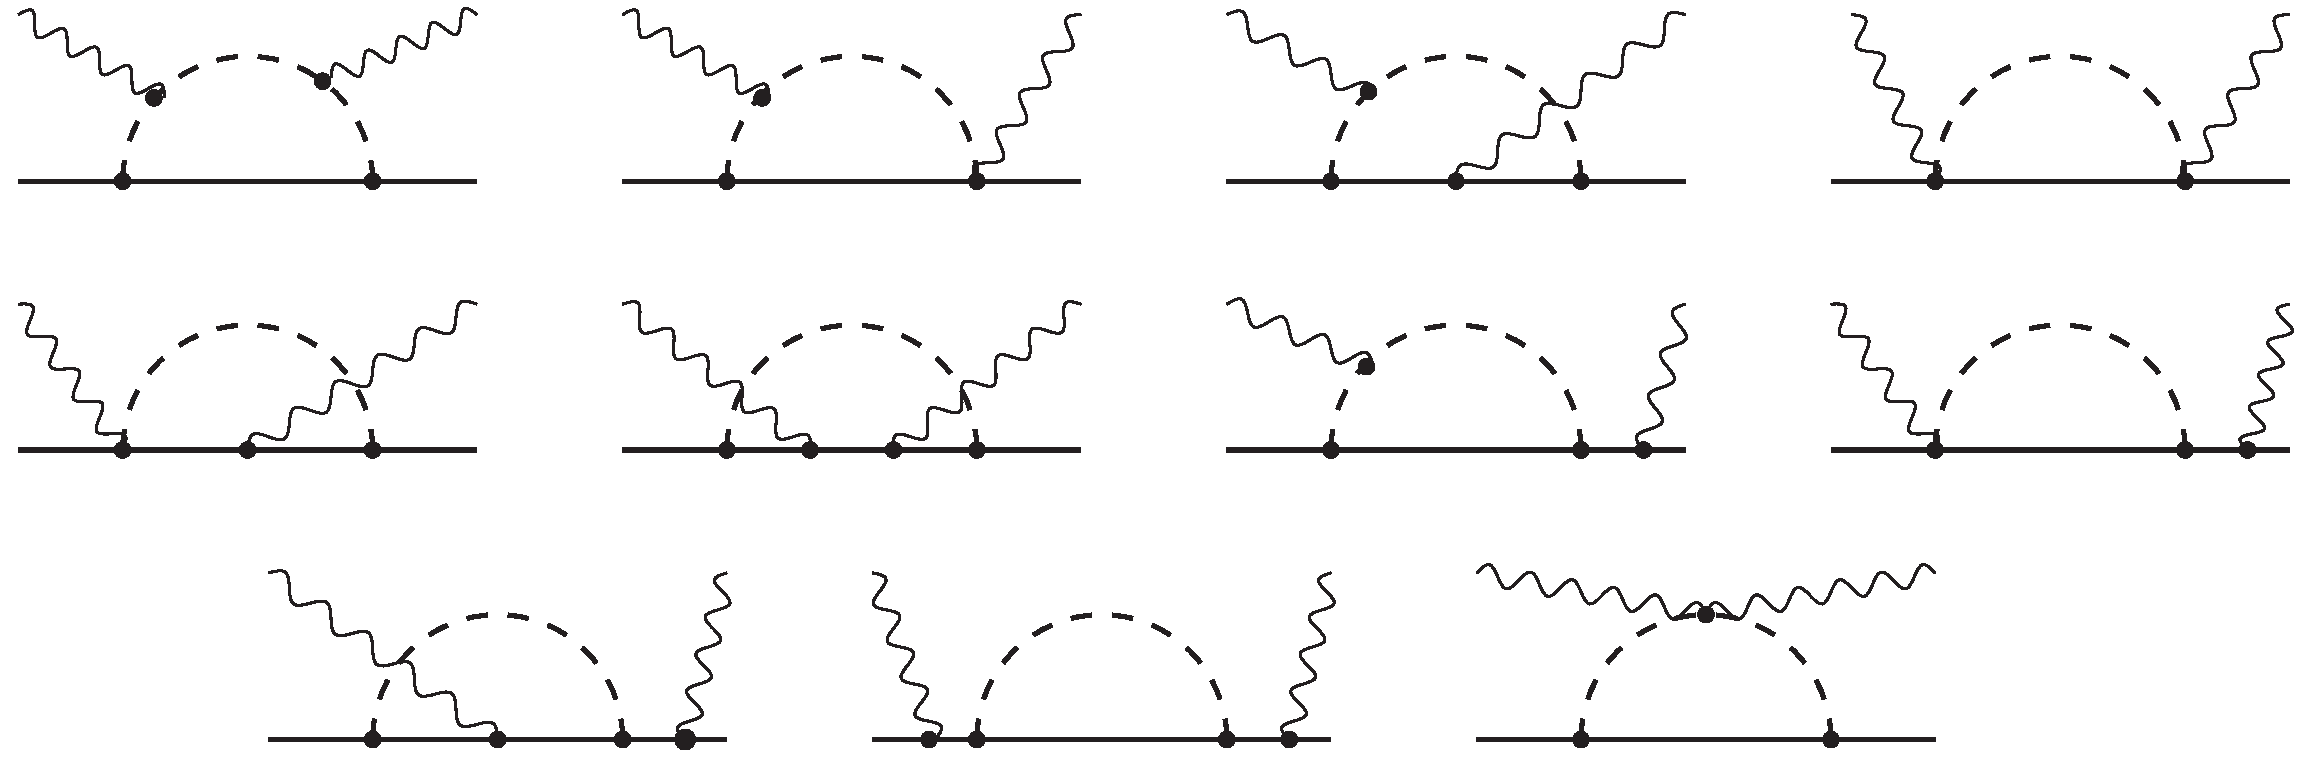
\includegraphics[width=0.95\columnwidth]{Diags1_pv.pdf} 
\caption{%(Color online)  
One-$\pi N$-loop graphs contributing to Compton scattering at $\mathcal{O}(p^3)$. Graphs obtained from these by
crossing and time-reversal are not shown, but are evaluated too.
}
\label{Fig:loops_pv}
\end{figure}

\begin{figure}[t]
\centering
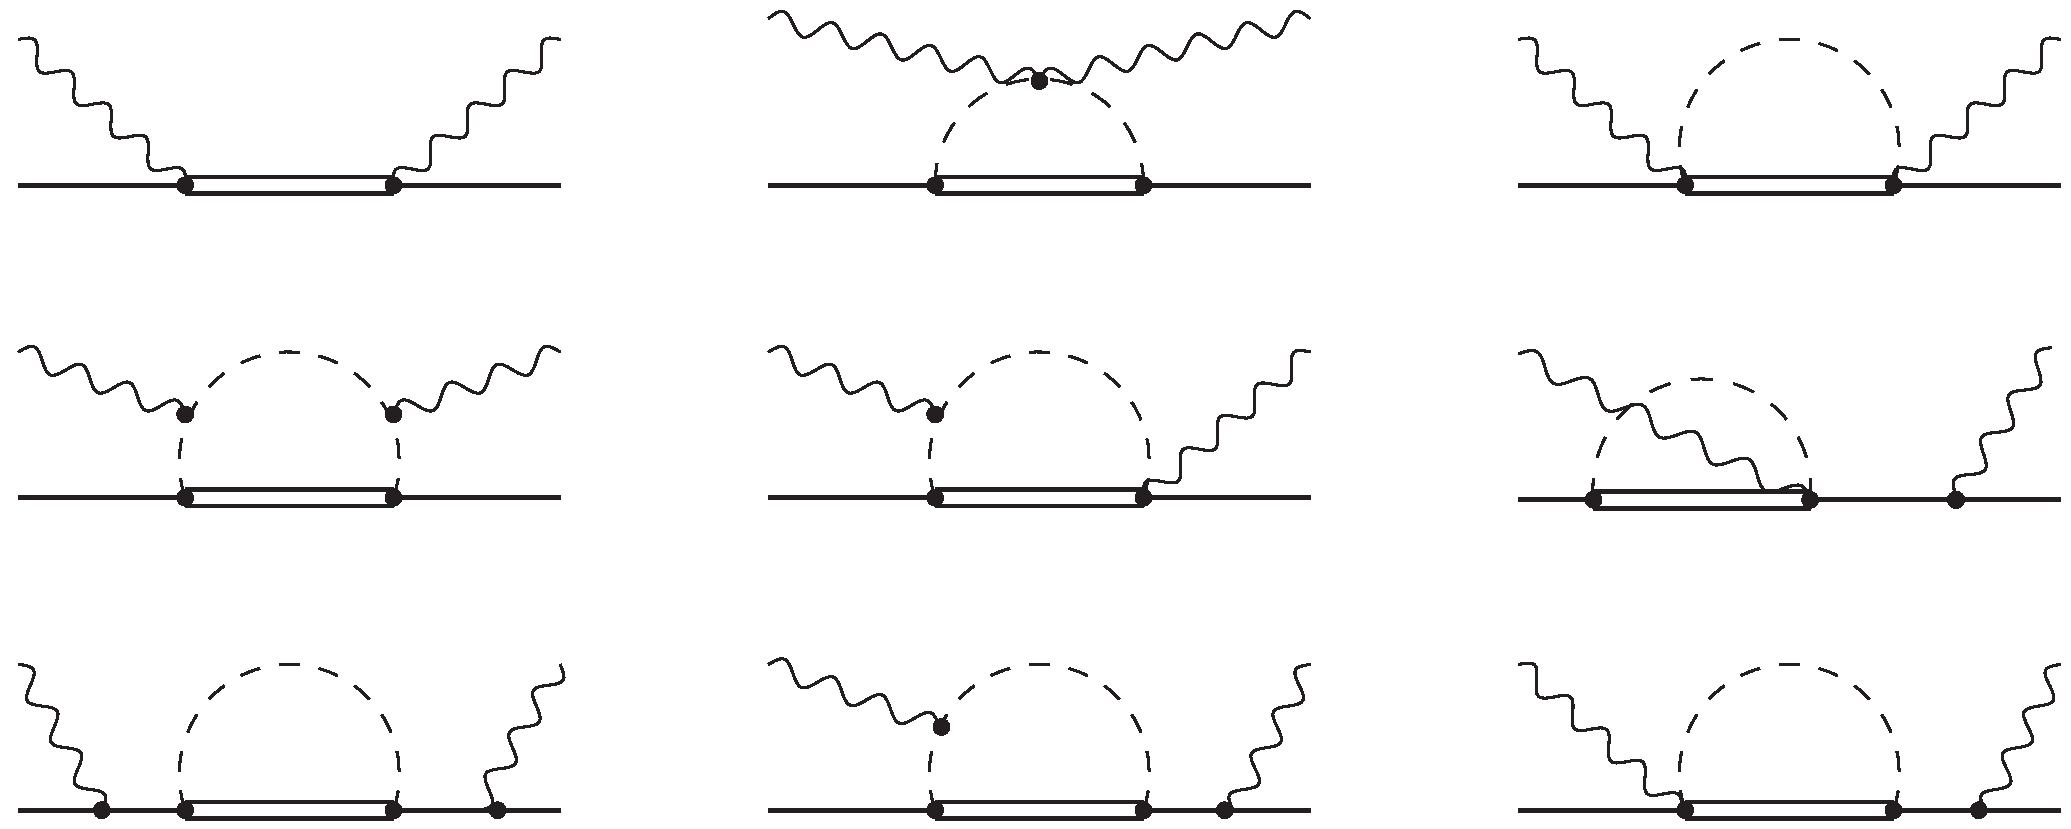
\includegraphics[width=0.95\columnwidth]{DeltaDiags4.pdf} 
\caption{%(Color online)  
Graphs contributing at  $\mathcal{O}(p^4/\mathit{\Delta})$. 
Double lines denote the propagator of the $\Delta$-isobar.
Graphs obtained from these by
crossing and time-reversal are evaluated too.}
\label{Fig:loopsD}
\end{figure}


\begin{figure*}
\begin{center}
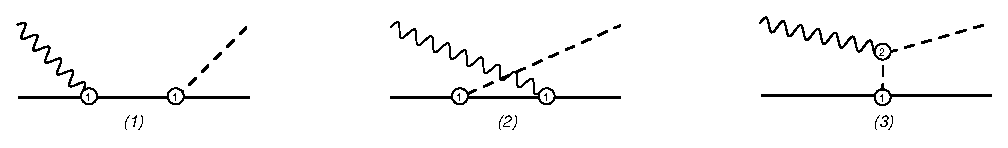
\epsfig{file=TreeLevelOp.eps,width=16cm,angle=0} 
\caption{This figures shows the diagrams that enter in our calculation of the pion electroproduction amplitude at leading order. The number in the vertices indicate the chiral order of each one.\label{Fig:DiagsOp}}
\end{center}
\end{figure*}

\begin{figure}
\begin{center}
\epsfig{file=sigmaLT.eps,width=8cm,angle=0} 
\caption{This figure illustrates the relation between the Compton and the photoabsorption part that are related via the optical theorem and contributes to $\delta_{LT}(\nu,Q^2)$. The double line arrows represent the polarization of the external particles, while the dot represents the scalar (longitudinal) polarization of the incoming photon. Inside the blob are represented the intermediate states: nucleons with spins $r'$ (which are averaged in the calculation of the cross section) and pions. \label{Fig:sigmaLT}}
\end{center}
\end{figure}

\begin{figure}[t]
\begin{center}
\hspace{-0.3cm}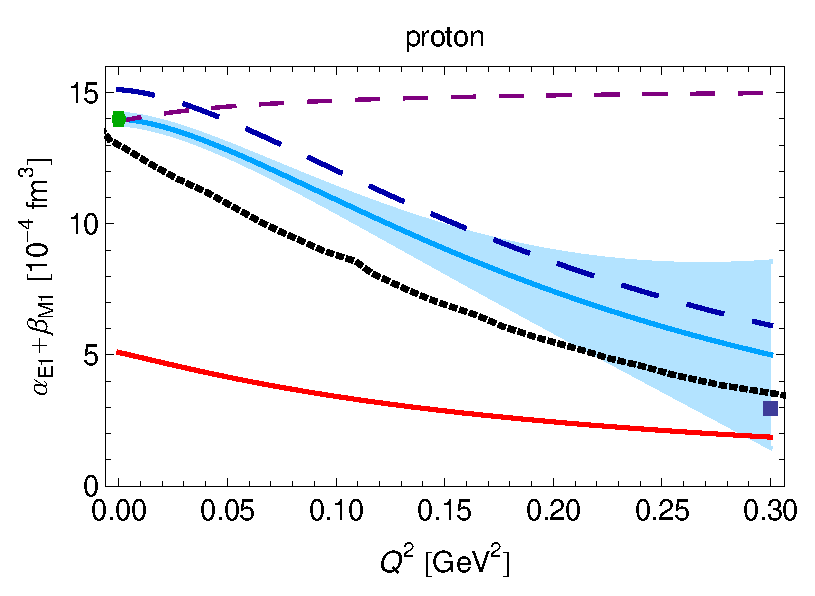
\epsfig{file=alpha+beta_p-Dip.eps,width=10cm,angle=0} \\
\hspace{-0.3cm}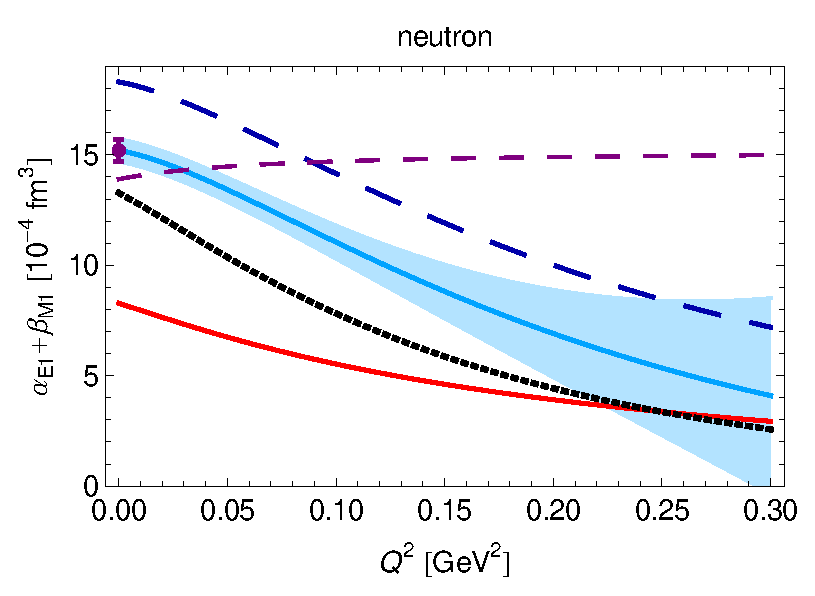
\epsfig{file=alpha+beta_n-Dip.eps,width=10cm,angle=0} 
\caption{Sum of electric and magnetic dipole polarizabilities, $\alpha_{E1}(Q^2)+\beta_{M1}(Q^2)$, for the proton ($p$) and neutron ($n$) as a function of $Q^2$.  
The results of this work is represented by the blue solid line and the blue band. The red line represents the pion cloud contribution in relativistic chiral EFT, while the blue dashed line is the leading order HB limit \cite{Nevado:2007dd}.
The black dotted line represents the MAID estimate \cite{Drechsel:2000ct,Drechsel:1998hk} given in Ref.~\cite{Drechsel:2002ar} for the proton, using $\pi+\eta+\pi\pi$ channels. The purple and red (under the purple one) dots at $Q^2=0$ correspond to the phenomenological extractions reported in \cite{OlmosdeLeon:2001zn} (p) and \cite{Babusci:1997ij} (p and n), respectively. 
At finite momentum transfer, in the region considered, we have available the $Q^2=0.3$~GeV$^2$ point (blue dot) obtained in Ref.~\cite{Liang:2004tk} through evaluation of the generalized Baldin sum rule. \label{Fig:alpha+betaplot}}
\end{center}
\end{figure}

\begin{figure}[t]
\begin{center}
\hspace{-0.3cm}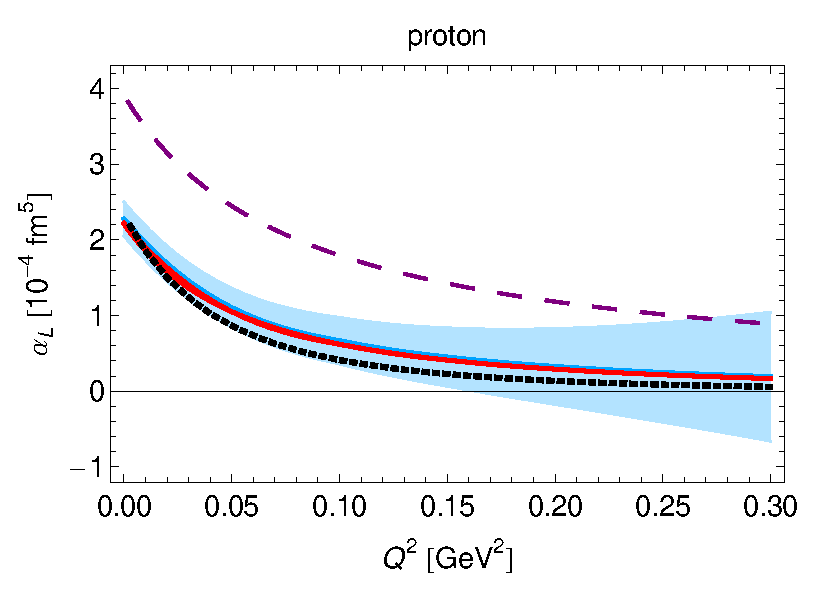
\epsfig{file=alphaL_p.eps,width=9cm,angle=0}\\ \hspace{-0.3cm}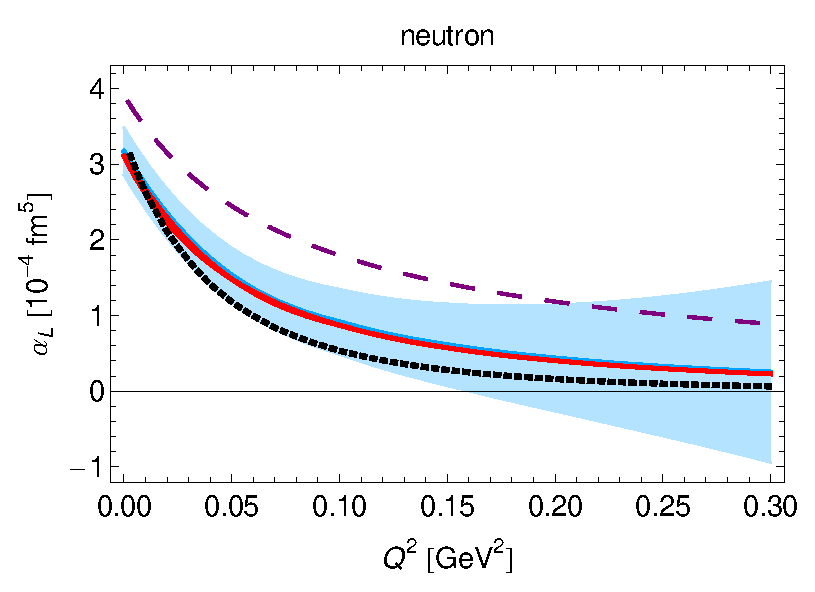
\epsfig{file=alphaL_n.eps,width=9cm,angle=0}
\caption{Longitudinal polarizabilities, $\alpha_L (Q^2)$, for the proton  (p) and neutron (n) as a function of $Q^2$. The legend is the same as in Fig.~\ref{Fig:alpha+betaplot} except for the black dotted line which correspond to the MAID estimate using only the $\pi$-channel, as in Ref.~\cite{Drechsel:2002ar}.  \label{Fig:alphaLplot}}
\end{center}
\end{figure}


\begin{figure}[t]
\begin{center}
\hspace{-0.3cm}\epsfig{file=gamma0_p-Dip.eps,width=9cm,angle=0}\\
 \hspace{-0.3cm}\epsfig{file=gamma0_n-Dip.eps,width=9cm,angle=0}
\caption{Forward spin polarizabilities, $\gamma_0(Q^2)$, for the proton (p) and neutron (n) as a function of $Q^2$. 
For the blue band and the red line the legend is the same as in Fig.~\ref{Fig:alpha+betaplot}. The $\mathcal{O}(p^3)+\mathcal{O}(p^4)$ HB results of Ref.~\cite{Kao:2002cp} is indicated by the blue short-dashed line, however for the proton the prediction lies outside the range of values displayed in the figure. 
The MAID curves, both in black dotted lines, are from Ref.~\cite{Drechsel:2002ar} in the case of the proton, and Ref.~\cite{Amarian:2004yf} in the case of the neutron. 
The experimental determinations for the proton are taken from Ref.~\cite{Prok:2008ev} (blue dots) and Ref.~\cite{Dutz:2003mm} (purple dot), while for the neutron the blue dots are from Ref.~\cite{Amarian:2004yf} and the greenish dots are from Ref.~\cite{Guler:2015} (statistical error in gray, systematic uncertainty in green). The grey band is the BChPT+$\Delta$ result of \cite{Bernard:2012hb}. \label{Fig:gamma0plot} }
\end{center}
\end{figure}



\begin{figure}[t]
\begin{center}
\hspace{-0.3cm}\epsfig{file=deltaLT_p-Dip.eps,width=9cm,angle=0} \\\hspace{-0.3cm}\epsfig{file=deltaLT_n-Dip.eps,width=9cm,angle=0} 
\caption{Longitudinal-transverse spin polarizabilities, $\delta_{LT}(Q^2)$, for the proton (p) and neutron (n) as a function of $Q^2$. 
For the blue band, the red line, and the black dotted line the legend is the same as in Fig.~\ref{Fig:alpha+betaplot}. 
The orange dot-dashed and blue short-dashed line are the $\mathcal{O}(p^3)$ and $\mathcal{O}(p^3)+\mathcal{O}(p^4)$ HB calculations of Ref.~\cite{Kao:2002cp}. The red band is the IR result of \cite{Bernard:2002pw} and the grey band is the covariant BChPT calculation including the $\Delta(1232)$ of Ref.~\cite{Bernard:2012hb}. 
The experimental points of $\delta^n_{LT}$ are from Ref.~\cite{Amarian:2004yf}.\label{Fig:deltaLTplot}}
\end{center}
\end{figure}

\begin{figure}[t]
\begin{center}
\hspace{-0.3cm}\epsfig{file=IAp-Dip.eps,width=9cm,angle=0} \\
\hspace{-0.3cm}\epsfig{file=IAn-Dip.eps,width=9cm,angle=0} 
\caption{Results for the generalized GDH integral for proton (p) and neutron (n) as a function of $Q^2$. For the blue band and the red line the legend is the same as in Fig.~\ref{Fig:alpha+betaplot}. The blue short-dashed line is the $\mathcal{O}(p^4)$ HB result of \cite{Kao:2002cp,Kao:2003jd} and the grey band is the BChPT+$\Delta$ result of \cite{Bernard:2012hb}. The black dotted line is the MAID model prediction. The experimental points for the neutron are from \cite{Amarian:2002ar}.\label{Fig:IAplot}}
\end{center}
\end{figure}

\begin{figure}[t]
\begin{center}
\hspace{-0.3cm}\epsfig{file=I1p-Dip.eps,width=9cm,angle=0} \\
\hspace{-0.3cm}\epsfig{file=I1n-Dip.eps,width=9cm,angle=0} 
\caption{Results for the integral $I_1$ for proton (p) and neutron (n) as a function of $Q^2$. The blue dashed line is the HB result of Ref.~\cite{Kao:2003jd}. The experimental points are from JLAB and the black dotted line is the MAID model prediction.\label{Fig:I1plot}}
\end{center}
\end{figure}

\begin{figure}
\begin{center}
\hspace{-0.3cm}\epsfig{file=Gamma1p-Dip.eps,width=9cm,angle=0} \\\hspace{-0.3cm}\epsfig{file=Gamma1n-Dip.eps,width=9cm,angle=0} 
\caption{First moment of the structure function $g_1$ for the proton (p) and neutron (n) as a function of $Q^2$. For the blue band and the red line the legend is the same as in Fig.~\ref{Fig:alpha+betaplot}. The blue dashed line is the HB result of Ref.~\cite{Kao:2003jd}, the grey band is the relativistic calculation of Ref.~\cite{Bernard:2012hb} and the dotted line is the MAID model prediction. The experimental points are from Ref.\cite{Prok:2008ev}.\label{Fig:Gamma1plot}}
\end{center}
\end{figure}

\begin{figure}
\begin{center}
\hspace{-0.3cm}\epsfig{file=Gamma1pn-Dip.eps,width=9cm,angle=0} 
\caption{Isovector combination of the first moment of $g_1$. The legend is the same as in Fig.~\ref{Fig:Gamma1plot}. The red thin band is the IR result of Ref.~\cite{Bernard:2002pw}. \label{Fig:Gamma1-isovector-plot}}
\end{center}
\end{figure}


\begin{figure}
\begin{center}
\hspace{-0.3cm}\epsfig{file=d2p-Dip.eps,width=9cm,angle=0} \\
\hspace{-0.3cm}\epsfig{file=d2n-Dip.eps,width=9cm,angle=0} 
\caption{Inelastic part of the moment $d_2$ for the proton (p) and neutron (n) as a function of $Q^2$. For the blue band and the red line the legend is the same as in Fig.~\ref{Fig:alpha+betaplot}. The black dotted line gives the MAID model prediction. The blue short-dashed line is the $\mathcal{O}(p^3)+\mathcal{O}(p^4)$ HB result of Ref.~\cite{Kao:2002cp,Kao:2003jd}.}
\end{center}
\end{figure}


\begin{figure}[H]
\begin{center}
\hspace{-0.3cm}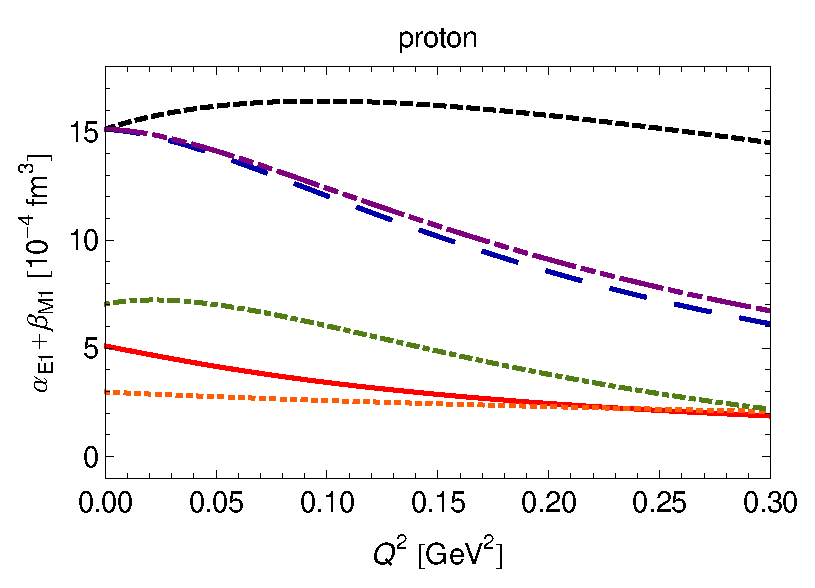
\epsfig{file=alpha+beta_p-orders-Dip.eps,width=9cm,angle=0}\\ \hspace{-0.3cm}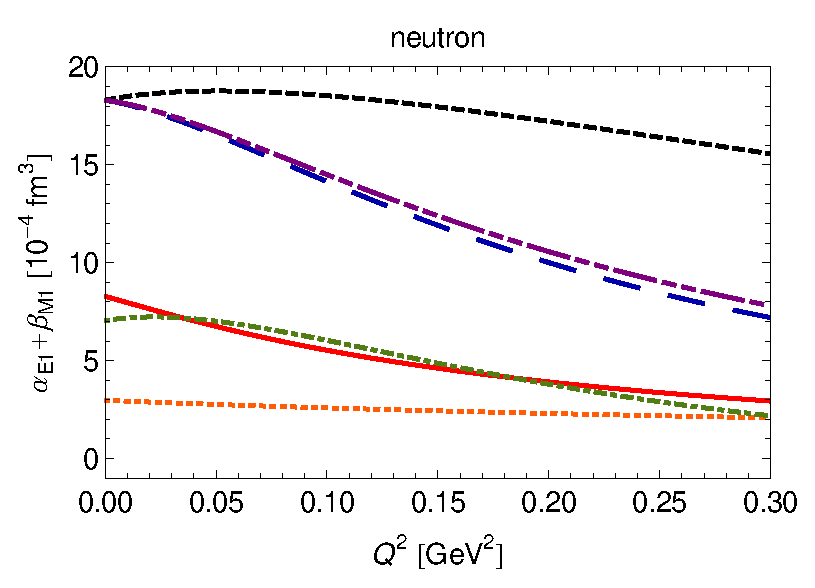
\epsfig{file=alpha+beta_n-orders-Dip.eps,width=9cm,angle=0} 
\caption{\small{Contribution of the different orders to the chiral prediction of $[\alpha_{E1}+\beta_{M1}](Q^2)$. Red dashed line: $\pi$-cloud contribution, green dot-dashed line: $\Delta$-pole contribution, orange dotted line: $\pi \Delta$ loops contribution, blue solid line: total, blue dashed line: total without $g_C$ contribution, purple dot-dot-dashed line: total result without dipole.}\label{Fig:alpha+beta-orders}}
\end{center}
\end{figure}

\begin{figure}[H]
\begin{center}
\hspace{-0.3cm}\epsfig{file=alphaL_p-orders.eps,width=9cm,angle=0}\\ \hspace{-0.3cm}\epsfig{file=alphaL_n-orders.eps,width=9cm,angle=0} 
\caption{Contribution of the different orders to the chiral prediction of $\alpha_{L}(Q^2)$. Red dashed line: $\pi$-cloud contribution, green dot-dashed line: $\Delta$-pole contribution, orange dotted line: $\pi \Delta$ loops contribution, blue solid line: total, blue dashed line: total without $g_C$ contribution, purple dot-dot-dashed line: total result without dipole. \label{Fig:alphaL-orders}}
\end{center}
\end{figure}

\begin{figure}[H]
\begin{center}
\hspace{-0.3cm}\epsfig{file=gamma0_p-orders-Dip.eps,width=9cm,angle=0}\\ \hspace{-0.3cm}\epsfig{file=gamma0_n-orders-Dip.eps,width=9cm,angle=0} 
\caption{Contribution of the different orders to the chiral prediction of $\gamma_0(Q^2)$. Red dashed line: $\pi$-cloud contribution, green dot-dashed line: $\Delta$-pole contribution, orange dotted line: $\pi \Delta$ loops contribution, blue solid line: total, blue dashed line: total without $g_C$ contribution, purple dot-dot-dashed line: total result without dipole. \label{Fig:gamma0-orders}}
\end{center}
\end{figure}
 

\begin{figure}[H]
\begin{center}
\hspace{-0.3cm}\epsfig{file=deltaLT_p-orders-Dip.eps,width=9cm,angle=0}\\ \hspace{-0.3cm}\epsfig{file=deltaLT_n-orders-Dip.eps,width=9cm,angle=0} 
\caption{Contribution of the different orders to the chiral prediction of $\delta_{LT}(Q^2)$. ed dashed line: $\pi$-cloud contribution, green dot-dashed line: $\Delta$-pole contribution, orange dotted line: $\pi \Delta$ loops contribution, blue solid line: total, blue dashed line: total without $g_C$ contribution, purple dot-dot-dashed line: total result without dipole.  \label{Fig:deltaLT-orders}}
\end{center}
\end{figure}

\begin{figure}[t]
\begin{center}
\hspace{-0.3cm}\epsfig{file=IAp-Dip-orders.eps,width=9cm,angle=0}\\ \hspace{-0.3cm}\epsfig{file=IAn-Dip-orders.eps,width=9cm,angle=0} 
\caption{Contribution of the different orders to the chiral prediction of $I_A(Q^2)$. Red dashed line: $\pi$-cloud contribution, green dot-dashed line: $\Delta$-pole contribution, orange dotted line: $\pi \Delta$ loops contribution, blue solid line: total, blue dashed line: total without $g_C$ contribution, purple dot-dot-dashed line: total result without dipole. \label{Fig:IA-orders-plot}}
\end{center}
\end{figure}

\begin{figure}[t]
\begin{center}
\hspace{-0.3cm}epsfig{file=I1p-Dip-orders.eps,width=9cm,angle=0}\\ \hspace{-0.3cm}\epsfig{file=I1n-Dip-orders.eps,width=9cm,angle=0} 
\caption{Contribution of the different orders to the chiral prediction of $\Delta I_1(Q^2)$. Red dashed line: $\pi$-cloud contribution, green dot-dashed line: $\Delta$-pole contribution, orange dotted line: $\pi \Delta$ loops contribution, blue solid line: total, blue dashed line: total without $g_C$ contribution, purple dot-dot-dashed line: total result without dipole. \label{Fig:I1-orders-plot}}
\end{center}
\end{figure}

%\begin{figure}
%\begin{center}
%\epsfig{file=I1p-NoDip.eps,width=8cm,angle=0} \epsfig{file=I1n-NoDip.eps,width=8cm,angle=0} 
%\caption{Comparison of the full result without dipole (red solid line) with the rest of the available ChPT calculations for $I_{1}$. The blue solid line and its band is our total result with dipole, and the blue dashed line is the HB result (Ref.~\cite{Kao:2002cp}) and the grey band is the BChPT+$\Delta$ result of \cite{Bernard:2012hb}. The data are the same as in Fig~\ref{Fig:I1plot}.\label{Fig:I1-NoDip}}
%\end{center}
%\end{figure}


%\begin{figure}
%\begin{center}
%\epsfig{file=Gamma1p-NoDip.eps,width=8cm,angle=0} \epsfig{file=Gamma1n-NoDip.eps,width=8cm,angle=0} 
%\caption{Comparison of the full result without dipole (red solid line) with the rest of the available ChPT calculations for $\Gamma_{1}$. The blue solid line and its band is our total result with dipole, and the blue dashed line is the HB result (Ref.~\cite{Kao:2002cp}) and the grey band is the BChPT+$\Delta$ result of \cite{Bernard:2012hb}. The data are the same as in Fig~\ref{Fig:Gamma1plot}.\label{Fig:Gamma1-NoDip}}
%\end{center}
%\end{figure}


%\begin{figure}
%\begin{center}
%\epsfig{file=alpha+beta_p-NoDip.eps,width=8cm,angle=0} \epsfig{file=alpha+beta_n-NoDip.eps,width=8cm,angle=0} 
%\caption{Comparison of the full result without dipole (red solid line) with the rest of the available ChPT calculations for $\alpha+\beta$. The blue solid line and its band is our total result with dipole and the blue dashed line is the leading order result of \cite{Nevado:2007dd}. The data are the same as in Fig~\ref{Fig:alpha+betaplot}.\label{Fig:alpha+beta-NoDip}}
%\end{center}
%\end{figure}

%\begin{figure}
%\begin{center}
%\epsfig{file=IAp-NoDip.eps,width=8cm,angle=0} \epsfig{file=IAn-NoDip.eps,width=8cm,angle=0} 
%\caption{Comparison of the full result without dipole (red solid line) with the rest of the available ChPT calculations for $I_{A}$. The blue solid line and its band is our total result with dipole, and the blue dashed line is the HB result (Ref.~\cite{Kao:2002cp}) and the grey band is the BChPT+$\Delta$ result of \cite{Bernard:2012hb}. The data are the same as in Fig~\ref{Fig:IAplot}.\label{Fig:IA-NoDip}}
%\end{center}
%\end{figure}

%\begin{figure}
%\begin{center}
%\epsfig{file=d2p-NoDip.eps,width=8cm,angle=0} \epsfig{file=d2n-NoDip.eps,width=8cm,angle=0} 
%\caption{Comparison of the full result without dipole (red solid line) with the rest of the available ChPT calculations for $\bar{d}_{2}$. The blue solid line and its band is our total result with dipole, and the blue dashed line is the HB result (Ref.~\cite{Kao:2002cp}) and the grey band is the BChPT+$\Delta$ result of \cite{Bernard:2012hb}. The data are the same as in Fig~\ref{Fig:d2plot}.\label{Fig:d2-NoDip}}
%\end{center}
%\end{figure} 

%\begin{figure}
%\begin{center}
%\epsfig{file=deltaLT_p-NoDip.eps,width=8cm,angle=0} \epsfig{file=deltaLT_n-NoDip.eps,width=8cm,angle=0} 
%\caption{Comparison of the full result without dipole (red solid line) with the rest of the available ChPT calculations for $\delta_{LT}$. The blue solid line and its band is our total result with dipole, and the blue dashed line is the HB result (Ref.~\cite{Kao:2002cp}) and the grey band is the BChPT+$\Delta$ result of \cite{Bernard:2012hb}. The data are the same as in Fig~\ref{Fig:deltaLTplot}.\label{Fig:deltaLT-NoDip}}
%\end{center}
%\end{figure}

%\begin{figure}
%\begin{center}
%\epsfig{file=gamma0_p-NoDip.eps,width=8cm,angle=0} \epsfig{file=gamma0_n-NoDip.eps,width=8cm,angle=0} 
%\caption{Comparison of the full result without dipole (red solid line) with the rest of the available ChPT calculations for $\gamma_0$. The blue solid line and its band is our total result with dipole, the blue dashed line is the HB result (Ref.~\cite{Kao:2002cp}) and the grey band is the BChPT+$\Delta$ result of \cite{Bernard:2012hb}. The data are the same as in Fig~\ref{Fig:gamma0plot}.\label{Fig:gamma0-NoDip}}
%\end{center}
%\end{figure}


\end{document}